\documentclass[12pt,UTF8,aspectratio=169]{beamer} 
\RequirePackage{mybeamer}
%%% sudo vim /usr/local/texlive/2021/texmf-dist/tex/xelatex/mybeamer
%%%% sudo texhash

%\usepackage{hyperref}
%\hypersetup{
%    colorlinks=true,
%    linkcolor=blue,
%    filecolor=blue,      
%    urlcolor=blue,
%    citecolor=cyan,
%    pdfpagemode=FullScreen,
%}

%-------------------正文-------------------------%
%                                               %
%                                               %
\begin{document}                                %
%                                               %
%                                               %
%-----------------------------------------------%

%题目,作者,学校,日期                
\author{\myfont 李小飞}
\title{\textbf{\Huge 工~程~数~学}}
\subtitle{Engineering Mathematics}
\institute[电子科技大学]{{\large 光电科学与工程学院}}
\date{\today}

	%%%%%%%%%%%%%%%%%%%%%%%%%%%%%%%%%
    %\frame[plain]{\titlepage}
    %%%%%%%%%%%%%%%%%%%%%%%%%%%%%%%%%
    \begin{frame}{目录}
        \setbeamertemplate{section in toc}[sections numbered]
        \tableofcontents[hideallsubsections]
    \end{frame}%%%


%\maketitle

%------------------- 章节-------------------------%
%\section{课程简介}

\begin{frame}
  \begin{algorithm}[H]
    \SetAlgoLined
    \KwData{this text}
    \KwResult{how to write algorithm with \LaTeX2e }
    initialization\;
    \While{not at end of this document}{
        read current\;
        \eIf{understand}{
            go to next section\;
            current section becomes this one\;
            }{
            go back to the beginning of current section\;
        }
    }
\caption{How to write algorithms}
\end{algorithm}

\end{frame}

\begin{frame}
  \begin{proof}
    This is a proof
  \end{proof}

\end{frame}

\begin{frame}
  \tcbset{colback=white,arc=0mm,width=(\linewidth-4pt)/4,
  equal height group=AT,before=,after=\hfill,fonttitle=\bfseries}
  
  \noindent
  \foreach \n in {xxx,ggg,AAA,\"Agypten}
  {\begin{tcolorbox}[title=\n,colframe=red!75!black]
    Some content.\end{tcolorbox}}
  
  \noindent
  \foreach \n in {xxx,ggg,AAA,\"Agypten}
  {\begin{tcolorbox}[adjusted title=\n,colframe=blue!75!black]
  Some content.\end{tcolorbox}}
  
  \begin{tcbitemize}[raster columns=3,raster equal height,
            colframe=red!75!black,colback=red!5!white,fonttitle=\bfseries]
  \tcbitem[squeezed title={Short title}]
  First box
  \tcbitem[squeezed title={This is a very very long title}]
  Second box
  \tcbitem[squeezed title={This title is clearly to long for this application}] Third box
  \end{tcbitemize}
  
  \begin{tcbitemize}[raster columns=3,raster equal height,
            colframe=blue!75!black,colback=red!5!white,fonttitle=\bfseries]
  \tcbitem[squeezed title*={Short title}]
  First box
  \tcbitem[squeezed title*={This is a very very long title}]
  Second box
  \tcbitem[squeezed title*={This title is clearly to long for this application}] Third box
  \end{tcbitemize}
\end{frame}


\begin{frame}
  \begin{tcolorbox1}{title}
    This is tcolorbox1
  \end{tcolorbox1}
  \begin{tcolorbox1}[2]{title}
    This is tcolorbox1
  \end{tcolorbox1}
  \begin{tcolorbox2}{title}
    This is tcolorbox2
  \end{tcolorbox2}
  \begin{tcolorbox}{title}
    This is tcolorbox
  \end{tcolorbox}
\end{frame}
                   %
%                                               %
%%%%%%%%%%%%%%%%%%%%%%%%%%%%%%%%%%%%%%%%%%%%%%%%%%
	\begin{frame}
		\frametitle{}
	    \begin{center}
		{ {\Huge 第一章~~绪~论 (4课时)}}
	    \end{center}    
	\end{frame}

%%%%%%%%%%%%%%%%%%%%%%%%%%%%%%%%%%%%%%%%%%%%%%
\section{课程介绍}

\begin{frame}
\frametitle{课程介绍}
	\begin{center}
		\begin{figure}
		\begin{minipage}[t]{0.4\textwidth}
			\includegraphics[width=4.5cm]{figs/fig1-2.png}	
			%\caption{}
		\end{minipage}
		\begin{minipage}[t]{0.4\textwidth}
			\includegraphics[width=3.0cm]{figs/fig1-2-2.png}	
			%\caption{}
		\end{minipage}
		\end{figure}
	17世纪微积分出现,物理学家写方程,数学物理学家解方程,试图通过方程理解大千世界。
  	\end{center}
\end{frame}

\begin{frame}
	\frametitle{数理方程在数学中的位置}
	\begin{center}
		\begin{figure}
			\includegraphics[width=7cm]{figs/fig1-1.png}	
			%\caption{}
		\end{figure}
		{ 数学:逻辑,计算,分析,统计,结构}
	\end{center}
\end{frame}
%3%

\subsection{主要内容}

\begin{frame}
	\frametitle{教学内容}
	\begin{enumerate}
			\item 第一章 ~绪论(4学时):常微分方程及其解法、傅里叶变换
			 \vspace{0.2cm}
			 \item 第二章~ 偏微分方程(6学时):波动方程、热传导方程、拉普拉斯方程。
			 \vspace{0.2cm}
			 \item 第三章 ~薛定谔方程(6学时):无限深势阱、量子谐振子、Hermite多项式
            \vspace{0.2cm}
            \item 第四章 ~氢原子薛定谔方程(10学时):勒让德方程、拉盖尔(Laguerre)方程
            \vspace{0.2cm}
            \item 第五章~ 特殊函数及其应用(6学时):贝塞尔(Bessel)方程、Bessel函数
     \end{enumerate}	
\end{frame}

\begin{frame}
	\frametitle{}
	\begin{center}
		\begin{figure}
			\includegraphics[width=4.5cm]{figs/fig1-3-1.png}	
		\end{figure}
	\end{center}
	{数理方程大牛-拉普拉斯(法):拉普拉斯方程,天体力学,比如描述引力势能,时间1770年代(乾隆年间)}
\end{frame}

\begin{frame}
	\frametitle{}
	\begin{center}
		\begin{figure}
			\includegraphics[width=4.5cm]{figs/fig1-3-4.png}	
		\end{figure}
	\end{center}
		{泊松(法):Laplace方程原来是Poisson方程的特例,描述场(电场,引力场等等)}
\end{frame}

\begin{frame}
	\frametitle{}
	\begin{center}
		\begin{figure}
			\includegraphics[width=4.5cm]{figs/fig1-3-5.png}	
		\end{figure}
	\end{center}
		{勒让德(法):球坐标系下的拉普拉斯方程,可转化为勒让德方程。球谐函数,薛定谔方程解氢原子}
\end{frame}

\begin{frame}
	\frametitle{}
	\begin{center}
		\begin{figure}
			\includegraphics[width=4.5cm]{figs/fig1-3-2.png}	
		\end{figure}
	\end{center}
		{格林(英):Laplace方程无源场,泊松方程有源场,解是格林函数的叠加}
\end{frame}

\begin{frame}
	\frametitle{}
	\begin{center}
		\begin{figure}
			\includegraphics[width=4.5cm]{figs/fig1-3-3.png}	
		\end{figure}
	\end{center}
	{傅里叶(法国):分离变量法解波动方程,积分变换法解热传导方程,傅里叶级数和傅里叶变换}
\end{frame}

\begin{frame}
	\frametitle{}
	\begin{center}
		\begin{figure}
			\includegraphics[width=4.5cm]{figs/fig1-3-7.png}	
		\end{figure}
	\end{center}
	{达朗贝尔(法国):波动方程的通解,麦克斯韦方程、电磁波}
\end{frame}

\begin{frame}
	\frametitle{}
	\begin{center}
		\begin{figure}
			\includegraphics[width=4.5cm]{figs/fig1-3-6.png}	
		\end{figure}
	\end{center}
	{贝塞尔(德国):柱坐标系下的拉普拉斯方程,可转化为贝塞尔方程,解是一系列贝塞尔函数}
\end{frame}

\begin{frame}
	\frametitle{}
	\begin{center}
		\begin{figure}
			\includegraphics[width=4.5cm]{figs/fig1-3-8.png}	
		\end{figure}
	\end{center}
	{爱因斯坦(德国):扩散方程和热传导方程同类,原创扩散方程新解法(布朗运动),爱因斯坦方程}
\end{frame}

\begin{frame}
	\frametitle{}
	\begin{center}
		\begin{figure}
			\includegraphics[width=4.5cm]{figs/fig1-3-9.png}	
		\end{figure}
	\end{center}
	{薛定谔:1926年,薛定谔方程,解氢原子、氦原子,氢分子、... }
\end{frame}
%6
\begin{frame}
	\frametitle{教材与教参 :}
	\begin{enumerate}
		\item 教材:《工程数学讲义》 李明奇,钟尔杰,国防工业出版社, 待出版\\	\vspace{0.3cm}
     	参考资料:\\
		\item 《数学物理方程》 李明奇、田太心,电子科技大学出版社,2014
		\vspace{0.3cm}
		\item 《数学物理方法》 姚瑞正,梁家宝 ,武汉大学出版社,1992
		\vspace{0.3cm}
		\item 《数学物理方程与特殊函数》南京工学院数学教研组,人民教育出版社,1983
		\vspace{0.3cm}
		\item 《数学物理方程》孙振绮,机械工业出版社,2004
	\end{enumerate}	
\end{frame}

\subsection{成绩构成}
\begin{frame}
	\frametitle{成绩构成:}
		\begin{enumerate}
		\item 平时作业:10\%,
		\vspace{0.8cm}
		\item 课堂讨论:10\%,
		\vspace{0.8cm}
		\item 测验:~~ 10\%,
		\vspace{0.8cm}
		\item 期末考试:70\% .
		\end{enumerate}	
\end{frame}

%%%%%%%%%%%%%%%%%%%%%%%%%%%%%%%%%%%%%%%%%%%%%
\section{常微分方程}
\subsection{衰减与增长模型}
\begin{frame}
	\frametitle{微分方程及基本解法:}
    \begin{enumerate}
    \item 微分方程:含未知函数及其导数的方程 \\
    	$f\left(x,t, u, u_t,u_{tt}, \ldots u_{t \ldots t}, u_{x}, u_{xx}, \ldots, u_{x \ldots x} \right)=0$ \\
    	\vspace{0.5cm}
 		物理量(u)一般是时间和空间的函数。解微分方程就是要求出u(x,t)。根据阶分类;一阶微分方程、二阶微分方程、高阶常微分方程。
	 	根据未知函数自变量数目分类:常微分方程(单变量)、偏微分方程(多变量) 
    	\vspace{0.5cm}
    \item 基本解法:行波法、分离变量法、积分变换法、格林函数法、保角变换法、复变函数法、变分法、级数展开法         
    \end{enumerate}
\end{frame}

\begin{frame}
	\frametitle{一阶常微分方程}
	{\large 形态:$g(y)dy=f(x)dx$ }\\ \vspace{0.6cm}
	\textbf{解法:}若 $g(y)$ , $f(x)$ 连续 ,有\\	\vspace{0.3cm}
   	{\large 	$\int$ g(y) d y=$\int$ f(x) d x }\\	\vspace{0.3cm}
	若$g(y)$, $f(x)$  有原函数,通解为\\	\vspace{0.3cm}
	{\large $G(y)=F(x)+C$}\\	\vspace{0.3cm}
	定解条件确定C,得解!
\end{frame}

\begin{frame}
\frametitle{衰减与增长模型}
	\begin{block}{指数增长和衰减}
	\begin{itemize}
		\item 衰减与增长模型,自然界和人类社会客观存在。
		\item 分别采用指数衰减和指数增长描述,
		\item 速度大于零为增长模型,小于零为衰减模型。
	\end{itemize}
	\end{block}
\end{frame}

\begin{frame}
	\begin{exampleblock} {例1、	求解放射性衰减模型}
	\begin{equation*}
	\frac{du}{dt}	= - ru, ~~~~ u(t_0) = u_0
	\end{equation*}
	\end{exampleblock} 	
	\alert{解:} 方程可分离变量:
	\begin{align*}
		\frac{du}{u} &= - rdt\\
		\ln u &=-rt+C\\
		u(t)&=C’exp(-rt)	
	\end{align*}
	令$t=0$, 有$C‘=u_0$,得定解:
	\begin{equation*}
		u(t)=u_0 exp(-rt)
	\end{equation*}
\end{frame}


\begin{frame}
\begin{block} {Remark}
	显然,当$r>0$时, 有$t \to \infty$, $u(t) \to 0$,  衰减模型中的一个重要问题是求半衰期 T\\
	\alert{解:} 
	\begin{align*}
	\frac{1}{2}u_0 &=u(T) =u_0 exp(-rT)\\
	T &=\frac{1}{r} \ln 2  \approx \frac{1}{r} \times 0.6931	
	\end{align*}
	\end{block}
\end{frame}

\begin{frame}
	\begin{exampleblock} {例2、	求人口增长的逻辑斯蒂模型}
	\begin{equation*}
		\frac{d u}{d t}=r u (1-u/K)
	\end{equation*}
	\end{exampleblock} 	
	\alert{解:} 方程可分离变量:
	\begin{align*}
		&\frac{1}{u(1-u / K)}du =r d t \\
		&\frac{u / K+(1-u / K)}{u(1-u / K)} d u =r d t	\\
		&(\frac{1}{K-u}+\frac{1}{u} ) d u =r d t \\
		&-\ln (K-u)+\ln u =r t+C \\
	\end{align*}	
\end{frame}

\begin{frame}
	\begin{align*}
		&\ln \frac{u}{K-u}  =r t+C\\
		&\frac{u}{K-u} =\exp (r t+C)\\
		&u(t)  =\frac{K}{1+\exp (-r t-C)}	\\
	\end{align*}	
	\begin{block} {问题:}
	建立并求解:冠状病毒感染人数增长模型
	\end{block}    
\end{frame}

\begin{frame}
	\frametitle{一阶齐次方程 }
	\begin{exampleblock} {例3、	求解如下一阶微分方程}
	\begin{equation*}
		\frac{d y}{d x}=f\left(\frac{y}{x}\right) 
	\end{equation*}
	\end{exampleblock} 	
	\alert{解:} 令:$\dfrac{y}{x}=u$, 有:$y=xu$ \\ 
	求微分: $ \dfrac{d y}{d x}=u+x \dfrac{d u}{d x}$,	代回方程:\\	
	 $ u+x \dfrac{d u}{d x}=f(u) , \to \dfrac{d u}{d x}=\dfrac{f(u)-u}{x}$ ,\\ \vspace{0.2cm}
	可分离变量:
	\begin{align*}
		\int \dfrac{d u}{f(u)-u}=\int \dfrac{d x}{x} 
	\end{align*}	
\end{frame}

\begin{frame}
\begin{exampleblock} {例4、	求解一阶微分方程}
	\begin{equation*}
	\left(x-y \cos \frac{y}{x}\right) d x+x \cos \frac{y}{x} d y=0
	\end{equation*}
\end{exampleblock} 	
\alert{解:} 变量代换后可分离变量,令$\frac{y}{x}=u$, 有:$y=xu$ , \\ 
		求微分:	$d y=x d u+u d x$ ~~~~, 
		代回原方程, 得:
		\begin{equation*}
			(x-u x \cos u) d x+x \cos u(u d x+x d u)=0
		\end{equation*}	
		整理, 得可分离变量方程:
		\begin{equation*}
			\cos udu=-\frac{dx}{x}
		\end{equation*}	
		两边积分
		\begin{equation*}
			\sin u=-\ln x+C, \to  \sin \frac{y}{x}=-\ln x+C
		\end{equation*}	
\end{frame}


\begin{frame}
	\frametitle{一阶非齐次方程}
	\begin{exampleblock} {例5、	求一阶变系数非齐次方程}
	\begin{equation*}
		y^{\prime}+P(x) y=Q(x)
	\end{equation*}
	\end{exampleblock} 
	\alert{解:}  常数变易法可求解,一阶齐次线性方程 :\\
		$ y^{\prime}+P(x) y=0$  \\ 
	有通解:	{\large 	$y=Ce^{-\int P(x)dx}$}\\	\vspace{0.3cm}
		令: $C=C(x)$ ,	{\large 	$ \to y=C(x)e^{-\int P(x)dx}$} \\ 
		代回原方程:
		\begin{equation*}
			C^{\prime}(x)=\frac {Q(x)} {e^{-\int P(x)dx}}
		\end{equation*}	
\end{frame}

\begin{frame}	
		两边积分
		\begin{equation*}
			C(x)=\int Q(x)e^{\int P(x)dx} dx+c 
		\end{equation*}	
		代回通解,得解:
		\begin{equation*}
			y=Ce^{-\int P(x)dx}+e^{-\int P(x)dx}\int Q(x)e^{\int P(x)dx} dx
		\end{equation*}	
\end{frame}

\begin{frame}
	\begin{exampleblock} {例6、	求一阶常系数非齐次线性方程}
	\begin{equation*}
		y^{\prime}+Py=Q(x)
	\end{equation*}
	\end{exampleblock} 
	\alert{解:} 例5方程的解中,取P(x)=P, 得解:
	\begin{equation*}
		y=Ce^{-\int Pdx}+e^{-\int Pdx}\int Q(x)e^{\int Pdx} dx
	\end{equation*}	
\end{frame}

\begin{frame}
	\begin{exampleblock} {例7、	积分因子法求一阶全微分方程}
	\begin{equation*}
	P(x,y)dx+Q(x,y)dy=0
	\end{equation*}
	\end{exampleblock} 
	\alert{解、}  存在u(x,y),使 $ du=P(x,y)dx+Q(x,y)dy $ 成立的\\
    充要条件为:{$\dfrac{\partial P }{\partial x}=\dfrac{\partial Q }{\partial y}$ }\\	
	得通解:	{  $\displaystyle { u(x,y)=\int P(x,y)dx+\int Q(x,y)dy} $}\\ 
	若不存在,可找个积分因子 $f(x,y) $ 乘以原方程 \\  \vspace{0.2cm}
	\textbf{比如:}{\large    $ydx-xdy=0$ } 不是全微分方程,\\ 
	但 $\dfrac{ydx-xdy}{y^2}=d(\dfrac{x}{y})$ 是全微分方程, 即找到积分因子{  $ \dfrac{1}{y^2}$ } !
\end{frame}

\subsection{振动模型}

\begin{frame}
	\frametitle{振动模型}
	\begin{exampleblock} {例 8、建立简谐振动微分方程并求解}	
	\begin{center}
		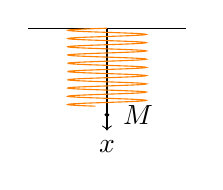
\begin{tikzpicture} [scale=0.5]
	\draw  (-2,0) -- (2,0) node[below] {};
	\draw [->] (0,0) -- (0,-2.6) node[below] {$x$};	
	\draw [orange, domain=0:-1.98, samples=200] plot({sin(\x r *30},\x);
	\draw [fill, black, circle] (0,-2.2) circle(0.3ex) node[right] {$M$};
    \end{tikzpicture} 
	\end{center}
	\end{exampleblock}
	\alert{解、} 根据牛顿第二定律,建立方程:\\
	\begin{equation*}
		F= -k x, ~~	F=Ma= M\frac{d ^2 x}{d t^2} 
	\end{equation*}
	\begin{equation*}
		\frac{d ^2 x}{d t^2} +\frac{k}{M} x =0, 
	\end{equation*}	
\end{frame}

\begin{frame}	
	得方程:
	$\displaystyle \begin{cases}
	\dfrac{d ^2 x}{d t^2} +\omega ^2 x = 0	\\
	x(t)\left |_{t=0}  =x_0  \right. , \\
	 \dfrac{dx}{dt} \left |_{t=0}  =0 \right.      	
	\end{cases}$\\
	\begin{block}{Remark}
	是常系数二阶齐次线性微分方程,通过辅助方程求解。 
	\end{block}
\end{frame}

\begin{frame}
	求解辅助方程: $u^2+\omega ^2=0$ \\
	\begin{equation*}
		u_{1, 2} =\pm i\omega     
	\end{equation*}
	方程的基本解: 
	\begin{equation*}
		x_{1} =\cos \omega t  , ~~~~	x_{2} =\sin \omega t     
	\end{equation*}
	方程通解: $x(t)=C_1 \cos \omega t +C_2 \sin \omega t $ \\  	\vspace{0.6cm}
	由初始条件得特解: $x(t)=x_0 \cos \omega t $ \\
\end{frame}

\begin{frame}
	\begin{exampleblock} {例9、	求解如下小阻尼振动微分方程:}
	\begin{equation*}
		\frac{d^2 u}{d t^2} +2\varepsilon \frac{d u}{dt} +\omega ^2 u = 0 ,  ~~~ (\varepsilon < \omega)   
	\end{equation*}
	\end{exampleblock} 
	\alert{解、} 令 $\displaystyle  u(t)= exp(-\varepsilon t) v(t) $,求微分,得:\\	
	\begin{align*}
		\frac{d u}{d t } & =exp(-\varepsilon t) [-\varepsilon v +\frac{d v}{dt}]\\
		\frac{d^2 u}{d t^2 } & =exp(-\varepsilon t) [\varepsilon ^2 v -2\varepsilon \frac{d v}{dt}+ \frac{d^2 v}{dt^2} ]
	\end{align*}
	代回原方程并整理得
	\begin{equation*}
		\frac{d^2 v}{d t^2} +(\omega ^2 - \varepsilon ^2) u = 0,  ~~~ (\varepsilon < \omega)   
	\end{equation*}
\end{frame}

\begin{frame}	
	令 $k^2 =\omega ^2 - \varepsilon ^2 $, 得简谐振动微分方程标准型。由公式 得
	\begin{equation*}
		v(t)=C_1 \cos k t +C_2 \sin k t 
	\end{equation*}
	方程的通解: 
	\begin{equation*}
		u(t)= exp(-\varepsilon t) v(t) =exp(-\varepsilon t) [ C_1 \cos k t +C_2 \sin k t] 
	\end{equation*}	
\end{frame}

\begin{frame}	
	\begin{tikzpicture}
	\datavisualization [ scientific axes,  visualize as smooth line/.list={1,2,3,4,5,6,7,8}, 
	style sheet=vary thickness , style sheet=strong colors, all axes={ticks=few}, x axis={label=$t$}, y axis={label=$u$} , style sheet=strong colors ] 
	data [format=function] {
		var set : {2};
		var x : interval [0:10] samples 200;
		func y = sin(\value x r * 10) *exp(-0.05* \value x * 10);
	}
	data [ set=lin, format=function] {
		var set : {1};
		var x : interval [0:10] samples 200;
		func y = 0;
	} ;
	\end{tikzpicture}\\
	振幅呈指数衰减.
\end{frame}

\begin{frame}
	\begin{exampleblock} {例 10、求解如下无阻尼强迫振动微分方程}
	\begin{equation*}
		\frac{d^2 u}{d t^2} + \omega ^2 u = p  \sin \omega_0 t 
	\end{equation*}
	\end{exampleblock}
	\alert{解、} 
		这是个非齐次方程,对应齐次方程的解:\\
	\begin{equation*}
		u(t)=C_1 \cos \omega t +C_2 \sin \omega t 
	\end{equation*}
	设方程的特解为:
	$ u(t) =C_0 \sin \omega_0 t $ ,
	代回原方程, 得:
	\begin{align*}
		C_0(\omega^2-\omega_{0} ^2 ) \sin(\omega_0 t)& =p\sin(\omega_0 t)\\
		C_0 & = \frac{p}{\omega^2-\omega_{0} ^2 }
	\end{align*}
	原方程的解: $ u(t)= C_1 \cos \omega t +C_2 \sin \omega t+ \frac{p}{\omega^2-\omega_{0} ^2 } \sin (\omega_0 t) $ \\
\end{frame}

\begin{frame}
	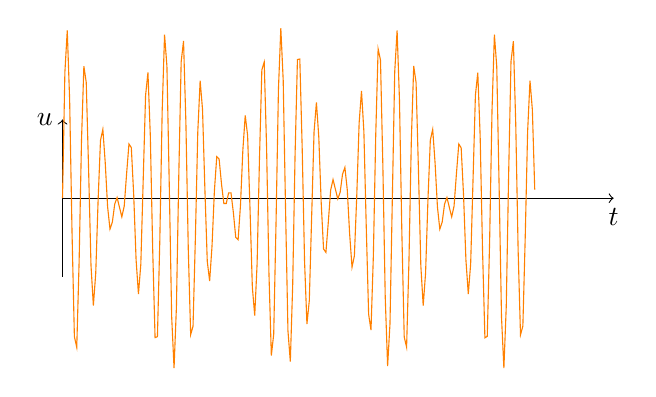
\begin{tikzpicture} 
	\centering
	% draw the axis
	\draw[->] (0,0) -- (7,0) node[below] {$t$};
	\draw[->] (0,-1) -- (0,1) node[left] {$u$};
	\draw[ orange, samples=200,domain=0:6] plot(\x, { (1-0.85^2)^(-1) * (sin( \x r *30 ) + sin (0.85*\x r *30 )      )  *0.3       } );
	\end{tikzpicture} \\
	策动频率与固有频率接近时,出现共振
\end{frame}

\begin{frame}
	\begin{block} {Remark}
	无阻尼强迫振动微分方程一般式为:
	\begin{equation*}
		\frac{d^2 u}{d t^2} + \omega ^2 u = f(t)
	\end{equation*}
	当策动函数为多项式函数,三角函数时, 待定系数法可确定特解。对于其他的情况,一般常采用常数变易法求解。
	\end{block}
\end{frame}

\subsection{常见求解方法}

\begin{frame}
\frametitle{常微分方程求解方法}
	\begin{exampleblock} {例 11、求解一阶常系数线性非齐次常微分方程}
	\begin{equation*}
		y'+py=f(x)
	\end{equation*}
	\end{exampleblock}
	\alert{解、} 对应的齐次方程是衰减数学模型,有解:\\
	\begin{center}
		$w=C_0 exp(-px)$
	\end{center} 
	应用常数变易法,设非齐次方程的解为:\\
	\begin{center}
		$y(x) =u(x) exp(-px)$
	\end{center} 
\end{frame}

\begin{frame}
	\begin{align*}
		y'&= -p u(x) exp(-px) + u'(x) exp(-px)   \\
		py&= p u(x) exp(-px)
	\end{align*}	
	代入原方程得:
	\begin{align*}
		exp(-px)u'(x)&= f(x)\\
		u(x) &= \int exp(px) f (x)dx + C
	\end{align*}
	方程的解为: $ y(x)=C exp(-px)+exp(-px) \int exp(px)f(x)dx $ \\
\end{frame}

\begin{frame}
\begin{exampleblock} {例 12、求解二阶常系数线性常微分方程}
	\begin{equation*}
		y''+py'+qy=f(x)
	\end{equation*}
	\end{exampleblock}
	\alert{解、} 对应的齐次方程为:
	\begin{equation*}
		y''+py'+qy=0
	\end{equation*}
	特征方程为:
	\begin{equation*}
		\lambda^2 +p\lambda +q=0
	\end{equation*}
	解有三种情况:
	\begin{table} [H]
	\begin{tabular}{ccc}
		两相异实根:& $\lambda_1 \ne \lambda_2 $ & \\
		两相同实根:& $\lambda_1 = \lambda_2 $  &\\
		两共轭复根:& $\lambda_1=\alpha+i\beta $, & $\lambda_2=\alpha-i\beta$\\ 
	\end{tabular}
	\end{table}
\end{frame}

\begin{frame}
	对应的齐次方程的通解:
	\begin{table} [H]
	\begin{tabular}{cccc}
		异实根:y=& $C_1 exp(\lambda_1 x)+ C_2 exp (\lambda_2 x) $  \\  
		\\
		同实根:y=&$(C_1+C_2x)  exp (\lambda_1 x) $   \\  
		\\
		共轭复根:y=& $ exp(\alpha x)  [C_1 \cos (\beta x)+ C_2 sin (\beta x)] $\\   
	\end{tabular}
	\end{table}
	根据自由项的特点,再通过待定系数法 或常数变易法求解非齐次常微分方程。
\end{frame}

\begin{frame}
\begin{exampleblock} {例 13、求二阶齐次常微分方程的通解}
	\begin{equation*}
		u''-k^2u'=0
	\end{equation*}
	\end{exampleblock}
	\alert{解、}  特征方程为:
	\begin{equation*}
		\lambda^2 -k^2=0
	\end{equation*}
	存在两相异实根: $\lambda_1=k, ~~ \lambda_2 =-k $ \\    	\vspace{0.3cm}
	通解:~~~~~~~~~u(x)= $C_1 exp(k x)+ C_2 exp (-k x) $  \\  	\vspace{0.3cm}
	写成双曲函数: u(x)= $D_1 cosh(k x)+ D_2 sinh (k x) $  \\
\end{frame}

\begin{frame}
\begin{exampleblock} {例 14、求二阶常微分方程初值问题}
	$\begin{cases}
		u'' =f, (x>0)\\
		u(0)=0, u'(0)=0
	\end{cases}$
	\end{exampleblock}
	\alert{解、} 方程两边求积分
	\begin{equation*}
		u'=\int_{0}^{\xi} f(s) ds +c_1
	\end{equation*}
	\begin{equation*}
		u(x)=\int_{0}^{x}   d\xi  \int_{0}^{\xi} f(s) ds +c_1x  +c_2
	\end{equation*}
	代入零值条件,得  $c_1=0, c_2=0$, 现交换积分次序\\
	\begin{equation*}
		u(x)=\int_{0}^{x}   ds  \int_{s}^{x} f(s) d\xi = \int_{0}^{x}  (x-s)f(s) ds 
	\end{equation*}      
\end{frame}

\begin{frame}
	\begin{exampleblock} {例 15、求二阶常微分方程的初值问题}
	$\begin{cases}
		u'' =f, (x>0)\\
		u(0)=\alpha, u'(0)=\beta
	\end{cases}$
	\end{exampleblock}
	\alert{解、}  显然,$v(x)=\alpha+\beta x$ 是如下齐次方程的解\\
		$\begin{cases}
			u'' =0, (x>0)\\
			u(0)=\alpha, u'(0)=\beta
		\end{cases}$\\
		令 $u(x)=v(x)+w(x)$, 则 w(x) 满足如下零值问题\\	
		$\begin{cases}
			u'' =f, (x>0)\\
			u(0)=0, u'(0)=0
		\end{cases}$\\	  
		由上题可写出原方程的解\\
		\begin{equation*}
			u(x)=\alpha+\beta x + \int_{0}^{x} (x-s)f(s) ds 
		\end{equation*}      
\end{frame}

\begin{frame}
	\begin{exampleblock} {例 16、常数变易法求初值问题}
	$\begin{cases}
		u'' +\omega ^2 u =f, (t>0)\\
		u(0)=0, u'(0)=0
	\end{cases}$
	\end{exampleblock}
	\alert{解、} 齐次方程有通解:
	\begin{equation*}
		u=C_1 \cos(\omega t)+C_2 \sin(\omega t)
	\end{equation*}     
	作常数变易,设非齐次方程的解可写为 
	\begin{equation*}
		u=C_1(t) \cos(\omega t)+C_2(t) \sin(\omega t)
	\end{equation*}    
\end{frame}

\begin{frame}
	求导,得
	\begin{equation*}
		u'=[C'_1(t) \cos(\omega t)+C'_2(t) \sin(\omega t)] + [  - \omega C_1(t) \sin(\omega t)+ \omega C_2(t) \cos(\omega t)  ]
	\end{equation*}    
	令 ~~ [$C'_1(t) \cos(\omega t)+C'_2(t) \sin(\omega t)$] =0,  ~~~ $\dots$  ~~~(1)\\
	\begin{equation*}
		u'= [  - \omega C_1(t) \sin(\omega t)+ \omega C_2(t) \cos(\omega t)  ]
	\end{equation*}    
	二次求导:
	\begin{equation*}
		u''= [  - \omega C'_1(t) \sin(\omega t)+ \omega C'_2(t) \cos(\omega t)  ] -\omega^2 u
	\end{equation*}  
\end{frame}

\begin{frame}
	代回原方程,得:
	\begin{equation*}
		[  - \omega C'_1(t) \sin(\omega t)+ \omega C'_2(t) \cos(\omega t)  ] =f      ~~~~  \left( 2\right)
	\end{equation*}  
	联立(1)(2), 得方程组:\\  	
	$\begin{bmatrix}
		\cos(\omega t) & \sin(\omega t) \\ 
		-\omega \sin(\omega t) & \omega\cos(\omega t)
	\end{bmatrix} $
	$\begin{bmatrix}
		C'_1(t)\\ 
		C'_2(t)
	\end{bmatrix} $ =
	$\begin{bmatrix}
		0\\ 
		f
	\end{bmatrix} $ \\ \vspace{0.3cm}
	解得:\\  
	$\displaystyle \begin{cases}
		C'_1(t)=\dfrac{1}{\omega} \sin(\omega t) f \\ 
		C'_2(t)=\dfrac{1}{\omega} \cos(\omega t) f 
	\end{cases} $ 
\end{frame}

\begin{frame}
	积分得:\\  
	$\displaystyle \begin{cases}
		C_1(t)=\dfrac{1}{\omega} [\int_{0}^{\tau} \sin(\omega \tau) f(\tau)  d\tau +c_1 ]\\ 
		C_2(t)=\dfrac{1}{\omega} [\int_{0}^{\tau} \cos(\omega \tau) f(\tau)  d\tau +c_2 ]\
	\end{cases} $ \\ \vspace{0.3cm}
	方程有解:\\
	\begin{align*}
		u=&\dfrac{1}{\omega}\cos(\omega t)[\int_{0}^{\tau} \sin(\omega \tau) f(\tau)  d\tau +c_1 ] \\
		&+\dfrac{1}{\omega} \sin(\omega t) [\int_{0}^{\tau} \cos(\omega \tau) f(\tau)  d\tau +c_2 ]
	\end{align*} \\ \vspace{0.3cm}
	代入初值条件, 得 $c_1=c_2=0$, 原方程的解:\\
	\begin{equation*}
		u=\frac{1}{\omega}\int_{0}^{\tau} \sin\omega (t-\tau)  f(\tau)  d\tau
	\end{equation*}   
\end{frame}

\begin{frame}
\frametitle{变系数二阶常微分方程}
	\begin{exampleblock} 	{例 17、求解欧拉方程}
	\begin{equation*}
		x^2 \frac{d^2 y}{d x^2} +x \frac{d y}{d x} +n^2 y =0 
	\end{equation*}     
	\end{exampleblock}	
	\alert{解、}  令 $x=exp(t) , (t=ln x)$,求微分:\\
	\begin{equation*}
		\frac{d y}{d x}  = 	\frac{d y}{d t}\frac{d t}{d x}= \frac{1}{ x}\frac{d y}{d t}  \to x \frac{d y}{d x}=	\frac{d y}{d t}
    \end{equation*} 
	\begin{equation*}
		\frac{d ^2y}{d x^2}  = 	\frac{d }{d t} ( \frac{1}{ x}\frac{d y}{d t}  )\frac{d t}{d x}=  
		\frac{1}{ x^2}(\frac{d ^2y}{d t^2} -	\frac{d y}{d t})   \to  	x^2 \frac{d^2 y}{d x^2} = \frac{d ^2y}{d t^2} -	\frac{d y}{d t}
	\end{equation*} 
	代入原方程...
\end{frame}

\begin{frame}
	方程可转化为:
	\begin{equation*}
		\frac{d^2 y}{d t^2}  +n^2 y =0 
	\end{equation*}     
	这是振动方程,有通解:$	y(t)=C_1 \cos n t +C_2 \sin n t$ \\
	代回变量,原方程的解为:
	\begin{equation*}
		y(x)=C_1 \cos (n \ln x) +C_2 \sin (n \ln x)
	\end{equation*}    
\end{frame}

\begin{frame}
	\begin{exampleblock} {例 18、求解如下形式的欧拉方程}
	\begin{equation*}
		x^2 \frac{d^2 y}{d x^2} +2x \frac{d y}{d x} -n(n+1) y =0 
	\end{equation*}     
	\end{exampleblock}
	\alert{解、} 	令 $x=exp(t) , (t=ln x) $, 代入原方程可转化为:
	\begin{equation*}
		\frac{d^2 y}{d t^2}  +\frac{dy}{dt}-n(n+1) y =0 
	\end{equation*}     
	其特征方程为
	\begin{equation*}
		\lambda^2 +\lambda -n(n+1) =0	
	\end{equation*}    
	两相异实根:
	\begin{equation*}
		\lambda_1=n, ~~~\lambda_2= -(n+1)
	\end{equation*}  
\end{frame}

\begin{frame}  
	方程的解为:
	\begin{equation*}
		y(t)=C_1 \exp (nt) +C_2 \exp (-(n+1) t)
	\end{equation*}  
	代回 t=ln x:
	\begin{equation*}
		y(x)=C_1 x^n +C_2 x^{-(n+1) }
	\end{equation*}   
\end{frame}

\begin{frame}
	\begin{exampleblock} {例 18'、求解如下形式的欧拉方程}
	\begin{equation*}
		x^2 \frac{d^2 y}{d x^2} -2x \frac{d y}{d x} +2y = \ln^2( x) -2 \ln(x) 
	\end{equation*}    
	\end{exampleblock}
	\alert{解、} 	令 $x=exp(t) , (t=ln x) $, 原方程可转化为:
	\begin{equation*}
 		\frac{d^2 y}{d t^2}  -3\frac{dy}{dt} +2 y =t^2 -2t 
 	\end{equation*}    
 	这是常系数齐次方程,其特征方程为:
 	\begin{equation*}
 		\lambda^2  -3\lambda +2  =0  \to  \lambda_1=1,   \lambda_2=2 
 	\end{equation*}   
\end{frame}


\begin{frame}
	齐次方程的通解为:
	\begin{equation*}
		y_1=C_1 e^t +C_2 e^{2t}
	\end{equation*}   
	设非齐次方程的特解为:
	\begin{equation*}
		y_2=a t^2+bt+c
	\end{equation*} 
	代回非齐次方程,得特解:
	\begin{equation*}
		y_2=\frac{1}{2} t^2+\frac{1}{2}t+\frac{1}{4}
	\end{equation*} 
	原方程的解为:
	\begin{equation*}
		y(t)=y_1+y_2=C_1 e^t +C_2 e^{2t}+\frac{1}{2} t^2+\frac{1}{2}t+\frac{1}{4}
	\end{equation*} 
\end{frame}


\begin{frame}
	代回$t=ln x $:
	\begin{equation*}
		y(x)=C_1 x +C_2 x^2+\frac{1}{2} \ln ^2 x+\frac{1}{2}\ln x+\frac{1}{4}
	\end{equation*} 
	\begin{block} {Remark}
		变量代换后,再由特征方程写通解是门艺术!
	\end{block}  
\end{frame}

\begin{frame}
	\begin{exampleblock} {例 19、幂级数方法求解 n 阶厄米方程}
	\begin{equation*}
		\frac{d^2 y}{d x^2} -2x \frac{d y}{d x} +2n y =0 
	\end{equation*}     
	\end{exampleblock}	
	\alert{解、} 	设方程有级数解
	\begin{equation*}
		y=\sum_{k=0}^{\infty} c_k x^k
	\end{equation*}     
	求导:\\
	$\begin{cases}
		y' = \sum_{k=1}^{\infty} k c_k x^{k-1} =\sum_{k=0}^{\infty} (k+1) c_{k+1} x^{k}\\
		y'' = \sum_{k=2}^{\infty} k (k-1) c_k x^{k-2} =  \sum_{k=0}^{\infty} (k+2) (k+1) c_{k+2} x^k
	\end{cases}$ \\
    代回原方程:
 \end{frame}

\begin{frame}
	\begin{equation*}
		\sum_{k=0}^{\infty} [ 2nc_k -2kc_k +(k+2)(k+1) c_{k+2}  ] x^k  =0
	\end{equation*}  
	各项系数为零,即: 
	\begin{equation*}
		2nc_k -2kc_k +(k+2)(k+1) c_{k+2} =0
	\end{equation*}   
	得系数递推式:
	\begin{equation*}
		c_{k+2} = \frac{ 2(k-n)}{(k+2)(k+1) } c_k, ~~  \left( k=0,1,2,3, ...  \right)
	\end{equation*}   
	分偶数阶和奇数阶来写,偶数阶有: \\
	$\displaystyle \begin{cases}
		c_2 =- \frac{2n}{2!} c_0\\
		c_4 = \frac{2^2n(n-2)}{4!} c_0 \\
		c_6 = -\frac{2^3n(n-2)(n-4)}{6!} c_0 \\
		c_{2m} = (-1) ^m \frac{2^mn(n-2)(n-4) ... (n-2m+2)  } {(2m)!} c_0
	\end{cases}$ \\
\end{frame}

\begin{frame}	
	同理,奇数阶有:\\
	{ $\displaystyle
		c_{2m+1} = (-1) ^m \frac{2^m (n-1) (n-3)(n-5)...(n-2m+1)  } {(2m+1)!} c_1$}\\ \vspace{0.3cm}
	所有系数求解,即幂级数求得,\\
	$\displaystyle \begin{cases}
		y_1(x)  = [1- \dfrac{2n}{2!} x^2+ \dfrac{2^2n(n-2)}{4!} x^4 -...  ] \\
		y_2(x)  = [x- \dfrac{2(n-1)}{3!} x^3+ \dfrac{2^2(n-1)(n-3) }{5!}x^5 -...  ]
	\end{cases}$ \\ \vspace{0.3cm}
	原方程的解为:
	\begin{equation*}
		y(x) =c_0y_1(x)+c_1 y_2(x).
	\end{equation*}   
\end{frame}

\section{傳里叶级数和傅里叶变换}
\subsection{傳里叶级数 }

\begin{frame}
\frametitle{傳里叶级数}
	\textbf{\large 三角式}:\\
	{\large  $\displaystyle f(x) =\dfrac{a_0}{2} +\sum_{n=1}^{\infty}  \left(  a_n \cos~ \frac{n\pi}{l} x +  b_n \sin~ \frac{n\pi}{l} x  \right) $ }\\	
	{\large $\displaystyle a_n =\frac{1}{l}  \int_{-l}^{l}  f(\xi )   \cos~ \frac{n\pi}{l} \xi d\xi  $ }\\	
	{\large $\displaystyle b_n =\frac{1}{l}  \int_{-l}^{l}  f(\xi )   \sin~ \frac{n\pi}{l} \xi d\xi   $ }\\	
\end{frame}

\begin{frame}
	\textbf{ \large 复数式:} \\  
	{\large  $\displaystyle f(x) =\sum_{n=-\infty}^{+\infty}  c_n e^{i\omega_n x} $ }\\	
	{\large $\displaystyle c_n =\frac{1}{2l}  \int_{-l}^{l}  f(\xi)    e^{-i\omega_n x}  d\xi  $ }\\	
	其中:{\large $\displaystyle   \omega_n=\frac{n\pi}{l} ,  n=...,-3,-2,-1,0,1,2,3,...   $} \\
\end{frame}

\begin{frame}
	\textbf{{\large 周期($2l$) 与 非周期 ($l~\to ~\infty $}}) \\
	{\large  $\displaystyle f(x) =\lim_{l\to \infty} \sum_{n=-\infty}^{+\infty}  c_n e^{i\omega_n x} $ }\\	
	\hspace{5em}{\large $\displaystyle =\lim_{l\to \infty} \sum_{n=-\infty}^{+\infty}  \frac{1}{2l}  [\int_{-l}^{l}  f(\xi)  e^{-i\omega_n x}  d\xi ]  e^{i\omega_n x}  $ }\\	
	\hspace{5em}{\large $\displaystyle =\frac{1}{2\pi} \int_{-\infty}^{+\infty}  [\int_{-l}^{l}  f(\xi)  e^{-i\omega x}  d\xi ]  e^{i\omega x} d\omega $ }\\
	\hspace{5em}{\large $\displaystyle =\frac{1}{2\pi} \int_{-\infty}^{+\infty}  G(\omega) e^{i\omega x} d\omega $ }\\
	\begin{block} {Remark}
		$1, \cos(x), \sin (x), \cos(2x), \sin (2x), ..., \cos(nx), \sin (nx) $, 构成正交完全集,
		$\left\{  exp(i\omega x)  \right\}$  也构成正交完全集。\\
	\end{block}
\end{frame}

\begin{frame}
%\begin{tikzpicture}
%	\draw[->] (0,0) -- (8,0) node[below] {$x$};
%	\draw[->] (0,0) -- (0,4) node[right] {$y$};
%	\draw [blue, thick, x=0.0185cm, y=2cm,
%	declare function={
%		sines(\t,\a,\b,\c,\d,\e )=1 + \a*sin(\t)+\b*sin(\t*\d)+\c*sin(\t*\e));
%	}]
%	plot [domain=0:360, samples=144, smooth] (\x,{sines(\x,0.5, 0.2, 0.1, 3, 5)}); 
%\end{tikzpicture}
	\begin{equation*}
		y=1 + 0.5\sin(x)+0.6\sin(3x)+0.7\sin(5x)
	\end{equation*}    
\end{frame}

\begin{frame}
	\begin{exampleblock} {例20、求函数的傳里叶展开式}
	$\displaystyle f(x)=\begin{cases}
		1 , ~~~ x \in [0, \pi] \\
		-1 ,~~~ x \in [-\pi, 0] \
	\end{cases}$ \\
	\end{exampleblock}
	\alert{解、} 这是个奇函数, 展开式中只有$sin$函数, 计算 $b_n$\\
	\begin{align*}
		b_n &=\frac{1}{\pi}  \int_{-\pi}^{\pi}  f(x) \sin~ \frac{n\pi}{\pi} x dx  \\	
		&=\frac{1}{\pi}  [ \int_{-\pi}^{0}  \sin n x dx - \int_{0}^{\pi}  \sin~nx dx] \\
		&=\frac{2}{\pi}  \int_{0}^{\pi}  \sin nx dx  \\
		&=\frac{2}{n\pi} [\cos nx] |_0 ^\pi =\frac{2}{n\pi} [ (-1) ^n -1]
	\end{align*}
\end{frame}

\begin{frame}
	得傳里叶展开式:
	\begin{equation*}
		f(x) = \frac{4}{\pi} \sum_{n=0}^{\infty}  \frac{1}{2k+1} \sin(2k+1) dx  
	\end{equation*}       
\end{frame}

\subsection{傳里叶变换 }

\begin{frame}
\frametitle{傳里叶变换 }
	由非周期的傳里叶级数,获得傳里叶变换公式:\\
	$\displaystyle \begin{cases}
		G(\omega) =\int_{-\infty}^{+\infty}  f(x) e^{-i\omega x} dx \\
		f(x) =\dfrac{1}{2\pi} \int_{-\infty}^{+\infty}  G(\omega) e^{i\omega x} d\omega
	\end{cases}$ \\ \vspace{0.3cm}
	{对称形式:}\\ 
	$\displaystyle \begin{cases}
		G(\omega) =\dfrac{1}{\sqrt{2\pi}} \int_{-\infty}^{+\infty}  f(x) e^{-i\omega x} dx  \equiv F[f(x)]\\
		f(x) =\dfrac{1}{\sqrt{2\pi}}  \int_{-\infty}^{+\infty}  G(\omega) e^{i\omega x} d\omega  \equiv F^{-1}[G(\omega)]
	\end{cases}$ \\	
\end{frame}

\begin{frame}
	\frametitle{}
	{\large   物理意义  }\\ 	\vspace{0.3cm}
	{\Large   $\displaystyle f(x) =\frac{1}{\sqrt{2\pi}}  \int_{-\infty}^{+\infty}  G(\omega) e^{i\omega x} d\omega $ }\\	\vspace{0.3cm}
    一个复杂时域信号总是由各种频域的波叠加形成!	\\ \vspace{0.3cm}
	tips: 一种数学物理方法的成功不是由于巧妙的谋略或者幸运的偶遇,而是因为他表达着物理真理的某个方面 ~~~~~~-------沙顿
\end{frame}

\begin{frame}
	\frametitle{}
	{\large   性质  }\\ 	\vspace{0.3cm}
    线性: $F[\alpha  f_1 +\beta f_2]=\alpha  F[f_1]+ \beta F[f_2]$ \\ \vspace{0.3cm}
    延迟: $F[e^{i\omega_0x} f(x)] = G(\omega-\omega_0) $ \\ \vspace{0.3cm}
    位移: $F[ f(x\pm x_0)] = e^{i\omega x_0 } F[f(x)]=e^{i\omega x_0 }G(\omega) $ \\ \vspace{0.3cm}
    相似: $F[ f(\alpha  x)] = \frac{1}{|\alpha |}G(\frac{\omega}{\alpha }) $ \\ \vspace{0.3cm}
    微分: $F[ f^{n} (x)] = (i\omega ) ^n F[f(x)]= (i\omega )^n G(\omega) $ \\ \vspace{0.3cm}
    积分: $F[ \int_{x_0}^{x}f (\xi) d\xi ] = \frac{1}{\omega}  F[f(x)]=\frac{1}{\omega} G(\omega) $ \\ \vspace{0.3cm}
\end{frame}

\begin{frame}
	\begin{exampleblock} {例 21、求动量表象波函数}
	{在量子力学中,一维体系在坐标表象中的波函数如下,求在动量表象中的波函数 $c(p)$}
		\begin{equation*}
			\Psi(x)=\frac{1}{\sqrt{2\pi \hbar}}  \int_{-\infty}^{+\infty} c(p) e^{\frac{i}{\hbar} px} dp 
		\end{equation*}   	
	\end{exampleblock}
	\alert{解、} 	把波函数改写成  \\	
	\begin{equation*}
		\Psi(x)= \frac{1}{\sqrt{2\pi }} \int_{-\infty}^{+\infty} \sqrt{\hbar} c(p) e^{i\frac{p}{\hbar} x} d(\frac{p}{\hbar})  
	\end{equation*}     
	根据对称型傅里叶变换公式,有: 
	\begin{equation*}
		\sqrt{\hbar} c(p) = \frac{1}{\sqrt{2\pi }} \int_{-\infty}^{+\infty} \Psi(x) e^{-i\frac{p}{\hbar} x} dx
	\end{equation*}   
\end{frame}

\begin{frame}
	得解:
	\begin{equation*}
		c(p) = \frac{1}{\sqrt{2\pi \hbar }} \int_{-\infty}^{+\infty} \Psi(x) e^{-\frac{i}{\hbar} px} dx
	\end{equation*}   
\end{frame}

%\subsection{作业}

\begin{frame}
\frametitle{作业 }
	1、求函数的傳里叶展开式:
	$\displaystyle f(x)=\begin{cases}
		\pi +x , ~~~ x \in [-\pi, 0] \\
		\pi -x ,~~~ x \in   [0, \pi] 
	\end{cases}$ \\
	2、分离变量法求方程\\
	\begin{equation*}
		\frac{dy}{dt}	=  r y (1-\frac{y}{K}), ~~~~ y(t_0) = y_0
	\end{equation*}
	3、	幂级数方法求解方程\\
	\begin{equation*}
		\frac{d^2 y}{d x^2} -2x \frac{d y}{d x} +2n y =0 
	\end{equation*}     
\end{frame}

\begin{frame}
	\frametitle{课外读物和思考}
	\begin{itemize}
		\item 为什么微分方程是线性方程?
		\item 什么是齐次微分方程的辅助方程 ?
		\item 微分方程的解为什么总与exp指数相关? 
		\item 为什么非齐次方程的解由齐次方程的解加特解确定?
	\end{itemize}	
\end{frame}

\begin{frame}
	\alert{说明:} 	定义微分算子 D
	\begin{equation*}
		D= \dfrac{d}{dx}
	\end{equation*}	
	定义线性算子 T
	\begin{equation*}
		T(a f(x) +b g(x) )  =a T(f(x)) +b T(g(x)) 
   \end{equation*}	
 	利用f(x) 和g(x)的Taylor 展开式,很容易证明微分算子 D是线性的。\\
	微分算子多项式$	L= c_0 + c_1D +c_2D^2 +...  $也是线性算子。\\
\end{frame}

\begin{frame}
    定义微分方程:
    \begin{equation*}
    	L(y)=f(x)
    \end{equation*}
    若{ $c_0$} 都是常数,称为常系数微分方程,否则称为变系数微分方程。 称$L(y)=0$为齐次方程, 	$L(y)=f(x)\ne0$为非齐次方程。 可以证明常系数微分方程是线性的,如果$y_1(x) ,  y_2(x) $是方程的解,则它们的线性叠加
    \begin{equation*}
    	y(x)=c_1y_1(x) +c_2y_2(x) 
    \end{equation*}	
    也是方程的解。
\end{frame}

\begin{frame}	
	微分算子 D的特征方程有解
	\begin{equation*}
		D(e^{nx})=n e^{nx}
	\end{equation*}	
	n 是特征值($\lambda=n$),$e^{nx}$ 属于 n 的特征矢。\\
	对于算子$L= c_0 + c_1D +c_2D^2 $,特征值为$\lambda=c_0 + c_1n +c_2n^2$ \\
	解辅助方程
	\begin{equation*}
		c_2n^2+c_0 + c_1n =0
	\end{equation*}	
	相当于求L算子特征值为零的特征矢,特征矢的线性叠加正是 L(y)=0 这个齐次方程的解。
\end{frame}

\begin{frame}
	对于非齐次方程,先求得齐次方程的解,再由初始条件确定一特解。相当于辅助方程
\end{frame}

%%%%%%%%%%%%%%%%%%%%%%%%%%%%%%%%%%%%55%%
\begin{frame} [plain]
    \frametitle{}
    \Background[1] 
    \begin{center}
    { {\huge 第二章、波函数和薛定谔方程}}
    \end{center}  
    \addtocounter{framenumber}{-1}   
\end{frame}
%%%%%%%%%%%%%%%%%%%%%%%%%%%%%%%%%%

\section{1.波函数}

\subsection{波粒二象性导致的困境}

\begin{frame}
    \frametitle{}
    \begin{tcolorbox4}[前情回顾]
        Wave-particle duality is the inherent attribute of matter\\
        ~~\\
        How to interpret a world where waves are particles and particles are waves
    \end{tcolorbox4}
\end{frame}

\begin{frame}
    \begin{center}
        \includegraphics[width=0.6\textwidth]{figs/Etwoslitexp.png} \\
        \includegraphics[width=0.6\textwidth]{figs/two-slit.png} \\
    \end{center} 
\end{frame}

\begin{frame}
    \frametitle{}
    实验分析:\\
    \begin{itemize}
        \Item 多个波构成电子 
        \Item 多个电子构成 
        \Item 单个电子既是粒子又是波 
    \end{itemize}
\end{frame}

\begin{frame}
    如果单个电子既是粒子又是波 \\
\begin{itemize}
    \Item  电子与自己干涉 
    \Item  电子同时过两个缝  
    \Item  电子至少同时有两条路径 
    \Item  牛顿力学失效! 
    \Item  波动学失效! 
\end{itemize}
\end{frame}

\begin{frame}
    \centering
    \begin{tcbb}[0.68]{波粒二象性导致的困境}
        {如何描述象电子这样具有波粒二象性物体的运动?}
    \end{tcbb}
\end{frame}

%%%%%%%%%%%%%%%%%%%%%
\subsection{波函数假说}
%%%%%%%%%%%%%%%%%%%%%

\begin{frame}
    \frametitle{波函数假说}
    \begin{tcolorbox4}[Basic assumption 1/5]
    In 1924, De Broglie assumed that:\\
    ~\\
    The state of matter is described by a wavefunction \\
    ~\\
    (物体的状态用波函数描述)
    \end{tcolorbox4}
\end{frame}

\begin{frame}
    \frametitle{}
    构造第一个波函数(平面波函数):~\\
    For the classical plane wave,
        \begin{equation*}
            \begin{split}
                y(x,t)&=A e^{i(\frac{2\pi}{\lambda}x-\omega t)} \\
                    & = A e^{i\frac{2\pi}{h}(\frac{h}{\lambda}x-h\nu t)}
            \end{split} 
        \end{equation*}
        Put De Broglie relationship into the formula, we get a quantum plane wavefunction
        \begin{equation*}
            \begin{split}
                \Psi_p(x,t)&=A e^{\frac{i}{\hbar}(px-Et)}
            \end{split} 
         \end{equation*}
         It describes the state of a quantum free particle\\
         \Note ~ A wavefunction is a complex function 
\end{frame}

\begin{frame}
         For a general wavefunction, it should be a wave-packet of plane wavefunction
         \begin{equation*}
                \Psi(x,t)=\sum\limits_{p} c(p)\Psi_p(x,t) = \int\limits_{-\infty} ^{\infty} c(p,t) e^{\frac{i}{\hbar}px}dp
         \end{equation*}
\end{frame}


\begin{frame}
    \frametitle{德布罗意}
        \begin{columns}
            \begin{column}[t]{0.46\linewidth}
                主要成就:\\
                \begin{enumerate}
                    \Item 物质波假说
                    \Item 原子内电子的波动性
                    \Item 波函数假说 
                    \Item 构造第一个波函数
                \end{enumerate}
                ~\\
                \begin{quote}
                "德布罗意已经揭开了面纱的一角"  \\
                    \rightline{$\cdots$ 爱因斯坦 (1925)\hspace{3em}}
                \end{quote}  
            \end{column}
            \begin{column}[t]{0.46\linewidth}
                \begin{center}
                    \includegraphics[width=0.85\textwidth]{figs/2021-12-03-18-00-05.png} \\
                \end{center} 
            \end{column}
        \end{columns}
\end{frame}

%%%%%%%%%%%%%%%%%%%%%%%%%%%%%%%%%
\section{2.波函数统计诠释}
%%%%%%%%%%%%%%%%%%%%%%%%%%%%%%%%%

\subsection{统计诠释}
\begin{frame}
    \frametitle{统计诠释}
    In 1926, Born proposed statistical interpretation of wavefunction
    \begin{tcolorbox4}[Statistical interpretation]
        \large The magnitude of wavefunction $\Psi(\vec{r},t)$ does not tell us how much of 
        the particle is at position $\vec{r}$ at time t, 
        but rather the probability (W) that the particle is at or near the position at time t. \\
        \[ d W = |\Psi(\vec{r},t)|^2 d \tau \]
    \end{tcolorbox4}
    {\color{deepred} Nobel Prize in physics(1954)}
\end{frame}

\begin{frame}
    \frametitle{}
    解释干涉实验:
    \begin{itemize}
        \Item 自由电子是平面波,可等概率出现在屏的任一位置
        \Item 电子波通过双缝发生衍射和干涉,导致某些位置的振幅大,某些位置的振幅小
        \Item 振幅较大的位置电子出现的概率大,形成明纹。振幅小的位置电子出现的概率小,形成暗纹
        \Item 明暗干涉条纹不体现电子波的形状,体现的是电子出现概率的分布
    \end{itemize}  
\end{frame}

\subsection{统计诠释的数学描述}

\begin{frame}[allowframebreaks=]
    统计诠释的数学描述:
    \begin{enumerate}
        \Item Probability density \[\omega = |\Psi|^2 =\Psi^* \Psi \]
        \Item Probability  \[ d W = |\Psi|^2 d \tau \]
        \Item Normalization \[ \int_{\Omega} |\Psi|^2 d \tau =1 \]
        \Item Momentum wavefunction \[ c(\vec{p},t)=\frac{1}{(2\pi\hbar)^{3/2}} \int_{-\infty}^{\infty} \Psi(\vec{r},t) e^{\frac{-i}{\hbar} \vec{p}\cdot \vec{r} } d \tau \] 
        \Item Expectation value of any function $f (x)$  \[ <f(x)>=\int_{-\infty}^{\infty} f(x) |\Psi(x)|^2 dx \]
        \Item Expectation value of observable A \[ <A>=\int_{-\infty}^{\infty} \Psi^*(x) [A \Psi](x)| dx \]
    \end{enumerate}
\end{frame}

\begin{frame}
    \frametitle{}
    \Tips \\
    \begin{itemize}
        \Item $\Psi$ and $C\Psi$ describe the same state 
        \[ \frac{C\Psi(x_1)}{C\Psi(x_2)} = \frac{\Psi(x_1)}{\Psi(x_2)}\]
        \Item $\Psi$ and $e^{i\varphi}\Psi$ describe the same state 
         \[ |e^{i\varphi}\Psi|^2 = e^{-i\varphi} e^{i\varphi} |\Psi|^2 = |\Psi|^2 \] 
    \end{itemize}  
    * 两相同的波叠加, 在测量上并没有什么不同,与经典条件下两相同的波叠加完全不同
\end{frame}

\begin{frame}
    Statistical interpretation requires wavefunctions to be (标准化条件):
    \begin{itemize}
        \Item finite  function
        \Item continuous function 
        \Item monotropic function
        \Item square integrable function 
    \end{itemize}
\end{frame}

\begin{frame}[allowframebreaks=]
    \frametitle{}
    \EXP[1.~normalizating the wavefunction] {\[\psi(x)=\sin(x), \qquad (0\le x \le \pi)\]}
    \Solution ~assuming the normalized wavefunction to be 
    $\Psi=C\sin(x)$
    \begin{equation*}
        \begin{split}
            \int_0 ^\pi |C\sin(x)|^2 dx &=1 \\
            C^2 \int_0 ^\pi \sin^2(x) dx &=1 \\
            C^2 \int_0 ^\pi \frac{1-\cos 2x }{2} dx &=1 \\ 
            C^2 [\frac{x}{2}-\frac{\sin 2x}{4}]_0 ^\pi &=1 \\ 
        \end{split} 
     \end{equation*}
     \[C=\sqrt{\frac{2}{\pi}}\]
     The normalized wavefunction:
     \begin{equation*}
        \Psi=C\sin(x)=\sqrt{\frac{2}{\pi}}\sin(x)
    \end{equation*}
\end{frame}

\begin{frame}[allowframebreaks=]  
    \EXP[2.~normalizating the plane wavefunction ] {\[\Psi_p (x,t)=e^{\frac{i}{\hbar}(px-Et)} \] }
    \Solution  ~assuming the normalized wavefunction 
    $\Psi=C\Psi_p (x,t)$
    \begin{equation*}
        \begin{split}
            \int_{-\infty} ^\infty |C\Psi_p (x,t)|^2 dx &=1  \\
            C^2 \int_{-\infty} ^\infty \Psi_p (x) \Psi_{p} ^* (x) dx &=1  \\
            C^2 \int_{-\infty} ^\infty \Psi_p (x) \Psi_{p'} ^* (x) dx &=\delta (p-p')  \\
            C^2 \int_{-\infty} ^\infty e^{\frac{i}{\hbar}(p-p')x} dx &=\delta (p-p')\\
        \end{split} 
     \end{equation*}
     with the defination of $\delta$ funcation,
     \[ \delta(x)=\int_{-\infty}^{+\infty} \frac{d k}{2 \pi} e^{i k x}\]
     we get
     \[C^2 2\pi \hbar \delta (p-p') =\delta(p-p') \]
     \[C= \dfrac{1}{\sqrt{2\pi \hbar}}\]
     The normalized plan wavefunction:
     \begin{equation*}
        \Psi=\frac{1}{\sqrt{2\pi \hbar}} e^{\frac{i}{\hbar}px}
    \end{equation*}  
    In general
    \[ \Psi(\vec r ,t)=\frac{1}{(2\pi \hbar)^{3/2}} e^{\frac{i}{\hbar}(\vec p\cdot \vec r -Et)} \]
    \[ \Psi(\vec r_1 ,\vec r_2, t)=\frac{1}{(2\pi \hbar)^{6/2}} e^{\frac{i}{\hbar}(\vec p_1 \cdot \vec r_1 +\vec p_2 \cdot \vec r_2 -Et)} \]
\end{frame}

\begin{frame}
    \frametitle{玻恩 (Max Born)}
        \begin{columns}
            \begin{column}[t]{0.46\linewidth}
                主要成就:
                \begin{enumerate}
                    \Item 波函数的统计诠释
                    \Item 态叠加原理
                \end{enumerate}
                德国理论物理学家,量子力学的奠基人之一。\\
                因对波函数的统计解释,获1954年诺贝尔物理学奖.\\
                1912年受聘哥廷根大学无薪讲师,1933年因犹太血统被剥夺教职和财产,流亡英国.\\ \vspace{0.3em}
                泡利、海森堡和黄昆都是他的学生
            \end{column}
            \begin{column}[t]{0.46\linewidth}
                \begin{center}
                    \includegraphics[width=0.9\textwidth]{figs/Born.png} \\
                \end{center} 
            \end{column}           
        \end{columns}
\end{frame}

\begin{frame}  
    \begin{tcolorbox3}[Conclusion]
        ~~\\
       {The state of matter is described by a wavefunction and the magnitude of the wavefunction $ \Psi(x,t)$ 
       tells us the probability that the particle is at or near the position ($x$) at time $t$.}
    \end{tcolorbox3} 
\end{frame} 

\begin{frame}
    \frametitle{}
    \centering
    \tcbb[0.5]{Big problems}
    {
    {Is the world obeys the rule of probability ?}
    }
\end{frame}
 %%%%%%%%%%%%%%%%%%%%%%%%%%%%%%%%%%%%%%%%%%%%%%%%%%%%%%%%%%%%%%%%%%%
 \begin{frame}
     \frametitle{课外作业}
     \begin{enumerate}
        \item 已知氢原子电子的波函数(t=0)为$\psi(r)=Ae^{-r/a_0} $,试求:\\
               (1) 归一化系数A \\
               (2) 电子在$r-r+dr$之间出现的概率\\
               (3) 电子在哪里出现概率最大(r的值) 
        \item 已知氢原子电子的波函数(t=0)为$ Y_{10} $,试求:\\
                (1) 电子在$(\theta, \varphi) -(\theta + d \theta, \varphi + d \varphi)$之间出现的概率\\
                (2) 电子在哪个方位出现的概率最大 
     \end{enumerate}
 \end{frame}
 %%%%%%%%%%%%%%%%%%%%%%%%%%%%%%%%%%%%%%%%%%%%%%%%%%%%%%%%%%%%%%%%%%%

 \section{3.态叠加原理}

 \begin{frame}
     \frametitle{前情回顾}
     \begin{itemize}
         \Item 波粒二象性
         \Item 波函数假说
         \Item 波函数统计诠释
     \end{itemize}
 \end{frame}  
 
 \subsection{态叠加原理实验基础}
 
 \begin{frame}
     \frametitle{两种双缝实验}
         \begin{figure}
             \centering
             \subfigure[小球双缝实验]{\includegraphics[width=0.49\textwidth]{figs/2022-01-17-13-50-38.png}}
             \subfigure[电子双缝实验]{\includegraphics[width=0.49\textwidth]{figs/2022-01-17-13-51-15.png}}
         \end{figure}
     \setcounter{subfigure}{0}
 \end{frame}
 
 \begin{frame}
     \frametitle{小球双缝实验}
     \begin{center}
         \includegraphics[width=0.5\textwidth]{figs/sup-2.png} \\
     \end{center} 
     依据统计诠释,振幅是概率幅\\
     \begin{itemize}
         \Item 小球双缝实验,$P'=P_1+P_2 $, 是概率叠加。
         \Item 结论:经典叠加服从概率叠加
     \end{itemize}
 \end{frame} 
 
 
 \begin{frame}
     \frametitle{电子双缝实验}
     \begin{center}
         \includegraphics[width=0.5\textwidth]{figs/sup-3.png} \\
     \end{center} 
     依据统计诠释,振幅是概率幅\\
     \begin{itemize}
         \Item 电子双缝实验,$P\neq P_1+P_2 $,量子叠加服从的不是概率叠加!
         \Item 波恩认为服从波函数(态)叠加,即:
         $$ \psi =\psi_1+\psi_2$$
     \end{itemize}
 \end{frame} 
 
 
 \begin{frame} [allowframebreaks=]
     \tikzstyle{na} = [baseline=-.5ex]
     Analysing the two-slit experiment:\\
     \begin{itemize}
         \Item Using wavefunction $\psi_1$ to describe the state of the electron running across slit-1 and $\psi_2$ for slit-2. \\
         \Item when the both slits opened, one can assume that the electron locates at the superposition state
             \[ \Psi=c_1 \psi_1+ c_2\psi_2 \]
         \Item based on statistical interpretation, the possiblity density of electron reaches certain point of screen should be
         \begin{equation*}
         \begin{split}
             \omega &=|\Psi|^2 \\
             &= (c_1 \psi_1+ c_2\psi_2)^* (c_1 \psi_1+ c_2\psi_2) \\
             &=(\psi_1^*+\psi_2^*)(\psi_1+\psi_2) \\ 
             & = |c_1|^2 |\psi_1|^2 + |c_2|^2 |\psi_2|^2  
             + \Myitem{t1}{red}{[c_1 c_2 ^* \psi_1 \psi_2 ^* + c_1 ^* c_2 \psi_1 ^* \psi_2]} \\
         \end{split} 
         \end{equation*}
     \end{itemize}
     \begin{itemize}
         \Item 概率计算表明,电子处于叠加态时,存在干涉项(后两项),产生干涉条纹
         \Item 如果电子不处于叠加态,即电子只过一个缝,则有$\psi_1$ 或$\psi_2$为零,不存在干涉项,没有干涉条纹!
         \Item 干涉条纹正是源于电子同时过两个缝的状态, 即叠加态。
     \end{itemize}
     基于此,波恩提出了态叠加原理
 \end{frame}
 
 \subsection{态叠加原理表述}
 
 \begin{frame}
     \frametitle{态叠加原理}
     Born also proposed that: \\
     \begin{tcolorbox4}[Superposition principle of states]
     If $\psi_1$ and $\psi_2$ are the possible states of the system,
     their linear superposition \[ \Psi=c_1 \psi_1+ c_2\psi_2 \]
     is also the possible state of the system.\\
     if the system locates at the superposition $\Psi$, the possiblity of observating the system at $\psi_1$ is $|c_1|^2$, and at $\psi_2$ is $|c_2|^2$ \\
     \[|c_1 |^2 + |c_2 |^2 =1\]
     \end{tcolorbox4}
 \end{frame}
 
 \begin{frame}
     \frametitle{}
     \begin{tcolorbox4}[态叠加原理中文表述]
     如果 $\psi_1$ 、 $\psi_2$、 $\cdots$、$\psi_N$ 是粒子可能的态,那么它们的线性叠加
         $$ \Psi=c_1 \psi_1+ c_2\psi_2+\cdots+c_N\psi_N $$
     也是粒子可能的态(叠加态)\\   
     如果粒子处于叠加态 $\Psi=\sum\limits_{i=1}^N c_i \psi_i$,  
     那么测得粒子处在第$i$态 ($\psi_i$) 的概率为 $|c_i |^2$, 
     并且有  $$\sum_{i=1}^{N} |c_i|^2 =1$$
     \end{tcolorbox4}
     ~~\\ 
     * 经典叠加物体并不部分地处于原来各波的状态,测量时也得到原来各波的值!
 \end{frame}
 
 \subsection{波函数坍塌}
 
 \begin{frame}
     \frametitle{实验升级}
     \begin{center}
         \includegraphics[width=0.5\textwidth]{figs/sup-4.png} \\
     \end{center} 
     \begin{itemize}
         \Item 目标:观测电子是如何同时过两条缝的
         \Item 结果:1)只能测到电子要么过第一缝,要么过第二缝。\\
         2)探测器越灵敏,干涉条纹越模糊,\\
         3)当探测器能长时间地保持几乎可以完全判断电子过哪条缝时,干涉条纹消失!如图(b)所示
     \end{itemize}
 \end{frame}
 
 \begin{frame} 
     \frametitle{结果分析}
     \begin{enumerate}
         \Item 实验目标与实验结果的一致性\\
         \begin{itemize}
             \IItem 当我们“挖出”A和B两条狭缝时,“设计”了一个想要观察“波动性”的设备,也就是电子已经预先被我们设定为“波”,因此观测到波动性(干涉条纹)
             \IItem 当我们装上侦测器时,整个实验被我们“设计”成观察“粒子性”,因为想要知道电子到底是由A还是B穿过,就必须先具备确定的“位置”,因此观察到粒子性(干涉条纹消失)
         \end{itemize}
         \Item 测量可导致状态改变\\
         \begin{itemize}
             \IItem 探测前,电子处于叠加态($ \psi =\psi_1+\psi_2$)
             \IItem 探测时,电子状态改变,被迫从叠加态变为确定态 ($\psi_1$ or $\psi_2$),(称为波函数坍塌)
             \IItem 探测后,电子处于某确定态,不能干涉。
             \IItem 探测器不灵敏,有部分没有被探测到的电子处于叠加态, 干涉条纹模糊。
             \IItem 探测器灵敏,全部电子被探测,没有电子处于叠加态, 干涉条纹消失。
         \end{itemize}
     \end{enumerate}
 \end{frame}
 
 \begin{frame}   
     \begin{enumerate}
         \Item 测量结果的互补性(互补性原理)\\
         \begin{itemize}
             \IItem 波动性和粒子性是两种不同的属性,一般不能用同一设备进行测量
             \IItem 不能因为测得粒子性就否定波动性,反之亦然。
             \IItem 测量结果就算相互矛盾,也要同时接受,因为它们互补地揭示物体的本质。
         \end{itemize}
         \Item 结论
         \begin{itemize}
             \IItem 电子具有波粒二象性,总是处于叠加态
             \IItem 不被测量,则保持在叠加态
             \IItem 测量导致确定态,但结果是随机的。
             \IItem 测得电子过某条缝,不能说明电子原本就要过这条缝,为只是测量导致的结果
         \end{itemize}
     \end{enumerate}
 \end{frame}
 
 \subsection{学术大讨论}
 \begin{frame}
     \frametitle{学术大讨论}
     The probabilistic interpretation was controversial from the beginning of of quantum mechanics
     \begin{tcolorbox4}[Which Way?]
     \begin{itemize}
         \Item De Broglie : Pilot waves
         \Item Schr$\ddot{o}$dinger: Schr$\ddot{o}$dinger's cat
         \Item Einstein: EPR paradox
         \Item Wheeler's delayed choice experiment
         \Item Quantum eraser experiment
         \Item $\cdots \cdots$
     \end{itemize}
     \end{tcolorbox4}
 \end{frame}
 
 \begin{frame}
     \frametitle{薛定谔的猫}
     \begin{center}
         \includegraphics[width=0.9\textwidth]{figs/2022-03-04-13-49-09.png} \\
     \end{center} 
 \end{frame}
 
 \begin{frame}
     \frametitle{EPR佯谬}
     \begin{center}
         \includegraphics[width=0.9\textwidth]{figs/28.png} \\
     \end{center} 
 \end{frame}
 
 \begin{frame}
     \frametitle{贝尔不等式}
     \begin{center}
         \includegraphics[width=0.8\textwidth]{figs/bell.png} \\
     \end{center} 
 \end{frame}
 
 \begin{frame}
     \frametitle{惠勒延迟选择实验}
     \begin{center}
         \includegraphics[width=0.7\textwidth]{figs/choose.png} \\
     \end{center} 
 \end{frame}
 
 \begin{frame}
     \frametitle{量子擦除实验}
     \begin{center}
         \includegraphics[width=0.7\textwidth]{figs/c1.png} \\
     \end{center} 
 \end{frame}
 
 \begin{frame}
     \frametitle{}
     \begin{center}
         \includegraphics[width=0.6\textwidth]{figs/c2.png} \\
     \end{center} 
 \end{frame}
 
 \begin{frame}
     \frametitle{}
     \begin{center}
         \includegraphics[width=0.6\textwidth]{figs/c3.png} \\
     \end{center} 
 \end{frame}
 
 \begin{frame}
     \begin{tcolorbox4}[Conclusion]
         ~~\\
     \begin{enumerate}
         \Item Objects are wave-particles and in superposition state
         \Item Measurement changes the state and gives random results
         \Item Measurement results are complementary
         \Item Measurement leads to objective reality
     \end{enumerate}
     \end{tcolorbox4}
 \end{frame}
 
 \begin{frame}
     \frametitle{}
     \centering
     \tcbb[0.5]{Big problems}
     {
       \large  {The world is not a real world?\\
       What is the measurement? \\
       If not performing measurement, what it should be?}
     }
 \end{frame}
 
  %%%%%%%%%%%%%%%%%%%%%%%%%%%%%%%%%%%%%%%%%%%%%%%%%%%%%%%%%%%%%%%%%%%
  \begin{frame}
     \frametitle{课外作业}
     \begin{enumerate}
        \item 已知粒子的波函数(t=0)如下,
            \[\psi(x) = \begin{cases}
              \sqrt{A}\sin \frac{\pi x}{a}, \quad 0\leq x\leq a\\
              0, \qquad  x<0, x>a
            \end{cases}\]
                (1)试求归一化系数A \\
                (2)试求位置的概率密度 \\
                (3)试求动量的概率密度
        \item 试用态叠加原理解释电子双缝干涉实验
     \end{enumerate}
 \end{frame}
 %%%%%%%%%%%%%%%%%%%%%%%%%%%%%%%%%%%%%%%%%%%%%%%%%%%%%%%%%%%%%%%%%%%
 

\section{4.薛定谔方程}

\begin{frame}
    \frametitle{前情回顾}
    \begin{itemize}
        \Item 波粒二象性
        \Item 波函数假说
        \Item 波函数统计诠释
        \Item 态叠加原理
    \end{itemize}
\end{frame}  

\begin{frame}
    \begin{tcolorbox4}[Conclusion]
        ~~\\
    \begin{enumerate}
        \Item Objects are wave-particles and in superposition state
        \Item Measurement changes the state and gives random results
        \Item Measurement results are complementary
        \Item Measurement leads to objective reality
    \end{enumerate}
    \end{tcolorbox4}
\end{frame}  

\begin{frame}
    \centering
    \tcbb[0.5]{Big problems}
    {
      If not performing measurement, what it would be? 
    }
\end{frame}

\subsection{波函数演化假说}

\begin{frame}
    \begin{tcolorbox4}[Basic assumption 2/5]
        The evolution of wavefunction obeys Schr$\ddot{o}$dinger equation
        \begin{equation*}
            i\hbar \frac{\partial }{\partial t} \Psi (\overrightarrow{r},t ) =\left [ -\frac{\hbar^2}{2\mu }\nabla ^2 + V(\overrightarrow{r},t ) \right ]\Psi (\overrightarrow{r}, t ) 
        \end{equation*}
    \end{tcolorbox4}
\end{frame}

\subsection{薛定谔方程}

\begin{frame}
    \frametitle{神秘来源}
    \begin{itemize}
        \Item 1923年,德布罗意博士论文传到了瑞士,一战炮兵指挥官苏黎世大学讲师薛定谔作了一个关于物质波假说的报告,德拜评注:\\
        $$\text{“有了波,总得有个波动方程吧”}$$
        \Item 1926年,薛定谔:
        $$“Dear~Debye, I~find~one~\cdots”$$
    \end{itemize}            
\end{frame}

\begin{frame}
    \begin{alertblock} {}  
    \begin{quote}
        “是粒子还是波?是妻子还是情人?这都是难题!” \\
        ~~\\
        \rightline{--《薛定谔的女友》(2001)\hspace{6em}}   
    \end{quote}  
    \begin{quote}    
    这部话剧讲述了薛定谔方程建立的神秘过程:在1925年圣诞节前,薛定谔像往年一样,来到阿尔卑斯山度假。这次陪伴他的不是妻子安妮,而是维也纳的一位神秘女郎。
    就是这位比薛定谔的猫还神秘的女郎激发了薛定谔的灵感,使他在一年的时间里连发~6~篇~“SCI”~论文,建立波动量子力学,$\cdots$\\
    ~~\\
    \end{quote} 
    \end{alertblock}   
\end{frame}

\begin{frame}
	\begin{alertblock} {可能思路}  
		\begin{itemize}
			\Item 	\textbf{1:}  最小作用量原理 $\int\limits_{t_1}^{t_2} \delta L d t =0 $\\ 
			\Item 	\textbf{2:}  波粒二象性\\ 
			~\\ 
			\Item 	\textbf{3:}  基本假设,不能从现有理论推导\\
            ~\\ 
            \begin{quote}
            "It is not possible to derive it from anything you know. It came out of the \alert{\faHeartbeat} of Schr$\ddot{o}$dinger"\\
            \rightline{$\cdots$ R. P. Feynman \hspace{3em}}   
            \end{quote}
		\end{itemize}
	\end{alertblock}
\end{frame}

\begin{frame} [allowframebreaks=]
    \frametitle{}
    \alert{\faHeartbeat} Quantum plane wavefunction \[\psi(x,t)=\Psi_p(x,t)=e^{\frac{i}{\hbar}(p\cdot x-Et)} \]
    should be a sulotion of this equation
    \begin{equation*}
        \begin{split}
       -i\hbar \nabla \psi(x,t) &=p\psi(x,t) \\ \vspace{0.6em}
       \hbar^2 \nabla^2 \psi(x,t) &=p^2\psi(x,t) \\
       \frac{\hbar^2}{2\mu} \nabla^2 \psi(x,t) &=\frac{p^2}{2\mu} \psi(x,t) , \qquad \cdots (1)
        \end{split}
    \end{equation*}
    \begin{equation*}
       i\hbar \frac{\partial }{\partial t} \psi(x,t) =E\psi(x,t)  , \qquad \cdots (2)
     \end{equation*}
    (2)-(1)
    \begin{equation*}
        (i\hbar \frac{\partial }{\partial t} - \frac{\hbar^2}{2\mu} \nabla^2 )\psi(x,t) =(E-\frac{p^2}{2\mu})\psi(x,t)=0  
    \end{equation*}
    \begin{equation*}
        i\hbar \frac{\partial }{\partial t} \psi(x,t) = \frac{\hbar^2}{2\mu} \nabla^2 \psi(x,t)
    \end{equation*}
    For general wavefunction, it's a wave packet of plane wavefunction
    \begin{equation*}
        \Psi(x,t)= \int\limits_{-\infty} ^{\infty} c(p,t) e^{\frac{i}{\hbar}px}dp
    \end{equation*}
    we get 
    \begin{equation*}
        \begin{split}
        (i\hbar \frac{\partial }{\partial t} - \frac{\hbar^2}{2\mu} \nabla^2 )\Psi(x,t) &= \int\limits_{-\infty} ^{\infty} c(p,t) (E-\frac{p^2}{2\mu}) e^{\frac{i}{\hbar}px}dp=0  \\
        i\hbar \frac{\partial }{\partial t} \Psi(x,t) &= \frac{\hbar^2}{2\mu} \nabla^2 \Psi(x,t)
        \end{split}
    \end{equation*}
    For nonfree particle in a potential $U(x)$,
    \begin{equation*}
        \boxed{i\hbar \frac{\partial }{\partial t} \Psi(x,t) = (\frac{\hbar^2}{2\mu} \nabla^2 +U(x)) \Psi(x,t)}
    \end{equation*}
    That is the Schr$\ddot{o}$dinger equation. \\
    ~~\\
    {\Bullet} For N-particles system
   {\small \begin{equation*}
        i\hbar \frac{\partial }{\partial t} \Psi(x_1, x_2, \cdots x_N,t) = [\sum_{i=1} ^{N} \frac{\hbar ^2}{2\mu_i} \nabla^2 +U(x_1, x_2, \cdots x_N)] \Psi(x_1, x_2, \cdots x_N,t)
    \end{equation*}}
\end{frame}

\begin{frame}
    \frametitle{}
    检验正确性:
    \begin{enumerate}
        \Item 自由粒子的解 ~~ 求解自由粒子的一维薛定谔方程
        \Item 氢原子光谱
        \Item $\cdots \cdots$
    \end{enumerate}
    ~\\ 
    发表论文:《Quantisierung als Eigenwert problem》(量子化是本征值问题),整整140页!
\end{frame}

\begin{frame}{名人评述}
    \begin{enumerate}
        \Item 
        \begin{quote}
            “我一阅读完毕整篇论文,就像被一个迷语困惑多时渴慕知道答案的孩童,现在终于听到了解答!” \\
            ~~\\
            \rightline{--普朗克(1926)\hspace{5em}}   
        \end{quote}  
        \Item 
        \begin{quote}
            “这著作的灵感如同泉水般源自一位真正的天才!” \\
            ~~\\
            \rightline{--爱因斯坦(1926)\hspace{4em}}   
        \end{quote}  
        \Item  
        \begin{quote}
            “你的方程把量子理论推进了关键性的一步!” \\
            ~~\\
            \rightline{--玻尔(1926)\hspace{6em}}   
        \end{quote} 
    \end{enumerate}
\end{frame}

\begin{frame}
    \frametitle{薛定谔}
    \begin{wrapfigure} {r} {0.3\textwidth} %;图在右
        \includegraphics[width=0.25\textwidth]{figs/schroginger.png}   
    \end{wrapfigure}
奥地利理论物理学家, 生于维也纳, 量子力学的奠基人之一。薛天才,通灵的人, 1926年提出薛定谔方程,获1933年诺贝尔物理学奖; 1935年提出“薛定谔的猫”,至今还是“养猫人”的猫王;1943年写的《生命是什么》一书,被誉为“唤起生物革命的小册子”。\\ \vspace{0.3em}
薛定谔:他玉树临风,英俊潇洒,风流倜傥,人见人爱,花见花开,情人无数,江湖人称“段正淳"
\end{frame}

\begin{frame}
    \frametitle{}
    \centering
    \tcbb[0.68]{Significance }
    {
      \large {It's the most fundamental equation in quantum mechanics. 
      It's the starting point for every quantum mechanical system we want to describe: electrons, protons, neutrons, whatever.
      And now, it has become the established analogue of Newton's second law of motion for quantum mechanics}
    }
\end{frame}

\subsection{守恒定律}

\begin{frame} 
    \frametitle{守恒定律 }
    {\Bullet} 概率守恒定律\\ \vspace{0.3em}
    守恒定律关心的是物理量随时间的变化率问题,量子力学中最重要的是概率,我们考虑概率密度的变化率
    $$\omega (\vec{r}, t)=|\Psi(\vec{r}, t)|^{2}=\Psi^{*}(\vec{r}, t) \Psi(\vec{r}, t)$$
    \begin{equation*}
        \begin{split}
            \frac{\partial \omega}{\partial t} &=\Psi^{*} \frac{\partial \Psi}{\partial t}+\frac{\partial \Psi^{*}}{\partial t} \Psi, \cdots (1) \\
            \frac{\partial \Psi}{\partial t} & =\frac{i \hbar}{2 \mu} \nabla^{2} \Psi+\frac{1}{i \hbar} U \Psi, \cdots (2) \\
            \frac{\partial \Psi^{*}}{\partial t} & =-\frac{i \hbar}{2 \mu} \nabla^{2} \Psi^{*}-\frac{1}{i \hbar} U \Psi^{*}, \cdots (3) 
        \end{split}
    \end{equation*}
\end{frame}

\begin{frame} 
    把(2)(3)代回(1),得:
    \begin{equation*}
        \begin{split}
        \frac{\partial \omega}{\partial t}
        &=\frac{i \hbar}{2 \mu}\left(\Psi^{*} \nabla^{2} \Psi-\Psi \nabla^{2} \Psi^{*}\right) \\
        &=\frac{i \hbar}{2 \mu}[(\Psi^{*} \nabla^{2} \Psi + \nabla \Psi^{*} \nabla \Psi)- (\nabla \Psi^{*} \nabla \Psi +\Psi \nabla^{2} \Psi^{*})] \\ 
        &=\frac{i \hbar}{2 \mu} \nabla \cdot\left(\Psi^{*} \nabla \Psi-\Psi \nabla \Psi^{*}\right)\\
        &=-\nabla \cdot \frac{i \hbar}{2 \mu} \left(\Psi \nabla \Psi^{*}-\Psi^{*} \nabla \Psi\right) \\
        &=-\nabla \cdot \vec{J}
        \end{split}
    \end{equation*}
\end{frame}

\begin{frame} 
    上式定义了一个矢量: $\vec{J}=\dfrac{i \hbar}{2 \mu} \left(\Psi \nabla \Psi^{*}-\Psi^{*} \nabla \Psi\right) $,  得连续性方程(4),\\
    \begin{equation*}
        \frac{\partial \omega}{\partial t}+ \nabla \cdot \vec{J}=0, \cdots (4)
    \end{equation*}    
    说明矢量 $\vec{J}$ 的散度决定了概率密度变化率。\\ \vspace{0.6em}
    在任意空间区域 V, 对(4)式求积分,有:
    \begin{equation*}
        \frac{d}{d t} \int_{V} \omega d \tau =-\int_{S} \vec{J} \cdot d \vec{S}, \cdots (5)
    \end{equation*}
    由 Gauss 定理可知,单位时间内体系V内增加的概率应等于穿过V边界面S进入V内的概率,所以$\vec{J}$是概率流。(4) 式和(5)分别是概率守恒定律的微分和积分形式。\\ \vspace{0.3em}
\end{frame}

\begin{frame} \frametitle{}   
    {\Bullet} 粒子数守恒定律\\ \vspace{0.3em}
    \begin{equation*}
        \begin{split}
        \frac{d}{d t} \int\limits_{V\to\infty} \omega d \tau &= \frac{d}{d t} \int\limits_{V\to\infty} |\Psi(\vec{r}, t)|^{2} d \tau  \\
        &=\frac{d}{d t} 1\\ 
        &=0
        \end{split}
    \end{equation*}
    说明全空间概率不随时间发生变化,即粒子既未产生也未湮灭时,概率守恒定律就是粒子数守恒定律。\\ \vspace{0.3em}
\end{frame}

\begin{frame}\frametitle{}
    {\Bullet} 质量守恒定律\\ \vspace{0.3em}
    对(4)式,左右两边同乘以粒子的质量$\mu$, 
    \begin{equation*}
        \frac{\partial \mu\omega}{\partial t}+ \nabla \cdot \mu\vec{J}=0
    \end{equation*}  
    得质量守恒定律
    \begin{equation*}
        \frac{\partial \omega_\mu}{\partial t}+ \nabla \cdot \vec{J_\mu}=0, \cdots (6)
    \end{equation*} 
\end{frame}

\begin{frame}\frametitle{}
    {\Bullet} 电荷守恒定律\\ \vspace{0.3em}
    对(4)式,左右两边同乘以粒子的电荷$e$, 
    \begin{equation*}
        \frac{\partial e\omega}{\partial t}+ \nabla \cdot e\vec{J}=0
    \end{equation*}  
    得电荷守恒定律
    \begin{equation*}
        \frac{\partial \omega_e}{\partial t}+ \nabla \cdot \vec{J_e}=0, \cdots (7)
    \end{equation*}  
\end{frame}

\subsection{定态薛定谔方程}

\begin{frame} 
    \frametitle{定态问题}
    若势函数$V(\vec{r},t ) $不显含时间 t,则时间变量可分离 \\ \vspace{0.3cm}
    方程: { $ \displaystyle i \hbar \frac{\partial }{\partial t} \Psi (\vec{r},t ) =\left [- \frac{\hbar^2}{2\mu }\nabla ^2 + V(\vec{r}) \right ]\Psi (\vec{r},t ) $}  \\  \vspace{0.3cm}
    \alert{解:}  设  $\Psi (\vec{r},t )  = \Psi (\vec{r} ) f(t) $ , 代回方程 \\ 
     { $ \displaystyle i\hbar \Psi (\vec{r})  \frac{\partial }{\partial t} f(t)=f(t) \left [ -\frac{\hbar^2}{2\mu }\nabla ^2 + V(\vec{r}) \right ]\Psi (\vec{r}) $}  \\ 	
     { $ \displaystyle i\hbar \frac{1}{f(t)}  \frac{\partial }{\partial t} f(t)= \frac{1}{\Psi (\vec{r}) } \left [ -\frac{\hbar^2}{2\mu }\nabla ^2 + V(\vec{r}) \right ]\Psi (\vec{r}) =E $}  \\ \vspace{0.3cm} 
     得两个微分方程:\\  \vspace{0.3cm}
     I、演化方程  $ \displaystyle  i\hbar \frac{1}{f(t)}  \frac{\partial }{\partial t} f(t)=E, \qquad $  
        解方程,得:$\displaystyle  f(t) =e^{-iEt/\hbar}$ 
\end{frame}

\begin{frame} 
    II、定态薛定谔方程 $\displaystyle   \left [ -\frac{\hbar^2}{2\mu }\nabla ^2 + V(\vec{r}) \right ]\Psi (\vec{r}) =E \Psi (\vec{r})  $   \\ 
    算符形式:$$\displaystyle   \hat{H} \Psi (\vec{r}) =E \Psi (\vec{r})  $$   
    是哈密顿算符 $\hat{H}$ 的本征方程。结合定解条件,可得能量本征值($E_n$)及本征函数 $\Psi_{E_n} (\vec{r} )$ \\ \vspace{0.6em}
    \begin{definition}[定态:]
        \hspace{2em}能量有确定值的态称为定态,用定态波函数描述
        \[ \Psi_{E_n} (\vec{r} ) e^{-i E_n t/\hbar} \] 
    \end{definition}
    依据态叠加原理,一般的态(叠加解)可表示为:
    \[ \Psi (\vec{r},t ) =\sum\limits_n c_n(t)\Psi_{E_n} (\vec{r} ) e^{-iE_n t/\hbar}  \]
\end{frame}

\begin{frame} 
    \frametitle{定态的概率与概率流}
    \例[1.试证明定态的概率密度不随时间变化]{}
    \证~
    \begin{equation*}
        \begin{split}
            \omega (\vec{r}, t)&=\Psi^{*}(\vec{r}, t) \Psi(\vec{r}, t) \\
            &=\Psi_{E_n} (\vec{r} ) e^{-iE_n t/\hbar} \Psi_{E_n} ^* (\vec{r} ) e^{iE_n t/\hbar} \\
            &=\Psi_{E_n} (\vec{r} )\Psi_{E_n} ^* (\vec{r} ) \\
            &=|\Psi_{E_n} (\vec{r} )|^2
        \end{split}
    \end{equation*}
\end{frame}

\begin{frame}   
    \例[2.试证明定态的概率流密度不随时间变化]{} 
    \证~ 
    \begin{equation*}
        \frac{\partial \omega}{\partial t }+ \nabla \cdot \vec{J}=0
    \end{equation*}  
    \to
    \begin{equation*}
        \nabla \cdot \vec{J}=-\frac{\partial \omega}{\partial t}=0
    \end{equation*}  
\end{frame}

\begin{frame}
    \frametitle{学术讨论}
    问题:体系总是处于叠加态,不测量时,波函数服从薛定谔方程演化,测量时波函数坍塌(Collapsing waves),导致客观实在。那坍塌过程服从什么规律?\\
    \begin{center}
        \includegraphics[width=0.6\textwidth]{figs/2022-01-17-13-13-18.png} \\
    \end{center} 
    \begin{quote}
    "Anyone who claims to understand quantum theory is either lying or crazy." \\
    \rightline{$\cdots$ R. P. Feynman \hspace{3em}}   
    \end{quote}
\end{frame}

%%%%%%%%%%%%%%%%%%%%%%%%%%%%%%%%%%%%%%%%%%%%%%%%%%%%%%%%%%%%%%%%%%%
\begin{frame}
    \frametitle{课外作业}
    \begin{enumerate}
        \item 已知粒子的波函数为$\psi(x,t)=Ae^{\frac{i}{\hbar}(p_x x - E t)}$,试求:\\
                (1)归一化系数A\\
                (2)概率密度$\omega(x,t)$\\
                (3)概率流密度$\vec{J}(x,t)$
        \item 如果势场$U(x,t)$不显含$x$,试求解一维薛定谔方程. 
        \item 设电子处于如下球型无限深势阱
        \[ U(r)= \begin{cases}
            0, \quad r<r_0
            \infty \quad r\geq r_0
        \end{cases} 
        \]
        试求电子的能级及径向波函数$\psi(r)$
    \end{enumerate}
\end{frame}
%%%%%%%%%%%%%%%%%%%%%%%%%%%%%%%%%%%%%%%%%%%%%%%%%%%%%%%%%%%%%%%%%%%


%%%%%%%%%%%%%%%%%%%%%%%%%%%%%%%%%%%%%%%%%%%%%%%%%
\begin{frame}
		\frametitle{}
		\Background[1] 
	    \begin{center}
		{ {\Huge 第三章~~薛定谔方程 (I)\\(6学时)}}
	    \end{center}    
\end{frame}
%%%%%%%%%%%%%%%%%%%%%%%%%%%%%%%%%%%%%%%%%%%%%

\section{1.薛定谔方程基础}
\subsection{薛定谔方程}
\begin{frame}
	\frametitle{}  
	\begin{block}	{量子力学有关波函数的基本结论}
	\begin{itemize}
		\item 	波函数$\Psi$完全描述体系的状态,
		\item 	波函数的模方与粒子出现的概率成比例,$\omega \sim |\Psi|^2$
		\item 	波函数的演化服从薛定谔方程 : $\hat{E} \Psi = \hat{H}  \Psi $ 
	\end{itemize}
	薛定谔方程是量子力学基本方程,与牛顿力学的牛顿第二定理地位相当
	\end{block}	
\end{frame}

%%%%%%%%%%%%%%%%%%%%%%%%%%%%%%%%%%%%%%%%%%%%%
\begin{frame}
	\frametitle{方程的建立}
	\begin{alertblock} {可能思路}  
		\begin{itemize}
			\Item 	\textbf{1:}  最小作用量原理 $\int\limits_{t_1}^{t_2} \delta L d t =0 $\\ 
			\Item 	\textbf{2:}  波粒二象性\\ 
			~\\ 
			\Item 	\textbf{3:}  基本假设,不能从现有理论推导\\
            ~\\ 
            \begin{quote}
            "It is not possible to derive it from anything you know. It came out of the \alert{\faHeartbeat} of Schr$\ddot{o}$dinger"\\
            \rightline{$\cdots$ R. P. Feynman \hspace{3em}}   
            \end{quote}
		\end{itemize}
	\end{alertblock}
\end{frame}
\begin{frame}
	\frametitle{含时薛定谔方程}
	标准形式:   \\ 
	 \begin{equation*}
		i\hbar \frac{\partial }{\partial t} \Psi (\overrightarrow{r},t ) =\left [ -\frac{\hbar^2}{2\mu }\nabla ^2 + V(\overrightarrow{r},t ) \right ]\Psi (\overrightarrow{r}, t ) 
	\end{equation*}
	若取 $ \displaystyle  i\hbar \frac{\partial }{\partial t} ~~\to ~~ \hat{E} ~~, ~~  -\frac{\hbar^2}{2\mu }\nabla ^2 + V(\vec{r},t ) ~~\to ~~ \hat{H} $ \\
	算符形式:   \\ 
	\begin{equation*}
		\hat{E} ~ \Psi (\overrightarrow{r},t )  = \hat{H} ~ \Psi (\overrightarrow{r},t )  
	\end{equation*}
\end{frame}

\subsection{分离变量}

\begin{frame}
	\frametitle{分离变量}
	\begin{alertblock} {薛定谔方程$\hat{E} \Psi = \hat{H}  \Psi $ 为什么难求解?因为很难分离变量!}
		~~\\
		多粒子体系的波函数:
		\begin{equation*}
			\Psi (\vec{r_1},\vec{r_2},...,\vec{r_n},t )
		\end{equation*}		
		多粒子体系的哈密顿量:
		\begin{equation*}
			\hat{H} ~=\sum_{i=1}^{n} -\frac{\hbar^2}{2\mu }\nabla ^2 _i + \sum_{i=1}^{n} V(\vec{r_i},t) + \sum_{i,j=1, i\ne j}^{n}  U(\vec{r_i},\vec{r_j}) 
		\end{equation*}	
		有可能分离变量吗?条件呢?
	\end{alertblock}	
\end{frame}

\begin{frame}
\frametitle{分离变量(1)->固有值问题->定态薛定谔方程}
	若势函数$V(\vec{r},t ) $不显含时间$t$,时间变量可分离 \\ \vspace{0.3cm}
	方程: { $ \displaystyle i \hbar \frac{\partial }{\partial t} \Psi (\vec{r},t ) =\left [- \frac{\hbar^2}{2\mu }\nabla ^2 + V(\vec{r}) \right ]\Psi (\vec{r},t ) $}  \\  \vspace{0.3cm}
	\alert{解:}  设  $\Psi (\vec{r},t )  = \Psi (\vec{r} ) f(t) $ , 代回方程 \\ \vspace{0.6em}
	{ $ \displaystyle i\hbar \Psi (\vec{r})  \frac{\partial }{\partial t} f(t)=f(t) \left [ -\frac{\hbar^2}{2\mu }\nabla ^2 + V(\vec{r}) \right ]\Psi (\vec{r}) $}  \\ 	
	{ $ \displaystyle i\hbar \frac{1}{f(t)}  \frac{\partial }{\partial t} f(t)= \frac{1}{\Psi (\vec{r}) } \left [ -\frac{\hbar^2}{2\mu }\nabla ^2 + V(\vec{r}) \right ]\Psi (\vec{r}) =E $}  \\ 	
\end{frame}

\begin{frame}
	\frametitle{}
	得两个微分方程:\\  \vspace{0.3cm}
	I、演化问题(方程)  \[ \displaystyle  i\hbar \frac{1}{f(t)}  \frac{\partial }{\partial t} f(t)=E \]   
	解方程,得:$\displaystyle  f(t) =e^{-iEt/\hbar}$ \\  \vspace{0.6cm}
	II、固有值问题(定态薛定谔方程) \[\displaystyle   \left [ -\frac{\hbar^2}{2\mu }\nabla ^2 + V(\vec{r}) \right ]\Psi (\vec{r}) =E \Psi (\vec{r})  \]   
	算符形式:\[   \hat{H} \Psi (\vec{r}) =E \Psi (\vec{r})    \] 
	哈密顿量决定固有值问题(定态薛定谔方程)求解难度!	
\end{frame}

\begin{frame}
	\frametitle{分离变量(2)->单粒子定态薛定谔方程}
	多粒子体系的定态薛定谔方程:   
	\begin{equation*}
		\left [ \sum\limits_{i=1}^{n} \hat{H}_i + \sum_{i,j=1, i\ne j}^{n}  U(\vec{r_i},\vec{r_j}) \right ]	\Psi (\vec{r_1},\vec{r_2},...,\vec{r_n})=E 	\Psi (\vec{r_1},\vec{r_2},...,\vec{r_n})
	\end{equation*}		
	\alert{解:}  	对于无相互作用体系, 
	有$ U(\vec{r_i},\vec{r_j}) =0 $,\\
	 $ \hat{H}= \sum\limits_{i=1}^{n} (-\dfrac{\hbar^2}{2\mu }\nabla ^2 _i + V(\vec{r_i})) =\sum\limits_{i=1}^{n} \hat{H}_i \qquad (1)$\\   \vspace{0.3cm}
	方程可进一步分离变量!令 : \\
	 $\displaystyle \begin{cases}
	   	\Psi (\vec{r_1},\vec{r_2},...,\vec{r_n}) = \Psi (\vec{r_1}) \Psi (\vec{r_2})...\Psi (\vec{r_n}) \qquad (2) \\
		E= E_1+ E_2 + ... + E_n=\sum\limits_{i=1}^{n} \hat{E}_i \qquad (3)
	\end{cases}$ \\ \vspace{0.3em}
 	把(1)(2)(3)代回原方程
\end{frame}

\begin{frame}
	\frametitle{}
	获得如下方程
	\[ \sum\limits_{i=1}^{n} \hat{H}_i\Psi (\vec{r_1}) \Psi (\vec{r_2})...\Psi (\vec{r_n})= \sum\limits_{i=1}^{n} \hat{E}_i\Psi (\vec{r_1}) \Psi (\vec{r_2})...\Psi (\vec{r_n}) \]
	进一步简化,得单粒子定态薛定谔方程组\\
	$\displaystyle \begin{cases}
		\hat{H}_1\Psi (\vec{r_1})=E_1 \Psi (\vec{r_1})  \\  
		\hat{H}_2\Psi (\vec{r_2})=E_2 \Psi (\vec{r_2})  \\
		\dots\\
		\hat{H}_n\Psi (\vec{r_n})=E_n \Psi (\vec{r_n})  \\
	\end{cases}$ \\	
\end{frame}

\begin{frame}
	\frametitle{分离变量(3)->一维定态薛定谔方程} 
	单粒子定态薛定谔方程标准型
	\begin{equation*}
		\left [ -\dfrac{\hbar^2}{2\mu }\nabla ^2 + V(x,y,z) \right ]\Psi (x,y,z) =E \Psi (x,y,z)  
	\end{equation*}		
	\alert{解:} 若势函数 $ V(x,y,z)=V_1(x)+V_2(y)+V_3(z) $,则  $ \hat{H}=\hat{H}(x)+\hat{H}(y)+\hat{H}(z) $\\
	进一步分离变量:设  $$\Psi (x,y,z)  = \Psi_1 (x)\Psi_2 (y) \Psi_3 (z), \qquad  E= E_x+ E_y+E_z $$ \\
	代回, 得一维薛定谔方程(组)
	$\displaystyle \begin{cases}
		\hat{H}(x)\Psi_1 (x)=E_x \Psi_1 (x) \\
		\hat{H}(y)\Psi _2 (y)=E_y \Psi _2 (y)  \\
		\hat{H}(z)\Psi _3 (z)=E_z \Psi _3 (z) 
	\end{cases}$ \\	
\end{frame}

\begin{frame}
	\frametitle{}	
	如果势函数 $$ V(x,y,z)=V(r,\theta,\varphi) =V_1(r)+V_2(\theta)+V_3(\varphi) $$
	令  $$ \hat{H}=\hat{H}(r)+\hat{H}(\theta)+\hat{H}(\varphi) $$
	分离变量得一维薛定谔方程:\\
	$\displaystyle \begin{cases}
		\hat{H}(r)\Psi_1 (r)=E_r \Psi_1 (r) \\
		\hat{H}(\theta)\Psi _2 (\theta)=E_\theta \Psi _2 (\theta)  \\
		\hat{H}(\varphi)\Psi _3 (\varphi)=E_\varphi \Psi _3 (\varphi) 
	\end{cases}$ \\	
\end{frame}

%%%%%%%%%%%%%%%%%%%%%%%%%%%%%%%%%%%%%%%%%%%%%
\section{2.无限深势阱}

\begin{frame}
	\frametitle{}
	\begin{exampleblock} {例1、	一维无限深势阱I}
	一粒子处于如下一维无限深势阱,求解含时薛定谔方程\\
 	{ $ \displaystyle 
	V(x)=\left \{ 
	\begin{array}{cccc}
		0	~~ ~~ 0<x<a \\  
		+\infty ~~x<0, x>a\\
	\end{array}
	\right.
	$} \\
	\end{exampleblock} %2
	\alert{解:} 	势函数不显含时间t,含时薛定谔方程可分离变量,时间演化方程已求得(见前),现求定态薛定谔方程:\\
	{  $ \displaystyle 
	\left \{ 
	\begin{array}{cccc}
		\left [ -\dfrac{\hbar^2}{2\mu} \dfrac{\mathrm{d} ^2}{\mathrm{d} x^2} +0 \right ]\Psi(x)=E\Psi(x)  ~~ ~~ 0<x<a,~~~~~~~~ (1)  \\ 
		\\	
		\left [ -\dfrac{\hbar^2}{2\mu} \dfrac{\mathrm{d} ^2}{\mathrm{d} x^2} +\infty \right ]\Psi(x)=E\Psi(x)  ~~ ~~ x<0,~ x>a ~~~~~(2)  \\
	\end{array}
	\right.
	$} \\
\end{frame}

\begin{frame}
	\frametitle{}
	方程(2):解为  $\Psi(x) = 0$ \\ 
    方程(1):令 $ k^2= \dfrac{2\mu E}{\hbar ^2} $, 方程是如下边值问题:  \\ 
	{ $ \displaystyle 
		\begin{cases}
			\Psi''(x) + k^2	\Psi(x)=0  \\
			\Psi(0)=0~,~~ \Psi(a)=0 ~~~~~
		\end{cases}
		$} \\  \vspace{0.3cm}
    特征方程有两虚根,通解为:\\
     	\begin{equation*}
  			\Psi(x) = A\cos(kx) +B\sin(kx) 
    	\end{equation*}
    取$x=0, x=a$,  代入上式,由零边值条件得:\\
   	\hspace{2cm} $A=0, ~~~~ \sin ka =0$  \\  \vspace{0.3cm}
	有:$ka=n\pi  \to  k=\dfrac{n\pi}{a} = \sqrt{\dfrac{2\mu E}{\hbar ^2}}$    \\ 
\end{frame}

\begin{frame}
	\frametitle{}
	固有值(能级):{ $E_n = \dfrac{n^2\pi^2\hbar^2}{2\mu a^2} (n=1,2,3,...)$} \\
	能级间隔:  $\triangle E = E_{n+1}-E_n=\dfrac{\pi^2 \hbar^2}{2\mu a^2} (2n+1)$ \\ 
	\textbf{固有函数}: $ \Psi_n(x) = B_n\sin(\dfrac{n\pi}{a}x)  = \sqrt{\dfrac{2}{a}} \sin(\dfrac{n\pi}{a}x)$ \\ 
	\alert{归一化}: $ \int \limits_{0}^{a}  \Psi_n ^*(x)  \Psi_n(x)dx = \int \limits_{0}^{a}  |B_n| ^2 \sin^2(\dfrac{n\pi}{a}x) dx =1$  \\ 
	系数:$B_n=\sqrt{\dfrac{2}{a}}$ \\ 
	解(波函数)为: \\
	{  $ \displaystyle 
		\Psi_n(x,t)= \left \{ 
		\begin{array}{cccc}
			\sqrt{\dfrac{2}{a}} \sin(\dfrac{n\pi}{a}x) e^{-\dfrac{i}{\hbar} E_n t} ~~~~   0<x<a \\
			0 ~~~~~~~~~~~~~~~~~~~~~~~ x<0,x>a  
		\end{array}
		\right.
		$} \\	
\end{frame}

\begin{frame}
	\frametitle{}
	%\usetikzlibrary {datavisualization.formats.functions} 
	\begin{center}
	\begin{tikzpicture}[baseline, scale=.6]
	\datavisualization [ scientific axes, 
		visualize as smooth line/.list={sin,cos,tan}, style sheet=strong colors,
		style sheet=vary dashing,
		sin={label in legend={text=$\Psi_1$}}, 
		cos={label in legend={text=$\Psi_2 $}}, 
		tan={label in legend={text=$\Psi_3 $}}, 
		data/format=function ]
		data [set=sin] {
			var x : interval [0:1];
			func y = sin(pi* \value x r ) * 1.414;
		}
		data [set=cos] {
			var x : interval [0:1];
			func y = sin(2*pi* \value x r ) * 1.414;
		}
		data [set=tan] {
			var x : interval [0:1];
			func y = sin(3*pi* \value x r ) * 1.414;
		};
	\end{tikzpicture} \\ \vspace{0.3cm}
	\end{center}
	\begin{center}
	\begin{tikzpicture}[baseline, scale=.6]
		\datavisualization [ scientific axes, 
		visualize as smooth line/.list={sin,cos,tan}, style sheet=strong colors,
		style sheet=vary dashing,
		sin={label in legend={text=$|\Psi_1|^2$}}, 
		cos={label in legend={text=$|\Psi_2|^2$}}, 
		tan={label in legend={text=$|\Psi_3|^2$}}, 
		data/format=function ]
		data [set=sin] {
			var x : interval [0:1];
			func y = sin(pi* \value x r ) *sin(pi* \value x r ) *2;
		}
		data [set=cos] {
			var x : interval [0:1];
			func y = sin(2*pi* \value x r ) *sin(2*pi* \value x r ) *2;
		}
		data [set=tan] {
			var x : interval [0:1];
			func y = sin(3*pi* \value x r ) * sin(3*pi* \value x r ) *2;
		};
	\end{tikzpicture}
	\end{center}
\end{frame}

\begin{frame}
	\frametitle{}
	\begin{exampleblock} {例2、无限深势阱II}
		设有一粒子处于如下一维无限深势阱中,求解薛定谔方程\\
		{ $ \displaystyle 
			V(x)=\left \{ 
			\begin{array}{cccc}
				0	~~ ~~ |x|<\dfrac{a}{2} \\  
				+\infty ~~|x|>\dfrac{a}{2}\\
			\end{array}
			\right.
		$} \\
	\end{exampleblock}
	\alert{解:} 	势函数与上例存在平移关系, 令$x' =x+a/2$\\
	有:  $  \sin(\dfrac{n\pi}{a}x') =\sin(\dfrac{n\pi}{a} (x+a/2)) $ \\
	\hspace{2cm}$=\sin \dfrac{n\pi}{a} x \cos \dfrac{n\pi}{2} + \cos \dfrac{n\pi}{a} x \sin \dfrac{n\pi}{2}  $ \\ 
	n为偶数: $E_{2m} = \dfrac{2m^2\pi^2\hbar^2}{\mu a^2} $\\
	\hspace{2cm}$ \Psi_{2m}(x)= B_{2m} \sin(\dfrac{2m\pi}{a}x) $,   \\
\end{frame}

\begin{frame}
	\frametitle{}
	n为奇数:  $E_{2m+1} = \frac{(2m+1)^2\pi^2\hbar^2}{2\mu a^2} $ \\
	\hspace{2cm}$ \Psi_{2m+1}(x)= B_{2m+1} \cos(\dfrac{(2m+1)\pi}{a}x) $,  \\
	归一化,求系数 ... \\	 \vspace{0.6cm}	
	\textbf{如果把势阱宽改为2a}, 直接求解, 可得: \\
	固有值(能级):{ $E_n = \dfrac{n^2\pi^2\hbar^2}{8\mu a^2} (n=1,2,3,...)$} \\
	固有函数: $ \Psi_n(x)= \sqrt{\dfrac{2}{a}} \sin(\dfrac{n\pi}{a}(x+a)) $ \\  \vspace{0.6cm}	
	比较两种解之间的关系!	明确势阱平移与伸缩后解的写法。
\end{frame}

\begin{frame}
	\frametitle{}
	\begin{exampleblock} {例3、无限深势阱III}
	求解一维无限深势阱的非定常问题 \\
		{ $ \displaystyle 
			\begin{cases}
				i\hbar \dfrac{\partial }{\partial t} \Psi = -\dfrac{\hbar^2}{2\mu } \dfrac{\partial ^2 \Psi }{\partial ^2  x ^2 } , ~~ (0<x<L, t>0) \\
				\Psi (0,t) =0, ~~ \Psi (L,t) =0 \\
				\Psi (x,0) =f(x)  \\
			\end{cases}
		$} \\
	\end{exampleblock}
	\alert{解:} 	令$\Psi (x,t) =\Psi (x) T(t) $ ,  代回方程, 得:\\
	{ $ \displaystyle 
	\begin{cases}
		\Psi''(x) + k^2	\Psi(x)=0  \\
		\Psi(0)=0~,~~ \Psi(L)=0 ~~~~~
	\end{cases}
	$} \\
	固有值: $E_n = \dfrac{n^2\pi^2\hbar^2}{2\mu L^2} (n=1,2,3,...)$\\
	固有函数: $ \Psi_n(x) = \sin(\dfrac{n\pi}{L}x) $ 	 \\ 
\end{frame}

\begin{frame}
	\frametitle{}
	时间函数: $T_n(t)  = \exp(-i E_n t /\hbar) $ \\
	级数解为:  $ \Psi(x,t)  = \sum\limits_{n=1}^{\infty}  B_n \exp(-i E_n t /\hbar)  \sin(\dfrac{n\pi}{L}x)  $ \\
	取 t=0, 代入初值条件, 得:  $ f(x)= \sum\limits_{n=1}^{\infty}  B_n \sin(\dfrac{n\pi}{L}x)  $ \\
	得系数:  $ B_n= \dfrac{2}{L} \int\limits_{0} ^{L}  \sin(\dfrac{n\pi}{L}x) dx, ~~ (n=1,2,3,...) $ \\
\end{frame}

\begin{frame}
	\frametitle{作业}
	1、求定态薛定谔方程\\ 
	$\begin{array}{lllllllll}
		& \begin{cases}
			\Psi'' (x) +\dfrac{2\mu E}{\hbar ^2} \Psi(x) =0,~~ |x|<a/2 \\
			\Psi(-a/2) =\Psi(a/2) =0\\
		\end{cases}\\	
	\end{array}$ \\ 
	2、求解非定常问题\\
	$\begin{array}{lllllllll}
		& \begin{cases}
			i\hbar \dfrac{\partial }{\partial t} \Psi = -\dfrac{\hbar^2}{2\mu } \dfrac{\partial ^2 \Psi }{\partial ^2  x ^2 } , ~~ (0<x<L, t>0) \\
			\Psi (0,t) =0, ~~ \Psi (L,t) =0 \\
			\Psi (x,0) =f(x)  \\
		\end{cases}\\
	\end{array}$ \\ 
	3、求三维无限势阱问题\\
	$ ~~~~	V(x,y,z)=\left \{ 
	\begin{array}{cccc}
		0	~~ ,~~ 0<x,y,z<a \\  
		+\infty ,~~others\
	\end{array}
	\right. $ 	
\end{frame}

%%%%%%%%%%%%%%%%%%%%%%%%%%%%%%%%%%%%%%%%%%%%%
\section{3.量子谐振子与厄密方程}

\subsection{相互作用势}

\begin{frame}
	\frametitle{相互作用势}
	\begin{exampleblock} {例1、相互作用势的二阶近似}
		半经验Lennard-Jones势(如图所示)\\
	   \centerline{\includegraphics[width=0.4\textwidth]{LJpotential}}  
		实际的相互作用势V(x) 较L-J势更复杂,试求其在平衡位置附近的二阶近似	
	\end{exampleblock}
\end{frame}

\begin{frame}
	\frametitle{}
	\alert{解:} 	不管多复杂,在平衡位置 ($x=a$)附近可泰勒展开
	\begin{equation*}
		V(x)=V(a) +\frac{1}{1!} \frac{\partial V}{\partial x} |_{x=a} (x-a) +\frac{1}{2!} \frac{\partial ^2 V}{\partial x ^2} |_{x=a} (x-a) ^2 + ... 
	\end{equation*}
	一阶导应为零,二阶近似可写为 \\
	$\displaystyle  \begin{array}{lllllllll}
		V(x) &\approx V(a)+\dfrac{1}{2!} \dfrac{\partial ^2 V}{\partial x ^2} |_{x=a} (x-a) ^2   \\
		& =V_0+\dfrac{1}{2} k (x-a) ^2 
	\end{array}$\\
	取坐标原点为($a, V_0 $), 得:\\
	\begin{equation*}
		V(x)=\dfrac{1}{2} k x^2 
	\end{equation*}	
\end{frame}

\begin{frame}
	\frametitle{}
	\begin{block}{弹性势}
		弹簧力正是势函数V(x) 在平衡位置附近的二阶近似\\
		\begin{equation*}
			F=-\frac{ \partial V}{\partial x}=-kx 
		\end{equation*}	
		 把势函数V(x) 写成弹性势:\\
		\begin{equation*}
			V(x)=\dfrac{1}{2} \mu \omega ^2 x^2 
		\end{equation*}
	\end{block}	
\end{frame}	

\subsection{量子谐振子方程}

\begin{frame}
	\frametitle{量子谐振子方程}
	\begin{exampleblock} {例2、求解谐振子薛定谔方程}
	\begin{equation*}
		i\hbar \frac{\partial }{\partial t} \Psi (x,t ) =[ -\frac{\hbar^2}{2\mu } \frac{d ^2}{x^2} + \frac{1}{2} \mu \omega ^2 x^2   ] \Psi (x, t ) 
	\end{equation*}
	\end{exampleblock}
	\alert{解:} 	令$\Psi (x,t) =\Psi(x) T(t) $ ,  代回方程\\
	时间和位置分离变量:\\
	时间函数: $T(t)  = \exp(-i E t /\hbar) $ \\
	位置函数满足定态薛定谔方程\\
	\begin{equation*}
		\left [ -\frac{\hbar^2}{2\mu} \frac{\mathrm{d} ^2}{\mathrm{d} x^2} +\frac{1}{2}\mu \omega^2 x^2  \right ]\Psi(x)=E\Psi(x) 
	\end{equation*}	
\end{frame}

\begin{frame}
	\frametitle{}
	整理:\\
	\begin{equation*}
		\frac{1}{\dfrac{\mu\omega}{\hbar}} \frac{\mathrm{d} ^2\Psi}{\mathrm{d} x^2} +	\left ( \frac{2E}{\omega \hbar} -\frac{\mu \omega}{\hbar} x^2 \right )\Psi=0
	\end{equation*}
	令:~~$ \xi =\alpha x$,做自变量伸缩变换 \\
	\begin{equation*}
		\frac{\mathrm{d} \Psi}{\mathrm{d} x} =\frac{\mathrm{d} \Psi}{\mathrm{d} \xi} \frac{\mathrm{d} \xi}{\mathrm{d} x}  = \alpha \frac{\mathrm{d} \Psi}{\mathrm{d} \xi}
	\end{equation*}
	\begin{equation*}
		\frac{\mathrm{d} \Psi ^2 }{\mathrm{d} x ^2} =\frac{\mathrm{d}}{\mathrm{d} x}  ( \alpha \frac{\mathrm{d} \Psi}{\mathrm{d} \xi} ) = \alpha ^2 \frac{\mathrm{d} ^2 \Psi}{\mathrm{d} \xi ^2} 
	\end{equation*}
	代回方程, 得\\
	\begin{equation*}
		\left[ \frac{\hbar ^2 \alpha ^2 }{2\mu} \frac{\mathrm{d}}{\mathrm{d} \xi ^2}  + (E- \frac{\mu \omega ^2 \xi ^2}{2 \alpha ^2}  ) \right] \Psi(\xi) =0
	\end{equation*}	
\end{frame}

\begin{frame}
	\frametitle{}
	同除二阶导数项系数, 得\\
	\begin{equation*}
		\left[ \frac{\mathrm{d}}{\mathrm{d} \xi ^2}  + \frac{2\mu}{\hbar ^2 \alpha ^2 } (E- \frac{\mu \omega ^2 \xi ^2}{2 \alpha ^2}  ) \right] \Psi(\xi) =0
	\end{equation*}
	令 $\dfrac{\mu ^2 \omega ^2 }{\hbar ^2 \alpha ^ 4}=1 $,得伸缩系数:\\
	\begin{equation*}
		\alpha ^2= \frac{\mu\omega}{\hbar}
	\end{equation*}
	引入特征值\\
	\begin{equation*}
		\lambda = \frac{2E}{\omega \hbar}
	\end{equation*}
	得二阶常微分方程\\
	\begin{equation*}
		\left[ \frac{\mathrm{d} ^2\Psi}{\mathrm{d} \xi^2} + \left( \lambda - \xi^2 \right) \right] \Psi=0
	\end{equation*}
\end{frame}

\begin{frame}
	\frametitle{}
	考虑渐近行为, 当 $ |x| \to \infty,  \xi \to \infty$,有 $ \xi ^2  \gg  \lambda $,方程可近似为 \\
	\begin{equation*}
		\left(\frac{\mathrm{d} ^2}{\mathrm{d} \xi^2} - \xi^2 \right) \Psi=0
	\end{equation*}
	方程并无表达式解,但通过检验平方指数函数的导数\\
	\begin{equation*}
		\frac{d^2 }{d \xi ^2} \exp(\frac{\xi ^2}{2}) =(\xi ^2 +1)  \exp(\frac{\xi ^2}{2}) 
	\end{equation*}    
	\begin{equation*}
		\frac{d^2 }{d \xi ^2} \exp( - \frac{\xi ^2}{2}) =(\xi ^2 -1)  \exp( - \frac{\xi ^2}{2}) 
	\end{equation*}     	
\end{frame}

\begin{frame}
	\frametitle{}
	当 $ \xi \to \infty$, 这两导数可近似为:\\
	\begin{equation*}
		(\xi ^2 )  \exp( \frac{\xi ^2}{2}) ~~, ~~ (\xi ^2 )  \exp( - \frac{\xi ^2}{2}) 
	\end{equation*}     
	因此,极限状态解应与如下函数相关联
	\begin{equation*}
		C_1  \exp( \frac{\xi ^2}{2}) + C_2   \exp( - \frac{\xi ^2}{2})  
	\end{equation*}     
	考虑到波函数的有界性,应删除发散项(第一项),得极限状态波函数的简洁形式
	\begin{equation*}
		\Psi_\infty (\xi)  \sim C_2 \exp( - \frac{\xi ^2}{2})  
	\end{equation*}   
\end{frame}

\begin{frame}
	\frametitle{}
	现考虑非极限状态,解函数可写成: 
	\begin{equation*}
		\Psi(\xi) = H(\xi) e^{-\xi^2/2 }  
	\end{equation*}   
	解函数的确定等价于多项式函数 H 的确定。\\
	对上式求导:\\
	\begin{equation*}
		\Psi'(\xi) = H'(\xi) e^{-\xi^2/2 } -  H(\xi) \xi e^{-\xi^2/2 } 
	\end{equation*}  
	\begin{equation*}
		\Psi''(\xi) = \left[  \left( \xi^2 -1 \right) H -2\xi H' +H''  \right] e^{-\xi^2/2}
	\end{equation*}  
	代回原方程  $ \displaystyle \dfrac{\mathrm{d} ^2\Psi}{\mathrm{d} \xi^2} + \left( \lambda - \xi^2 \right) \Psi=0 $  \\ 
\end{frame}

\begin{frame}
	\frametitle{}
	得关于多项式$H(\xi)$的方程: \\  
	\begin{equation*}
		H'' -2 \xi H' +(\lambda -1) H=0 
	\end{equation*}  
	取$\lambda -1= 2n $,方程转化为n阶厄密方程
	\begin{equation*}
		H'' -2 \xi H' +2n H=0 
	\end{equation*}  
	由
	\begin{equation*}
		\lambda = 2n +1 = \frac{2E}{\hbar  \omega}  
	\end{equation*}  
	解出能量固有值(能级)
	\begin{equation*}
		E_n=\left(n+\frac{1}{2}\right) \hbar \omega, ~~~  ( n=0,1,2, ...)  
	\end{equation*}  
	固有函数由n阶厄密方程给出......
\end{frame}

%%%%%%%%%%%%%%%%%%%%%%%%%%%%%%%%%%
\subsection{厄密方程}

\begin{frame}
	\frametitle{厄密方程}
	\begin{exampleblock} {例3、求解n阶厄密方程}
		\begin{equation*}
			H'' -2 \xi H' +2n H=0 
		\end{equation*}  
	\end{exampleblock}
	\alert{解:} 	幂级数方法求解,令:
	\begin{equation*}
		H=\sum_{k=0}^{\infty} c_k \xi ^k
	\end{equation*}     
	求一阶导和二阶导,代回厄密方程,可得系数递推式:
	\begin{equation*}
		c_{k+2} = \frac{ 2(k-n)}{(k+2)(k+1) } c_k, ~~  \left( k=0,1,2,3, ...  \right)
	\end{equation*}   
\end{frame}

\begin{frame}
	\frametitle{}
	分偶数阶和奇数阶写
	\begin{equation*}
		c_{2m} = (-1) ^m \frac{2^mn(n-2)(n-4) ... (n-2m+2)  } {(2m)!} c_0
	\end{equation*}   
	显然有 $ c_{2m} =0~, ~~(2m>n)$
	\begin{equation*}
		c_{k} = (-1) ^m \frac{2^mn !! } {k!} c_0, ~~~(2m=k)
	\end{equation*}   
	\begin{equation*}
		c_{2m+1} = (-1) ^m \frac{2^m (n-1) (n-3)(n-5)...(n-2m+1)  } {(2m+1)!} c_1
	\end{equation*}   
	显然有 $ c_{2m+1} =0~, ~~(2m+1>n)$
	\begin{equation*}
		c_{k} = (-1) ^m \frac{2^m n!! }{k!} c_1, ~~~ (2m+1=k)
	\end{equation*}  
\end{frame}

\begin{frame}
	\frametitle{}
	所有系数求得,幂级数得解\\
	$\displaystyle \begin{cases}
		y_1(\xi)  = [1- \dfrac{2n}{2!} \xi^2+ \dfrac{2^2n(n-2)}{4!} \xi^4 -...  ] \\
		\\
		y_2(\xi)  = [\xi- \dfrac{2(n-1)}{3!} \xi^3+ \dfrac{2^2(n-1)(n-3) }{5!}\xi^5 -...  ]
	\end{cases}$ \\
	n阶厄密方程的解:
	\begin{equation*}
		H(\xi) =c_0y_1(\xi)+c_1 y_2(\xi).
	\end{equation*}   
 	 量子谐振子方程的解:
	\begin{equation*}
		\Psi(\xi) = [c_0y_1(\xi)+c_1 y_2(\xi) ]e^{-\xi^2/2 }  
  	\end{equation*}   
  	根据波函数的有界性性质, H应取多项式 (不能为无穷级数)。当n为偶数时 , $c_1=0$ , 当n为奇数时 , $c_0=0$ 。 待定系数由定解条件给出...
\end{frame}

\begin{frame}
	\frametitle{}
		为了更好地描述,将系数递推式降幂排列,现令最高次项系数为:
	\begin{equation*}
		c_n =2^n
	\end{equation*}  
	系数递推式可写为:
	\begin{equation*}
		c_{k-2} = -\frac{k(k-1) } { 2(n-k+2)}  c_k
	\end{equation*} 
	\begin{equation*}
		c_{n-2} = -\frac{n(n-1) } { 2\times2}  c_n
	\end{equation*} 
	\begin{equation*}
		c_{n-4} = (-1)^2 \frac{n(n-1)(n-2) (n-3) } { 2\times2\times 4}  2^n
	\end{equation*} 
		\begin{equation*}
		c_{n-2m} = (-1)^m \frac{n! } { 2^m (2m) !! (n-2m)!}  2^n =(-1)^m \frac{n! } {  m ! (n-2m)!}  2^{n-2m} 
	\end{equation*} 
\end{frame}

\begin{frame}
	\frametitle{}
	厄密方程的解为厄米多项式:
	\begin{equation*}
		H(\xi) =\sum_{m=0}^{M}  (-1)^m \frac{n! } {  m ! (n-2m)!}  2^{n-2m} \xi^{n-2m} ,  ~~~ M=[n/2]
	\end{equation*}   
	量子谐振子的解为
	\begin{equation*}
		\Psi_n(\xi) = N_n \exp(-\frac{\xi ^2}{2}) H(\xi) 
	\end{equation*}   
	归一化解:(...)
	\begin{equation*}
		\Psi_n(x) = \left( \frac{\alpha}{\sqrt{\pi} 2^n n!}  \right) ^{1/2}  \exp(-\frac{ \alpha^2 x^2}{2}) H( \alpha x) 
	\end{equation*}  
	定态波函数为
	\begin{equation*}
		\Psi_n(x,t) = \left( \frac{\alpha}{\sqrt{\pi} 2^n n!}  \right) ^{1/2}  \exp(-\frac{ \alpha^2 x^2}{2} -\frac{i}{\hbar} E_n t ) H( \alpha x) 
	\end{equation*}  	
\end{frame}

\begin{frame}
	\frametitle{作业:}
	1、计算积分\\ 
	$\begin{array}{lllllllll}
		& \begin{cases}
			\int\limits_{0}^{+\infty} e^{-x^2 /2} dx
		\end{cases}\\	
	\end{array}$ \\ 
	2、 根据厄米多项式表达式,写出前五个厄米多项式,并分析$H'_n (x)$ 与$H_{n-1} (x)$  之间的联系\\
	3、 求解厄米方程\\ 
	$\begin{array}{lllllllll}
		& \begin{cases}
			\dfrac{d^2 H}{d x^2} -2x \dfrac{d y}{d x} +4n H =0 	
		\end{cases}\\	
	\end{array}$ \\ 
	4、  列出厄米方程的几种形式,说明厄米方程的特点
\end{frame}

%%%%%%%%%%%%%%%%%%%%%%%%%%%%%%%%%%%%%%%%%%%%%
\section{4.厄密多项式及性质}

\subsection{生成函数}

\begin{frame}
	\frametitle{ 生成函数 }
	\begin{exampleblock} { 例1、求厄密多项式的生成函数 }
		找一个函数,它的展开系数刚好就是Hermite 多项式
		 \begin{equation*}
			w(x,t)=e^{2xt-t^2}
		\end{equation*}
		试证明,上述二元函数就是Hermite多项式的一个母函数
	\end{exampleblock}
	\alert {解:}	把函数做关于变量t的Taylor 展开:
	\begin{equation*}
		w(x,t) =\sum_{n=0}^{\infty} \frac{1}{n!}  c_n(x) t^n
	\end{equation*}
	需证明:
	\begin{equation*}
		\left[  \frac{d^2}{dx^2} -2x\frac{d}{dx} +2n  \right] c_n(x)=0
	\end{equation*}
\end{frame}

\begin{frame}
	\frametitle{  }
	\textbf{证明:}	1)、由 $  \dfrac{\partial w}{\partial x} =2t e^{2xt-t^2} =2t ~w(x,t) $, 得 \\ 
	$ \sum\limits_{n=0}^{\infty} \dfrac{1}{n!}  c~'_n(x) t^n  = 2t  \sum\limits_{n=0}^{\infty} \dfrac{1}{n!}  c_n(x) t^n $ \\
	\hspace{2.3cm}	$=  \sum\limits_{n=0}^{\infty} \dfrac{1}{n!}  2c_{n}(x) t^{n+1} $\\
	\hspace{2.3cm}	$=  \sum\limits_{n=1}^{\infty} \dfrac{1}{n!}  2nc_{n-1}(x) t^{n}   $ \\
	比较系数,有:\\
	\hspace{2.1cm}	{ $c~'_n(x)=2nc_{n-1}(x)$} \\  \vspace{0.3cm}
	\hspace{2.1cm}	$c~''_n(x)=2nc~'_{n-1}(x)=4n(n-1)c_{n-2}(x)$ \\  	
\end{frame}

\begin{frame}
	\frametitle{  }
	2)由 $  \dfrac{\partial w}{\partial t} =2(x-t) e^{2xt-t^2} =2(x-t) ~w(x,t) $, 得 \\ 
	\hspace{2.1cm}		$  \dfrac{\partial w}{\partial t} +2(t-x) ~w(x,t) =0$ \\ 
	把展开式代入上式\\ 
	{$  \sum\limits_{n=1}^{\infty} \dfrac{1}{n!}n c_n(x) t^{n-1} +\sum\limits_{n=0}^{\infty} \dfrac{1}{n!}2(t-x) c_n(x)t^n=0$ } \\ \vspace{0.3cm}
	{$ \sum\limits_{n=1}^{\infty} \dfrac{1}{n!}n c_n(x) t^{n-1} +\sum\limits_{n=0}^{\infty} \dfrac{-2x}{n!} c_n(x)t^n +\sum\limits_{n=0}^{\infty}\dfrac{2}{n!} c_n(x)t^{n+1}=0$ } \\ \vspace{0.3cm}
	{$ \sum\limits_{n=0}^{\infty} \dfrac{1}{n!} c_{n+1}(x) t^{n} +\sum\limits_{n=0}^{\infty} \dfrac{-2x}{n!} c_n(x)t^n +\sum\limits_{n=1}^{\infty}\dfrac{2n}{n!} c_{n-1}(x)t^n=0$ } 
\end{frame}

\begin{frame}
	\frametitle{  }
	比较系数,有:\\
	\hspace{2.1cm}	{  $ c_{n+1}(x) -2xc_n(x) +2nc_{n-1} (x) =0 $} \\ \vspace{0.3cm}
	\hspace{2.1cm}	{  $ c_{n}(x) -2xc_{n-1}(x) +2(n-1)c_{n-2} (x) =0 $} \\ 
	3) 把(1)中得到的结论 \\
	\hspace{2.1cm}	{ $c~'_n(x)=2nc_{n-1}(x)$} \\  \vspace{0.3cm}
	\hspace{2.1cm}	$c~''_n(x)=4n(n-1)c_{n-2}(x)$ \\  
	代入(2)中得到的结论,得:\\
	\hspace{2.1cm} $  c_{n}(x) - \dfrac{x}{n}c~'_{n}(x) +\dfrac{1}{2n}c~''_{n} (x) =0 $ \\
	整理为:
	\begin{equation*}
 	    \left[  \dfrac{d^2}{dx^2} -2x\frac{d}{dx} +2n  \right] c_n(x)=0 
	\end{equation*}
 	\textcolor{red}{证毕!}\\
	即有: $c_n(x)=H_n(x)  $ 
\end{frame}

\subsection{性质}
\begin{frame}
	\frametitle{递推公式 }
	{  既然: $c_n(x)=H_n(x) $}  \\ \vspace{0.3cm}
	\hspace{1cm} 	{  $c~'_n(x)=2nc_{n-1}(x)    $ }   \\ 
	{  $ ~\to~~  H~'_n(x)=2nH_{n-1}(x)    $}   \\ \vspace{0.3cm}
	\hspace{1cm} 	{  $ c_{n}(x) -2xc_{n-1}(x) +2(n-1)c_{n-2} (x) =0  $ }   \\ 
	{  $~\to~~   H_{n}(x) -2xH_{n-1}(x) +2(n-1)H_{n-2} (x) =0  $ } \\ \vspace{0.3cm}
	有: $H_0(x)=1,  H_1(x)=2x, $	
\end{frame}

\begin{frame}
	\frametitle{ 微分形式 }
	$ \displaystyle w(x,t) =\sum_{n=0}^{\infty} \frac{1}{n!}  c_n(x) t^n $, ~~~~
	{ $ \displaystyle w(x,t) =\sum_{n=0}^{\infty} \frac{1}{n!}  H_n(x) t^n  $} \\
	由Taylor展式,知:\\
	{ $ \displaystyle  H_n(x) = \left[  \frac{\partial ~^n w  }{\partial t^n}  \right] _{t=0} $}\\ 
	\hspace{1cm} {$ 	\displaystyle  =e^{x^2}   \left[  \frac{\partial ^n }{\partial t^n}  e^{-(x-t)^2}   \right] _{t=0}   $}  \\ 
	\hspace{1cm} {$ 	\displaystyle  =(-1) ^n e^{x^2}   \left[  \frac{d~^n }{d~u^n}  e^{-u^2}   \right] _{u=x}   $}  \\ 
	{$ 	\displaystyle H_n(x) =(-1) ^n e^{x^2}  \frac{d~^n }{d~x^n}  e^{-x^2}   $}  \\ 
\end{frame}

\begin{frame}
	\frametitle{ 正交性 }
	\begin{exampleblock} { 例2、证明厄密多项式正交性 }
	是带权函数($\rho(x) =exp(-x^2)$)的正交函数系:\\
	{$ \displaystyle  
	\left\{  
	\begin{array}{ccccc}
		\int\limits_{-\infty}^{+\infty} e^{-\xi^{2}} H_m(\xi) H_n(\xi)d\xi &=&0 ~~~~~~\\
		\int\limits_{-\infty}^{+\infty} e^{-\xi^{2}} H_n(\xi) H_n(\xi)d\xi &=&2^n n! \sqrt{\pi}  
	\end{array}
	\right.  
	$} 
	\end{exampleblock}
\alert {证明:}	
	谐振子方程:{ $ \displaystyle \dfrac{\mathrm{d} ^2\Psi}{\mathrm{d} \xi^2} + \left( \lambda - \xi^2 \right) \Psi=0  $  }  \\
	代入$\lambda=2n+1 $~\\
	$\to   \Psi''_n +(2n+1-\xi^2) \Psi_n =0$ \\
	解为: $u_n(x)=H_n(\xi) e^{-\xi^{2}/2}$ , 代回方程,得:
\end{frame}

\begin{frame}
	\frametitle{  }
	$u''_n+ (2n+1-\xi^2) u_n =0    ~, ~u''_m+ (2m+1-\xi^2) u_m =0  $\\  \vspace{0.3cm}
	$u_mu''_n +(2n+1-\xi^2) u_mu_n =0 $\\ 
	$u_nu''_m+ (2n+1-\xi^2) u_nu_m =0  $  \\  \vspace{0.3cm}
	$u_mu''_n -u_nu''_m +2(n-m)u_nu_m=0 $\\  \vspace{0.3cm}
	$ \int\limits_{-\infty}^{+\infty} [u_mu''_n -u_nu''_m] d\xi  $\\
	\hspace{2cm} 	$= [u_mu''_n -u_nu''_m] \left |_{-\infty} ^{+\infty}  \right. -\int\limits_{-\infty}^{+\infty} [u'_mu'_n -u'_nu'_m] d\xi =0$\\   
	因此	$ 2(n-m) \int\limits_{-\infty}^{+\infty} u_nu_m d\xi =0$ \\   \vspace{0.3cm}
	即:{ $ \int\limits_{-\infty}^{+\infty}  H_m(\xi) H_n(\xi)d\xi =0 $ }	
\end{frame}

\begin{frame}
	\frametitle{  }
	由递推公式:\\
	{$H_{n} -2xH_{n-1} +2(n-1)H_{n-2} =0  $ } \\
	=> 	{ $H^2_{n}-2xH_n H_{n-1}+2(n-1) H_n H_{n-2} =0  $ }\\   \vspace{0.3cm}
	{$H_{n+1} -2xH_{n} +2nH_{n-1} =0  $ } \\
	=>   { $H_{n+1} H_{n-1}-2xH_{n} H_{n-1}+2nH^2_{n-1} =0  $ } \\  \vspace{0.3cm}
	两次相减\\
     $H^2 _n(\xi) -H_{n+1} H_{n-1}=2n H^2 _{n-1}(\xi) - 2(n-1) H_n H_{n-2}$ \\	  \vspace{0.3cm}
	乘以权重函数再积分,  得积分递推式:\\
	{$\int\limits_{-\infty}^{+\infty} e^{-\xi^2} H^2 _n(\xi) d\xi =2n \int\limits_{-\infty}^{+\infty} e^{-\xi^{2}} H^2 _{n-1}(\xi) d\xi$ }\\	
\end{frame}	

\begin{frame}
	\frametitle{  }
	{$\int\limits_{-\infty}^{+\infty} e^{-\xi^2} H^2 _n(\xi) d\xi =2n \int\limits_{-\infty}^{+\infty} e^{-\xi^{2}} H^2 _{n-1}(\xi) d\xi$ }\\
	$= 2n \times 2(n-1) \int\limits_{-\infty}^{+\infty} e^{-\xi^{2}} H^2 _{n-2}(\xi) d\xi$  \\
	$= 2n \times 2(n-1) ... (2(n-n)) \int\limits_{-\infty}^{+\infty} e^{-\xi^{2}} H^2 _{0}(\xi) d\xi$  \\
	$= 2^n n! \int\limits_{-\infty}^{+\infty} e^{-\xi^{2}} H^2 _{0}(\xi) d\xi$  \\	
	$= 2^n n! \int\limits_{-\infty}^{+\infty} e^{-\xi^{2}} d\xi$  \\	
	$= 2^n n! \sqrt{\pi} $ \\	
\end{frame}	

\subsection{归一化系数}

\begin{frame}
	\frametitle{求归一化系数}
	固有解为
	\begin{equation*}
		\Psi_n(\xi) = N_n \exp(-\frac{\xi ^2}{2}) H(\xi) 
	\end{equation*}   
	\begin{equation*}
		\int\limits_{-\infty}^{+\infty} [N_n \exp(-\frac{\xi ^2}{2}) H(\xi) ]^2d\xi  =N^2 _n 2^n n! \sqrt{\pi}=1
	\end{equation*}  
	\begin{equation*}
    	N_n=\dfrac{1}{(2^n n! \sqrt{\pi}) ^{1/2}}
	\end{equation*}    
\end{frame}	

\begin{frame}
	\frametitle{  }
	归一化固有函数:\\  
	{ $  \displaystyle  \Psi_n(x) =  \left(  \dfrac{\alpha}{\sqrt{\pi} 2^n n! } \right) ^{1/2} e^{-a^2 x^2}  H_n(\alpha x)  $ } \\ 
	定态波函数: \\
	{ $  \displaystyle  \Psi_n(x,t) =  \Psi_n(x) e^{-\dfrac{i}{\hbar} E_n t } $} \\
	{$  \displaystyle = \left(  \dfrac{\alpha }{\sqrt{\pi} 2^n n! } \right) ^{1/2} e^{-a^2 x^2 -\dfrac{i}{\hbar} E_n t }  H_n(\alpha  x)  $ } \\  
	叠加解:\\
	{\large $  \displaystyle \Psi(x,t) =\sum a_n \Psi_n(x,t)  $} \\	
\end{frame}	

\begin{frame}
	\frametitle{  }
	下图给出了基态和第一激发态函数及概率分布\\
	%\usetikzlibrary {datavisualization.formats.functions} 
	\begin{tikzpicture}[baseline, scale=.7]
	\datavisualization [ scientific axes, 
		visualize as smooth line/.list={sin,cos}, style sheet=strong colors,
		style sheet=vary dashing,
		sin={label in legend={text=$\Psi_0(x)$}}, 
		cos={label in legend={text=$\Psi_1(x) $}}, 
		data/format=function ]
		data [set=sin] {
			var x : interval [-3:3];
			func y = 1/sqrt(sqrt(pi))* exp(-0.5 * \value x * \value x  )  ;
		}
		data [set=cos] {
			var x : interval [-3:3];
			func y = 2*\value x /sqrt(2*sqrt(pi))* exp(-0.5 * \value x * \value x  )  ;
		};
	\end{tikzpicture}	
   %\usetikzlibrary {datavisualization.formats.functions} 
   	\begin{tikzpicture}[baseline, scale=.7]
   	\datavisualization [ scientific axes, 
   		visualize as smooth line/.list={sin,cos}, style sheet=strong colors,
   		style sheet=vary dashing,
   		sin={label in legend={text=$|\Psi_0(x)|^2$}}, 
   		cos={label in legend={text=$|\Psi_1(x)|^2$}}, 
   		data/format=function ]
   		data [set=sin] {
   			var x : interval [-3:3];
   			func y = 1/sqrt(pi)* exp(- \value x * \value x  )  ;
   		}
   		data [set=cos] {
   		var x : interval [-3:3];
   		func y = 2*\value x * \value x /sqrt(pi)* exp(- \value x * \value x  )  ;
   		};
   \end{tikzpicture}
\end{frame}	

\begin{frame}
	\frametitle{ 课堂测试! }	
	\begin{exampleblock} {课堂测试题1:}
		求处于如下势场:
		\begin{equation*}
			V(x)= \frac{1}{2} \mu \omega ^2 x^2  +\mu
		\end{equation*}
		中粒子的能量固有值和定态波函数。
	\end{exampleblock}	
\end{frame}	

\begin{frame}
	\frametitle{ 作业 }
	1、将函数$f(x)=x^3+2x^2 +1$ 按厄米多项式展开\\ 
	参考答案:$f(x) =\dfrac{1}{8} H_3 + \dfrac{1}{2} H_2 +\dfrac{3}{4} H_1 + 2 H_0 $\\
	2、写出厄米多项式的递推公式,并求 $H_n(0) ,   H'_n(0) , H_n(1) ,   H'_n(1)  $\\ 
	3、求解如下初值问题\\
	\begin{equation*}
		\left\{ 
		\begin{aligned}
			& i \hbar \dfrac{\partial \Psi}{\partial t}  = \left[  -\dfrac{\hbar ^2}{2\mu} \dfrac{\partial ^2}{\partial x^2} +\dfrac{1}{2}  \mu \omega ^2 x ^2 \right] \Psi \\
			& \Psi(x, 0) =\psi(x)
		\end{aligned} 
		\right.
	\end{equation*}
\end{frame}	

\begin{frame}
	\frametitle{ 作业 }
	4、	电荷为q的谐振子,受到沿 x 方向的外电场$\xi $的作用时,其势场为:
	\begin{equation*}
		V(x)= \frac{1}{2} \mu \omega ^2 x^2  +q\xi x  
	\end{equation*}
	求解其能量固有值和定态波函数。(移轴法)
\end{frame}

\begin{frame}
	\frametitle{课外读物和思考}
	薛定谔方程的数值解法:\\
	Matlab or Python or VASP
\end{frame}	
%%%%%%%%%%%%%%%%%%%%%%%%%%%%%%%%%%%%%%%%%%%%%%
%%%%%%%%%%%%%%%%%%%%%%%%%%%%%%%%%%%%%%%%%%%%%%%%
\begin{frame}
		\frametitle{}
	    \begin{center}
		{ {\Huge 第四章~~氢原子  \\(6学时)}}
	    \end{center}    
\end{frame}
%%%%%%%%%%%%%%%%%%%%%%%%%%%%%%%%%%%%%%%%%%%%%
\section{氢原子薛定谔方程分离变量 }

\subsection{相对坐标系}

\begin{frame}
	\frametitle{氢原子薛定谔方程}
	氢原子含一原子核和一核外电子,是二体问题。\\
	哈密顿量为:
	\begin{equation*}
		H=\left[-\frac{\hbar^2}{2 m_1} \nabla_1 ^2 + V(\vec{r_1},t) \right]  + \left[-\frac{\hbar^2}{2 m_2} \nabla_2 ^2 + V(\vec{r_2},t) \right]  +U(| \vec{r_1}-\vec{r_2} | )
	\end{equation*}
	其中 V为,U为库仑势:
	\begin{equation*}
		U(| \vec{r_1}-\vec{r_2} | )=-\frac{e_s ^2}{| \vec{r_1}-\vec{r_2} |} ~~,~~~ e_s =\frac{Ze}{\sqrt{4\pi\epsilon_0}}
	\end{equation*}
\end{frame}

\begin{frame}
	薛定谔方程为:
	\begin{equation*}
		i\hbar \frac{\partial }{\partial t} \Psi (\vec{r_1},\vec{r_2},t ) =H (\vec{r_1},\vec{r_2}, t  )  \Psi (\vec{r_1},\vec{r_2},t ) 
	\end{equation*}
	当背景势V不显含时间t,时空可分离变量。解得时间函数:
	\begin{equation*}
		f(t) =e^{-iEt/\hbar}
	\end{equation*}
	空间函数服从定态薛定谔方程:
	\begin{equation*}
		\left[-\frac{\hbar^2}{2 m_1} \nabla_1 ^2 + V_1  -\frac{\hbar^2}{2 m_2} \nabla_2 ^2 + V_2  +U_{1,2} \right] \Psi (\vec{r_1},\vec{r_2}) =E \Psi (\vec{r_1},\vec{r_2}) 
	\end{equation*}
\end{frame}		

\begin{frame}
	\frametitle{相对坐标}
	设背景势V=0,简化为:
	\begin{equation*}
		\left[-\frac{\hbar^2}{2 m_1} \nabla_1 ^2  -\frac{\hbar^2}{2 m_2} \nabla_2 ^2 +U(| \vec{r_1}-\vec{r_2} | ) \right] \Psi (\vec{r_1},\vec{r_2}) =E \Psi (\vec{r_1},\vec{r_2}) 
	\end{equation*}
	引入相对坐标和质心坐标,令:\\
	$\displaystyle \begin{cases}
		\vec{r} (x,y,z)= \vec{r_1}-\vec{r_2}   \\
		\vec{R} (X,Y,Z)= \dfrac{ m_1\vec{r_1}+ m_2\vec{r_2}  }{ m_1+m_2}
	\end{cases}$ \\	
	$\displaystyle \begin{cases}
		M= m_1+m_2   \\
		m = \dfrac{m_1m_2}{m_1+m_2}
	\end{cases}$ \\	
\end{frame}		

\begin{frame}
	对坐标函数:
	$\displaystyle \begin{cases}
		\vec{r_1}= f_1(\vec{r},\vec{R}) \\
		\vec{r_2}= f_2(\vec{r},\vec{R}) 
	\end{cases}$ \\	
	求导:
	\begin{equation*}
		\dfrac{d}{dx_1}= \dfrac{\partial}{\partial X}  \dfrac{\partial X}{ \partial x_1} +\dfrac{\partial }{\partial x}  \dfrac{\partial x}{\partial x_1} 
		= \dfrac{m_1}{M}  \dfrac{\partial }{ \partial X} +\dfrac{\partial }{\partial x} 
	\end{equation*}
	\begin{equation*}
		\dfrac{d^2}{dx^2 _1}= \dfrac{m^2 _1}{M^2 }  \dfrac{\partial^2 }{ \partial X^2} + \dfrac{2m _1}{M }  \dfrac{\partial^2 }{ \partial X \partial x}+\dfrac{\partial ^2 }{\partial x^2} 
	\end{equation*}
	\begin{equation*}
		\nabla ^2 _1= \dfrac{m^2 _1}{M^2 }  \nabla ^2 _R + \dfrac{2m _1}{M }  (\dfrac{\partial^2 }{ \partial X \partial x} +  \dfrac{\partial^2 }{ \partial Y \partial y} + \dfrac{\partial^2 }{ \partial Z \partial z})    + \nabla ^2 
	\end{equation*}
	\begin{equation*}
		\nabla ^2 _2= \dfrac{m^2 _2}{M^2 }  \nabla ^2 _R - \dfrac{2m _2}{M }  (\dfrac{\partial^2 }{ \partial X \partial x} +  \dfrac{\partial^2 }{ \partial Y \partial y} + \dfrac{\partial^2 }{ \partial Z \partial z})    + \nabla ^2 
	\end{equation*}
\end{frame}		

\begin{frame}
	结合在一起,得:	
	\begin{equation*}
		\dfrac{1}{m_1}\nabla ^2 _1	+ \dfrac{1}{m_2}\nabla ^2 _2 = \dfrac{1}{M}\nabla ^2 _R+ \dfrac{1}{m}\nabla ^2 
	\end{equation*}	
	代回简化后的方程,得:
	\begin{equation*}
		\left[-\frac{\hbar^2}{2 M} \nabla_R ^2  -\frac{\hbar^2}{2 m} \nabla^2 +U(\vec{r} ) \right] \Psi (\vec{R},\vec{r}) =E \Psi (\vec{R},\vec{r}) 
	\end{equation*}
	相对和质心坐标可分离变量,
\end{frame}		

\begin{frame}
	令: $\Psi (\vec{R},\vec{r}) = \psi (\vec{R}) \Psi (\vec{r})  $, 代入上方程,得方程(1):
	\begin{equation*}
		-\frac{\hbar^2}{2 M} \nabla_R ^2  \psi (\vec{R}) =E_c \psi (\vec{R})  ..... (1)
	\end{equation*}	
	这是二体的质心运动方程,解为自由粒子平面波:
	\begin{equation*}
	\psi (\vec{R},t)=-\frac{1}{(2\pi\hbar)^{3/2}}e^{-\frac{i}{\hbar}(E_c t -\vec{p}\cdot\vec{R})}
	\end{equation*}
	方程(2):
	\begin{equation*}
		\left[-\frac{\hbar^2}{2 m} \nabla ^2 +U(\vec{r}) \right] \Psi (\vec{r}) =E \Psi (\vec{r})   ..... (2)
	\end{equation*}
	这是二体相对运动方程,核与核外电子相对质心的运动方程。是核外电子相对于核的运动方程的近似!
\end{frame}	

\subsection{球坐标拉普拉斯}

\begin{frame}
	U为库仑势:
	\begin{equation*}
		U(\vec{r})=-\frac{e_s ^2}{r} ~~,~~~ r =\sqrt{x^2+y^2+z^2}
	\end{equation*}	
	与角量无关。 方程(2)应改用球坐标系描述。\\
	\begin{equation*}
		\left[-\frac{\hbar^2}{2 \mu} \nabla ^2 +U(r) \right] \Psi (\vec{r}) =E \Psi (\vec{r})   ..... (2)
	\end{equation*}
	问题的关键在如何把$(x,y,z)$的$\nabla ^2$用$(r,\theta,\varphi)$坐标系进行描述
\end{frame}	

\begin{frame}
	\frametitle{ 球坐标拉普拉斯算子 }
	已知(x,y,z)坐标系下的拉普拉斯算子为
	\begin{equation*}
		\nabla ^{2}  = \dfrac{\partial ^2}{\partial x^2} +\dfrac{\partial^2 }{\partial y^2} +\dfrac{\partial^2  }{\partial z^2}
	\end{equation*}
	求 ($r, \theta, \varphi $)坐标系下的拉普拉斯算子 \\ \vspace{0.3cm}
	\alert{解:}  坐标的变换关系为:\\
	$\begin{cases}
		x= r\sin \theta \cos \varphi \\
		y= r\sin \theta \sin \varphi \\
		z=r\cos \theta
	\end{cases} $
\end{frame}	

\begin{frame}
	对函数$u(x,y,z)$,进行 $r, \theta, \varphi $求导,有:\\
	{\small $\begin{cases}
		\dfrac{\partial {u}}{\partial {r}}=\dfrac{\partial {u}}{\partial x} \dfrac{\partial {x}}{\partial {r}}+\dfrac{\partial u}{\partial {u}} \dfrac{\partial {y}}{\partial {r}}+\dfrac{\partial u}{\partial z} \dfrac{\partial z}{\partial {r}} \\
		\dfrac{\partial {u}}{\partial \theta}=\dfrac{\partial {u}}{\partial x} \dfrac{\partial{x}}{\partial \theta}+\dfrac{\partial u}{\partial {u}} \dfrac{\partial {y}}{\partial \theta}+\dfrac{\partial{u}}{\partial z} \dfrac{\partial z}{\partial \theta} \\
		\dfrac{\partial {u}}{\partial \varphi}=\dfrac{\partial u}{\partial x} \dfrac{\partial{x}}{\partial \varphi}+\dfrac{\partial u}{\partial y} \dfrac{\partial y}{\partial \varphi}+\dfrac{\partial u}{\partial z} \dfrac{\partial z}{\partial \varphi}
	\end{cases} $}\\
	{\small $\left[\begin{array}{ccc}
		\dfrac{\partial u}{\partial r} \\
		\dfrac{\partial u}{\partial \theta} \\
		\dfrac{\partial u}{\partial \varphi}
	\end{array}\right]$
	=
	$\left[\begin{array}{ccc}
		\sin \theta \cos \varphi & \sin \theta \sin \varphi & \cos \theta \\
		r \cos \theta \cos \varphi & r \cos \theta \sin \varphi & -r \sin \theta \\
		-r \sin \theta \sin \varphi & r \sin \theta \cos \varphi & 0
	\end{array}\right]$
	$\left[\begin{array}{ccc}
		\dfrac{\partial u}{\partial x} \\
		\dfrac{\partial u}{\partial y} \\
		\dfrac{\partial u}{\partial z}
	\end{array}\right]$
	}
\end{frame}	

\begin{frame}
	\small {$
		\left[\begin{array}{ccc}
			\dfrac{\partial u}{\partial r} \\
			\dfrac{\partial u}{\partial \theta} \\
			\dfrac{\partial u}{\partial \varphi}
		\end{array}\right]$
		=
		$\left[\begin{array}{ccc}
			\sin \theta \cos \varphi & \sin \theta \sin \varphi & \cos \theta \\
			\cos \theta \cos \varphi &  \cos \theta \sin \varphi & - \sin \theta \\
			- \sin \varphi & \cos \varphi & 0
		\end{array}\right]$
		$\left[\begin{array}{ccc}
			\dfrac{\partial u}{\partial x} \\
			\dfrac{1}{r}\dfrac{\partial u}{\partial y} \\
			\dfrac{1}{r \sin \theta}\dfrac{\partial u}{\partial z}
		\end{array}\right]
		$}	\\ \vspace{0.3cm}
	\small {$
		\left[\begin{array}{ccc}
			\dfrac{\partial u}{\partial r} \\
			\dfrac{\partial u}{\partial \theta} \\
			\dfrac{\partial u}{\partial \varphi}
		\end{array}\right]$
		=
		$\left[\begin{array}{ccc}
			{e_r}&  {e_\theta} & {e_\varphi}
		\end{array}\right]$
		$\left[\begin{array}{ccc}
			\dfrac{\partial u}{\partial x} \\
			\dfrac{1}{r}\dfrac{\partial u}{\partial y} \\
			\dfrac{1}{r \sin \theta}\dfrac{\partial u}{\partial z}
		\end{array}\right]
		$}	\\
	\begin{equation*}
		\to	\nabla=e_{r} \frac{\partial}{\partial r}+\frac{1}{r} e_{\theta} \frac{\partial}{\partial \theta}+\frac{1}{r \sin \theta} e_{\varphi} \frac{\partial}{\partial \varphi}
	\end{equation*}
\end{frame}	

\begin{frame}
	$	\nabla ^2= 	\nabla \cdot \nabla $\\
	\begin{equation*}
		=(e_{r} \frac{\partial}{\partial r}+\frac{1}{r} e_{\theta} \frac{\partial}{\partial \theta}+\frac{1}{r \sin \theta} e_{\varphi} \frac{\partial}{\partial \varphi})  \cdot (e_{r} \frac{\partial}{\partial r}+\frac{1}{r} e_{\theta} \frac{\partial}{\partial \theta}+\frac{1}{r \sin \theta} e_{\varphi} \frac{\partial}{\partial \varphi}) 
	\end{equation*}
	\begin{equation*}
		= \frac{\partial ^2}{\partial r^2} + ( \frac{1}{r} \frac{\partial}{\partial r} + \frac{1}{r^2} \frac{\partial^2} {\partial \theta ^2}  ) + (\frac{1}{r} \frac{\partial}{\partial r}  + \frac{\cos \theta}{r^2 \sin \theta} \frac{\partial} {\partial \theta }  + \frac{1}{r^2 \sin^2 \theta  } \frac{\partial^2}{\partial\varphi ^2} )
	\end{equation*}
	\begin{equation*}
		=\frac{1}{r^2} \frac{\partial }{\partial r} (r^2\frac{\partial }{\partial r} )+
		\frac{1}{r^2 \sin \theta  } \frac{\partial }{\partial \theta } (\sin \theta \frac{\partial }{\partial \theta } )
		+\frac{1}{r^2 \sin^2 \theta  } \frac{\partial^2}{\partial\varphi ^2}
	\end{equation*}
	tips:利用单位矢的正交归一性和微分性质进行计算(见讲义 15页)
\end{frame}	

\begin{frame}
	直角坐标~ $(x,y,z) $: 
	\begin{equation*}
		\nabla ^{2}  = \dfrac{\partial ^2}{\partial x^2} +\dfrac{\partial^2 }{\partial y^2} +\dfrac{\partial^2  }{\partial z^2}
	\end{equation*}
	球坐标~ $	(r,\theta, \varphi )$ :
	\begin{equation*}
		\nabla ^{2} =\frac{1}{r^2} \frac{\partial }{\partial r} (r^2\frac{\partial }{\partial r} )+
		\frac{1}{r^2 \sin \theta  } \frac{\partial }{\partial \theta } (\sin \theta \frac{\partial }{\partial \theta } )
		+\frac{1}{r^2 \sin^2 \theta  } \frac{\partial^2}{\partial\varphi ^2}
	\end{equation*}	
	令角向部分为:
	\begin{equation*}
		L^2 = - \left[ \frac{1}{ \sin \theta  } \frac{\partial }{\partial \theta } (\sin \theta \frac{\partial }{\partial \theta } )
		+\frac{1}{ \sin^2 \theta  } \frac{\partial^2}{\partial\varphi ^2} \right]
	\end{equation*}	
	有 :
	\begin{equation*}
		\nabla ^{2} =\frac{1}{r^2} \frac{\partial }{\partial r} (r^2\frac{\partial }{\partial r} )-
		\frac{1}{r^2 } L^2 
	\end{equation*}	
\end{frame}	

\begin{frame}
	\frametitle{ 角向算符与角动量算符 }	
	角向算子:
	\begin{equation*}
		L^2 = - \left[ \frac{1}{ \sin \theta  } \frac{\partial }{\partial \theta } (\sin \theta \frac{\partial }{\partial \theta } )
		+\frac{1}{ \sin^2 \theta  } \frac{\partial^2}{\partial\varphi ^2} \right]
	\end{equation*}	
    角动量算子:
		\begin{equation*}
		L^2 = -\hbar ^2 \left[ \frac{1}{ \sin \theta  } \frac{\partial }{\partial \theta } (\sin \theta \frac{\partial }{\partial \theta } )
		+\frac{1}{ \sin^2 \theta  } \frac{\partial^2}{\partial\varphi ^2} \right]
	\end{equation*}	
	角动量的径向和切向分量
	\begin{equation*}
	p_r ^2 = -\hbar ^2  \frac{1}{r^2} \frac{\partial }{\partial r} (r^2\frac{\partial }{\partial r} )  ,~~~~	p_ \perp  ^2 =  \frac{L^2}{r^2}
	\end{equation*}	
\end{frame}		

\begin{frame}
	\frametitle{ 求角动量算符 }	
	$\begin{cases}
		x= r\sin \theta \cos \varphi \\
		y= r\sin \theta \sin \varphi \\
		z=r\cos \theta
	\end{cases} $\\  \vspace{0.3cm}
	矩阵形式: \\
	$
	\left[\begin{array}{ccc}
		x \\
		y \\
		z
	\end{array}\right]$
	=
	$\left[\begin{array}{ccc}
		r\sin \theta \cos \varphi  \\
		r\sin \theta \sin \varphi  \\
		r\cos \theta
	\end{array}\right]$	
	=
	$r e_r$ \\ \vspace{0.3cm}
	动量算子: 
	\begin{equation*}
		\hat{p}=-i\hbar	\nabla  =  -i\hbar  ( e_{r} \frac{\partial}{\partial r}+\frac{1}{r} e_{\theta} \frac{\partial}{\partial \theta}+\frac{1}{r \sin \theta} e_{\varphi} \frac{\partial}{\partial \varphi})
	\end{equation*}
\end{frame}	

\begin{frame}
	角动量: $ \vec{L}= \vec{r}\times \vec{p} $\\
	算子为:
	\begin{equation*}
		\hat{L}= \hat{r}\times \hat{p} = -i \hbar r e_r \times \nabla  
	\end{equation*}
	\begin{equation*}
		\hat{L}=   -i \hbar   ( e_{\varphi} \frac{\partial}{\partial \theta} - \frac{1}{\sin \theta}  e_{\theta} \frac{\partial}{\partial \varphi} )
	\end{equation*}
	角动量的Z分量: 
	\begin{equation*}
		\hat{L}_z= -i \hbar \frac{\partial }{\partial\varphi }
	\end{equation*}	
	\begin{equation*}
		\hat{L}	^2 =   - \hbar ^2  ( e_{\varphi} \frac{\partial}{\partial \theta} - \frac{1}{\sin \theta}  e_{\theta} \frac{\partial}{\partial \varphi} )  \cdot   ( e_{\varphi} \frac{\partial}{\partial \theta} - \frac{1}{\sin \theta}  e_{\theta} \frac{\partial}{\partial \varphi} )
	\end{equation*}
	\begin{equation*}
		\hat{L}	^2 =  - \hbar ^2 (\frac{1}{\sin \theta  } \frac{\partial }{\partial \theta } (\sin \theta \frac{\partial }{\partial \theta } )
		+\frac{1}{\sin^2 \theta  } \frac{\partial^2}{\partial\varphi ^2} ) 
	\end{equation*}
\end{frame}	

%#############################################
\subsection{球坐标氢原子方程 }	

\begin{frame}
	\frametitle{ 球坐标氢原子方程 }	
	球坐标下的哈密顿量 (折合质量$m$计为 $\mu$):
	\begin{equation*}
		H=-\frac{\hbar^2}{2 \mu r^2}  \frac{\partial }{\partial r} (r^2\frac{\partial }{\partial r} ) +  \frac{\hbar^2}{2 \mu r^2} L^2  -\frac{e_s ^2}{r} 
		= \frac{1}{2 \mu } p_r ^2 +  \frac{1}{2 \mu r^2} L^2  -\frac{e_s ^2}{r} 
	\end{equation*}	
	球坐标氢原子定态方程:	
	\begin{equation*}
		\left[ \frac{1}{2 \mu } p_r ^2 +  \frac{1}{2 \mu }	p_ \perp  ^2  -\frac{e_s ^2}{r}  \right] \Psi (r,\theta,\varphi) =E \Psi (r,\theta,\varphi)  
	\end{equation*}	
	方程可做动量的径向/切向分离.......\\
\end{frame}		

\begin{frame}
	为了与数学方程统一,采用角向算符 $L^2$(与角动量算符差一个$\hbar ^2$):
	\begin{equation*}
		L^2 =  \left[ \frac{1}{ \sin \theta  } \frac{\partial }{\partial \theta } (\sin \theta \frac{\partial }{\partial \theta } )
		+\frac{1}{ \sin^2 \theta  } \frac{\partial^2}{\partial\varphi ^2} \right]
	\end{equation*}	
	球坐标系下的方程形式变为:
	\begin{equation*}
		\left[-\frac{\hbar^2}{2 \mu r^2}  \frac{\partial }{\partial r} (r^2\frac{\partial }{\partial r} ) -  \frac{\hbar ^2 }{2 \mu r^2} L^2  -\frac{e_s ^2}{r} \right] \Psi
		=E\Psi
	\end{equation*}	
	数学上的径向/角向分离,令: 
	\begin{equation*}
		\Psi=R (r) Y(\theta,\varphi)
	\end{equation*}	
	代回原方程,得:
	\begin{equation*}
		-\frac{ L^2 Y}{Y}= \frac{1}{R}   \frac{\partial }{\partial r} (r^2\frac{\partial R }{\partial r} ) + \frac{2 \mu r^2} {\hbar^2}(E+ \frac{e_s ^2}{r} )=\lambda
	\end{equation*}	
\end{frame}		

\begin{frame}
	氢原子的空间方程在球坐标系下分离成两个方程:	\\
	(1)角向方程:
	\begin{equation*}
		L^2 Y=-\lambda Y 
	\end{equation*}	
	(2)径向方程:
	\begin{equation*}
		\frac{d}{d r} (r^2\frac{d R }{d r} ) + \frac{2 \mu r^2} {\hbar^2}(E+ \frac{e_s ^2}{r} ) R =\lambda R
	\end{equation*}	
	分别求解径向/角向方程...
\end{frame}	

\begin{frame}
	\frametitle{ 作业 }
	1、求基向量($e_r, e_\theta, e_\varphi$) 点积和叉积的运算规律\\
	2、求如下偏分
	\begin{equation*}
	\frac{\partial }{\partial \theta}  e_\theta, \qquad \frac{\partial }{\partial \theta}  e_r 
	\end{equation*}	
    3、角向算子与角动量算子有什么区别?
\end{frame}	
%%%%%%%%%%%%%%%%%%%%%%%%%%%%%%%%%%%%%%%%%%%%%%

\section{角向方程与勒让德多项式}

\subsection{ 经/纬度分离}

\begin{frame}
	\frametitle{经纬度分离变量}
	角向方程:
	\begin{equation*}
		L^2 Y=-\lambda Y  \to  L^2 Y=-l(l+1) Y 
	\end{equation*}	
	代入角向算子:
	\begin{equation*}
		\left[ \frac{1}{ \sin \theta  } \frac{\partial }{\partial \theta } (\sin \theta \frac{\partial }{\partial \theta } )
		+\frac{1}{ \sin^2 \theta  } \frac{\partial^2}{\partial\varphi ^2} \right] Y=-l(l+1) Y 
	\end{equation*}	
	可进一步进行经/纬度变量分离,令:
	\begin{equation*}
		Y(\theta,\varphi)= \Theta(\theta) \Phi(\varphi)
	\end{equation*}	
	代回上方程。得:
\end{frame}	

\begin{frame}
	\begin{equation*}
		\Phi \frac{1}{\sin \theta} \frac{d}{d \theta}\left(\sin \theta \frac{d \Theta}{d \theta}\right)+\Theta \frac{1}{\sin ^{2} \theta} \frac{d^{2} \Phi}{d \varphi^{2}}+l(l+1) \Theta \Phi=0
	\end{equation*}	
	整理得:
	\begin{equation*}
		\frac{\sin ^{2} \theta}{\Theta \sin \theta} \frac{d}{d \theta}\left(\sin \theta \frac{d \Theta}{d \theta}\right)+\sin ^{2} \theta l(l+1)=-\frac{1}{\Phi} \frac{d^{2} \Phi}{d \varphi^{2}}=\lambda
	\end{equation*}	
	分离变量,得(1)经度方程:
	\begin{equation*}
		\frac{d^{2} \Phi}{d \varphi^{2}}+\lambda \Phi=0,(0<\varphi<2 \pi)
	\end{equation*}	
	(2)纬度方程:
	\begin{equation*}
		\frac{1}{\sin \theta} \frac{d}{d \theta}\left(\sin \theta \frac{d \Theta}{d \theta}\right)+\left[l(l+1)-\frac{\lambda}{\sin ^{2} \theta}\right] \Theta=0
	\end{equation*}	
\end{frame}	

\begin{frame}
	\frametitle{解经度方程}
	经度方程是周期性边界条件固有值问题:\\
	$
	\begin{array}{l}
		\dfrac{d^{2} \Phi}{d \varphi^{2}}+\lambda \Phi=0,0<\varphi<2 \pi \\ \vspace{1cm}
		\Phi(0)=\Phi(2 \pi), \Phi^{\prime}(0)=\Phi^{\prime}(2 \pi)
	\end{array}
	$\\
	特征方程有两虚根,对应固有值和固有函数为:\\
	$
	\begin{array}{l}
		\lambda=m^2, ~~~ (m=0,1,2,\cdots) \\ \vspace{1cm}
		\Phi(\varphi)=A\cos m\varphi+B\sin m\varphi
	\end{array}
	$\\
	写指数形式
	\begin{equation*}
		\Phi_m (\varphi)=A_m e^{im\varphi}
	\end{equation*}	
\end{frame}	

\begin{frame}
	求归一化系数 :
	\begin{equation*}
	\begin{split}
		\int_{0}^{2\pi} & |\Phi_m (\varphi)|^2 d\varphi = 1 \\
		\int_{0}^{2\pi} & A_m e^{im\varphi} A_m e^{-im\varphi} d\varphi = 1 \\
		A^2_m &\int_{0}^{2\pi} 1 d\varphi = 1 \\
		A^2_m &2\pi = 1 \\
		A_m&=\frac{1}{\sqrt{2\pi}} 
	\end{split}
	\end{equation*}	
	\begin{equation*}
		\Phi_m (\varphi)=\frac{1}{\sqrt{2\pi}} e^{im\varphi}
	\end{equation*}	
\end{frame}	

\begin{frame}
	\frametitle{解纬度方程}
	把固有值代回纬度方程,得n阶连带勒让德方程:
	\begin{equation*}
		\frac{1}{\sin \theta} \frac{d}{d \theta}\left(\sin \theta \frac{d \Theta}{d \theta}\right)+\left[l(l+1)-\frac{m^{2}}{\sin ^{2} \theta}\right] \Theta=0
	\end{equation*}	
	\alert{解:}微分展开,再整理,得:
	\begin{equation*}
		\frac{d^{2} \Theta}{d \theta^{2}}+\frac{\cos \theta}{\sin \theta} \frac{d \Theta}{d \theta}+\left[l(l+1)-\frac{m^{2}}{\sin ^{2} \theta}\right] \Theta=0
	\end{equation*}		
	令:$x=\cos \theta$,  $y(x)= y(\cos \theta) =\Theta (\theta)$, 有,做微分计算:
	\begin{equation*}
		\frac{d x}{d  \theta} =-\sin \theta  
	\end{equation*}		
	\begin{equation*}
		\frac{d \Theta}{d \theta} =\frac{d y}{d x}\frac{d x}{d \theta} =-\sin \theta \frac{d y}{d x}
	\end{equation*}		
\end{frame}	

\begin{frame}
	\begin{equation*}
		\frac{ d^2 \Theta }{d \theta ^2} =-\sin ^2 \theta \frac{d^2 y}{d x^2} -\cos \theta \frac{d y}{d x}
	\end{equation*}		
	代回方程 (注意$\cos\theta =x,~ \sin  \theta =1-x^2 $), \\
	得标准连带勒让德方程:
	\begin{equation*}
		\left(1-x^{2}\right) \frac{d^{2} y}{d x^{2}}-2 x \frac{d y}{d x}+\left[l(l+1)-\frac{m^{2}}{1-x^{2}}\right] y=0
	\end{equation*}		
	令 m=0,得勒让德方程:
	\begin{equation*}
		\left(1-x^{2}\right) \frac{d^{2} y}{d x^{2}}-2 x \frac{d y}{d x}+l(l+1)y=0
	\end{equation*}		
\end{frame}	

\subsection{ 勒让德多项式}

\begin{frame}
	\frametitle{解勒让德方程}
	\begin{equation*}
		\left(1-x^{2}\right) \frac{d^{2} y}{d x^{2}}-2 x \frac{d y}{d x}+l(l+1)y=0
	\end{equation*}		
	\alert{解:} 令方程有级数解,
	\[ y=\sum_{k=0}^{\infty} a_k x ^k \]
	求导,并代回上方向,得:
	\begin{equation*}
		\sum_{k=0}^{\infty}\left\{(k+1)(k+2) a_{k+2}+[l(l+1)-k(k+1)] a_{k}\right\} x^{k}=0
	\end{equation*}	
	系数项为零:
	\begin{equation*}
		(k+1)(k+2) a_{k+2}+[l(l+1)-k(k+1)] a_{k}=0
	\end{equation*}	   
\end{frame}	

\begin{frame}
	得递推式:
	\begin{equation*}
		a_{k+2}=-\frac{l(l+1)-k(k+1)}{(k+1)(k+2) }a_{k}
	\end{equation*}	   
	k为偶数:
	\begin{equation*}
		y_{1}(x)=a_{0}\left[1-\frac{l(l+1)}{2} x^{2}+\frac{l(l+1)(l+3)(l-2)}{4 !} x^{4}+\cdots\right]
	\end{equation*}	  
	k为奇数:
	\begin{equation*}
		y_{2}(x)=a_{1}\left[x-\frac{(l-1)(l+2)}{3 !} x^{3}+\frac{(l+2)(l+3)(l-1)(l-3)}{5 !} x^{5}+\cdots\right]
	\end{equation*}	    
	方程的级数解:\[ y(x)=  y_{1}(x) +  y_{2}(x)  \]	
\end{frame}	

\begin{frame}
	\frametitle{勒让德多项式}
	逆向递推式为 (l=n):
	\begin{equation*}
		a_{k-2}=-\frac{(k-1) k}{(n-k+2)(n+k-1)} a_{k}
	\end{equation*}	 
	注意到级数解应只含有限多项,取最高项 k=n 
	\begin{equation*}
		a_{n-2}=-\frac{(n-1) n}{2(2n-1)} a_{n}
	\end{equation*}	 
	令最高项系数: \[a_n=\frac{(2n)!}{2^n (n!)^2} \]
	有:
	\begin{equation*}
		a_{n-2}=-\frac{(2 n-2) !}{2^{n}(n-1) !(n-2) !}
	\end{equation*}	 
\end{frame}	

\begin{frame}
	一般式:
	\begin{equation*}
		a_{n-2 m}=(-1)^{m} \frac{(2 n-2 m) !}{2^{n} m !(n-m) !(n-2 m) !}
	\end{equation*}	 
	得勒让德方程的多项式解:
	\begin{equation*}
		P_{n}(x)=\sum_{m=0}^{[n / 2]}(-1)^{n} \frac{(2 n-2 m) !}{2^{n} m !(n-m) !(n-2 m) !} x^{n-2 m}
	\end{equation*}	 
	称为勒让德多项式。
\end{frame}	

\begin{frame}
	取 x=$\cos\theta$,得球谐函数,见下表:\\
	{\small $\begin{array}{|l|l|}
		\hline P_{0}(x)=1 & \\
		\hline P_{1}(x)=x & P_{1}(\cos \theta)=\cos \theta \\
		\hline P_{2}(x)=\frac{1}{2}\left(3 x^{2}-1\right) & P_{2}(\cos \theta)=\frac{1}{4}[3 \cos 2 \theta+1] \\
		\hline P_{3}(x)=\frac{1}{2}\left(5 x^{3}-3 x\right) & P_{3}(\cos \theta)=\frac{1}{8}[5 \cos 3 \theta+3 \cos \theta] \\
		\hline P_{4}(x)=\frac{1}{8}\left(35 x^{4}-30 x^{2}+3\right) & P_{4}(\cos \theta)=\frac{1}{64}[35 \cos 4 \theta+20 \cos 2 \theta+9] \\
		\hline
	\end{array}$}
\end{frame}	 

\begin{frame}
	\alert{性质1}:勒让德多项式具有如下微分形式:
	\begin{equation*}
		P_{n}(x)=\frac{1}{2^{n} n !} \frac{d^{n}}{d x^{n}}\left(x^{2}-1\right)^{n}, \quad(n=0,1,2,3, \cdots \cdots)
	\end{equation*}	 
	\alert{证明:} 由二项式定理,有:
	\begin{equation*}
		\left(x^{2}-1\right)^{n}=\sum_{m=0}^{n} C_{n}^{m}(-1)^{m}\left(x^{2}\right)^{n-m}=\sum_{m=0}^{n} \frac{(-1)^{m} n !}{m !(n-m) !} x^{2 n-2 m}
	\end{equation*}	 
	求n次导,
	\begin{equation*}
		\frac{d^{n}}{d x^{n}}\left(x^{2}-1\right)^{n}=\sum_{m=0}^{n} \frac{(-1)^{m} n !}{m !(n-m) !} \frac{d^{n}}{d x^{n}}\left(x^{2 n-2 m}\right)
	\end{equation*}	
\end{frame}	

\begin{frame}
	当$2n-2m<n$时, 上次的右边导数为零,即非零的最高项为 $[n/2]$,  有:
	\begin{equation*}
		\frac{d^{n}}{d x^{n}}\left(x^{2}-1\right)^{n}=\sum_{m=0}^{[n/2]} \frac{(-1)^{m} n !}{m !(n-m) !} \frac{d^{n}}{d x^{n}}\left(x^{2 n-2 m}\right)
	\end{equation*}	
	\begin{equation*}
		\frac{1}{2^{n} n !} \frac{d^{n}}{d x^{n}}\left(x^{2}-1\right)^{n}=\frac{1}{2^{n} n !} \sum_{m=0}^{[n/2]} \frac{(-1)^{m} n !}{m !(n-m) !} \frac{d^{n}}{d x^{n}}\left(x^{2 n-2 m}\right)=P_n(x)
	\end{equation*}	
	\alert{证毕!}
\end{frame}	

\begin{frame}
	\alert{性质2:}勒让德多项式具有如下母函数:
	\begin{equation*}
		w(x, z)=\left(1-2 z x+z^{2}\right)^{-1 / 2}
	\end{equation*}	
	\alert{证明:}即要证
	\begin{equation*}
		\left(1-2 z x+z^{2}\right)^{-1 / 2}=\sum_{n=0}^{\infty} P_n(x) z^n
	\end{equation*}	
	由二项式定理有:
	\begin{equation*}
		(1+v)^{p}=\sum_{k=0}^{\infty} \frac{p(p-1) \cdots(p-k+1)}{k !} v^{k}
	\end{equation*}	
\end{frame}	

\begin{frame}
	取$p=-1/2$, 得:
	\begin{equation*}
		(1+v)^{-1/2}=\sum_{k=0}^{\infty}(-1)^{k} \frac{(2 k) !}{2^{2 k}(k !)^{2}} v^{k}
	\end{equation*}	
	取$v=-2zx+z^2=-z(2x-z)$, 有:
	\begin{equation*}
		v^{k}=(-1)^{k} z^{k}(2 x-z)^{k}=(-1)^{k} z^{k} \sum_{m=0}^{k} C_{k}^{m}(2 x)^{k-m}(-z)^{m}
	\end{equation*}	
	代回上式,得:
	\begin{equation*}
		\left(1-2 z x+z^{2}\right)^{-\frac{1}{2}}=\sum_{k=0}^{\infty} \frac{(2 k) !}{2^{2 k}(k !)^{2}} \sum_{m=0}^{k}(-1)^{m} C_{k}^{m}(2 x)^{k-m} z^{k+m}
	\end{equation*}	
\end{frame}	

\begin{frame}
	令:$k-m=n$,即要证明上式右边的系数就是$P_n(x)$!
	\begin{equation*}
	\begin{split}
		\sum_{k+m=n}{2^{2 k}(k !)^{2}}(-1)^{m} &C_{k}^{m}(2 x)^{k-m}\\
		&=\sum_{m=0}^{n}(-1)^{m} \frac{(2 n-2 m) !}{2^{2(n-m)}(n-m) !} \frac{1}{m !(n-2 m) !}(2 x)^{n-2 m}\\
		&=\sum_{m=0}^{n}(-1)^{m} \frac{(2 n-2 m) !}{2^{n} m !(n-m) !(n-2 m) !} x^{n-2 m} \\
		&=P_{n}(x)
	\end{split}
	\end{equation*}	
	\alert{证毕!}
\end{frame}	

\begin{frame}
	\alert{性质3:}勒让德多项式具有如下递推关系:
	\begin{equation*}
		(n+1) P_{n+1}(x)-(2 n+1) x P_{n}(x)+n P_{n-1}(x)=0
	\end{equation*}	
	\alert{证明:} 对于母函数的形式级数:
	\begin{equation*}
		w(x, z)=(1-2zx+z^2{-1/2})=\sum_{n=0}^{\infty} P_{n}(x) z^{n}
	\end{equation*}	
	求关于z的偏导:
	\begin{equation*}
		\frac{\partial w}{\partial z}=\sum_{n=1}^{\infty} n P_{n}(x) z^{n-1}=\sum_{n=0}^{\infty}(n+1) P_{n+1} z^{n}
	\end{equation*}		
\end{frame}	

\begin{frame}
	\begin{equation*}
		\frac{\partial w}{\partial z}=	(x-z)(1-2zx+z^2){-3/2}
	\end{equation*}		
	\begin{equation*}
		(1-2zx+z^2)\frac{\partial w}{\partial z}=(x-z)(1-2zx+z^2){-1/2}
	\end{equation*}		
	\begin{equation*}
		(1-2zx+z^2)\frac{\partial w}{\partial z}-(x-z)w=0
	\end{equation*}		
	\begin{equation*}
		(1-2zx+z^2)\sum_{n=0}^{\infty}(n+1) P_{n+1} z^{n}-(x-z)\sum_{n=0}^{\infty} P_{n}(x) z^{n}=0
	\end{equation*}		
	整理,得
	\begin{equation*}
		\sum_{n=1}^{\infty} [(n+1)P_{n+1} -(2n+1)x P_n + nP_{n-1} ] z^{n}=0
	\end{equation*}		
	系数项等于零,\alert{得证!}   	  
\end{frame}	

\begin{frame}
	\alert{性质4:}勒让德多项式具有正交性:\\
	\alert{证明:}  勒让德多项式满足勒让德方程
	\begin{equation*}
		\left(1-x^{2}\right) P'' _n  (x) -2 x P' _n (x)+n(n+1)P_n(x)=0
	\end{equation*}		
	等价形式:
	\begin{equation*}
		[\left(1-x^{2}\right) P' _n  (x)] ‘+n(n+1)P_n(x)=0    \cdots  (1)
	\end{equation*}		
	同理:
	\begin{equation*}
		{\left(1-x^{2}\right) P' _m  (x)} ‘+ m (m+1)P_m(x)=0    \cdots  (2)
	\end{equation*}		
	(1)式$\times P_m$, (2)式$\times P_n$,所得两式相减并积分: 
	{\small \begin{equation*}
			[n(n+1) -m (m+1)]\int_{-1}^{1} P_mP_n dx =\int_{-1}^{1} (P_m [\left(1-x^{2}\right) P' _n] ‘- P_n [\left(1-x^{2}\right) P' _m ]‘)dx
	\end{equation*}		}
\end{frame}	

\begin{frame}
	上式右端分部积分,
	\begin{equation*}
	\begin{split}
		= &(P_m [\left(1-x^{2}\right) P' _n] - P_n [\left(1-x^{2}\right) P' _m ])|_{-1} ^{1} \\ 
		&-\int_{-1}^{1}  [\left(1-x^{2}\right) P' _mP' _n -\left(1-x^{2}\right) P' _nP' _m  ]  dx \\
		=&0
	\end{split}
	\end{equation*}		
	因此,
	\begin{equation*}
		[n(n+1) -m (m+1)]\int_{-1}^{1} P_mP_n dx =0
	\end{equation*}	
	有:
	\begin{equation*}
		\int_{-1}^{1} P_mP_n dx =0 ,\cdots (n\ne m)
	\end{equation*}	
	\alert{证毕!} 
\end{frame}	

\begin{frame}
	\alert{性质5:} 勒让德多项式具有归一性
	\begin{equation*}
		\int_{-1}^{1} P_nP_n dx = \frac{2}{2n+1}
	\end{equation*}	
	\alert{证明:}  有递推公式
	\begin{equation*}
		[nP_{n} -(2n-1)x P_{n-} + (n-1)P_{n-2} ] =0
	\end{equation*}		
	\begin{equation*}
		nP ^2 _{n} =(2n-1)x P_n P_{n-1} - (n-1)P_nP_{n-2} 
	\end{equation*}		
	\begin{equation*}
		\int_{-1}^{1}  nP ^2 _{n} dx =   \int_{-1}^{1}  (2n-1)x P_n P_{n-1} dx 
	\end{equation*}		
	递推式写成 $xP_n= A P_{n+1} +B P_{n-1}$ 代入上式,得积分递推式
	\begin{equation*}
		\int_{-1}^{1}  P ^2 _{n} dx =  \frac{2n-1}{2n+1}\int_{-1}^{1}   P^2_{n-1} dx 
	\end{equation*}		
\end{frame}	

\begin{frame}
	反复递推:
	\begin{equation*}
		\int_{-1}^{1}  P ^2 _{n} dx =  \frac{1}{2n+1}\int_{-1}^{1}   P^2_{0} dx = \frac{2}{2n+1}
	\end{equation*}		
	\alert{证毕!} 
\end{frame}	

\subsection{连带勒让德多项式}

\begin{frame}
	\frametitle{连带勒让德多项式}
	勒让德方程:
	\begin{equation*}
		\left(1-x^{2}\right) \frac{d^{2} y}{d x^{2}}-2 x \frac{d y}{d x}+l(l+1)y=0
	\end{equation*}		
	解为勒让德多项式
	\begin{equation*}
		P_{n}(x)=\frac{1}{2^{n} n !} \frac{d^{n}}{d x^{n}}\left(x^{2}-1\right)^{n}, \quad(n=0,1,2,3, \cdots \cdots)
	\end{equation*}	 
	同理可解连带勒让德方程:
	\begin{equation*}
		\left(1-x^{2}\right) \frac{d^{2} y}{d x^{2}}-2 x \frac{d y}{d x}+\left[l(l+1)-\frac{m^{2}}{1-x^{2}}\right] y=0
	\end{equation*}		
	解为连带勒让德多项式
	\begin{equation*}
		P^m  _{n}(x)= (1-x^2) ^ {m/2 } \frac{d^{m}}{d x^{m} } P_n(x),  \quad(m \le n, n=1,2,3, \cdots \cdots)
	\end{equation*}	 
\end{frame}	

\begin{frame}
	连带勒让德多项式性质:\\
	(1) 正交性: 
	\begin{equation*}
		\int_{-1}^{1} P^k _mP^k _n dx =0 ,\cdots (n\ne m)
	\end{equation*}	
	(2) 归一性:
	\begin{equation*}
		\int_{-1}^{1} P^k _nP^k _n dx =  \frac{(n+k)!}{(n-k)!}\frac{2}{2n+1}
	\end{equation*}	
	(3) 递推式: 
	\begin{equation*}
		(n+1-k)P^k _{n+1} -(2n+1)x P^k _n + (n+k) P^k _{n-1} =0 
	\end{equation*}		
\end{frame}	

\begin{frame}
	\frametitle{球谐函数}
	氢原子角向方程:
	\begin{equation*}
		\left[ \frac{1}{ \sin \theta  } \frac{\partial }{\partial \theta } (\sin \theta \frac{\partial }{\partial \theta } )
		+\frac{1}{ \sin^2 \theta  } \frac{\partial^2}{\partial\varphi ^2} \right] Y=-l(l+1) Y 
	\end{equation*}	
	其解为球谐函数:
	\begin{equation*}
		Y(\theta,\varphi)= \Theta(\theta) \Phi(\varphi)
	\end{equation*}	
	经度解函数为:
	\begin{equation*}
		\Phi_m (\varphi)=\frac{1}{\sqrt{2\pi}} e^{im\varphi} 
	\end{equation*}
	纬度解函数为:
	\begin{equation*}
		\Theta(\theta)= P^m  _{n}(\cos \theta) ,  \quad(m \le n, n=1,2,3, \cdots \cdots)
	\end{equation*}	 
\end{frame}	

\begin{frame}
	\frametitle{角向函数归一化}
	\begin{equation*}
		Y_{lm} (\theta,\varphi)= A_{lm}  P_l ^m (cos \theta)  e^{im\varphi} 
	\end{equation*}	
	求归一化系数
	\begin{equation*}
	\begin{split}
	 	\iint  |Y_{lm}| ^2  d \sigma & =1  \\
	 	\iint  A^2_{lm}  |P_l ^m (cos \theta)|^2 & |\Phi (\varphi)|^2 d \sigma   =1  \\
        A^2_{lm} 2\pi  \int_{0}^{\pi}    |P_l ^m (cos \theta)|^2&  \sin \theta d\theta =1 \\
        A^2_{lm}  2\pi & \frac{(l+m)!}{(l-m)!}  \frac{2}{2l+1}  =1 \\
        A_{lm} &= \sqrt{\frac{(2l+1)(l-m)!}{4\pi (l+m)!}}
	\end{split}		
	\end{equation*}	 
\end{frame}	

\begin{frame}
	\frametitle{作业}
	1、将$x=\cos x$ 代入勒让德多项式,写出前4个勒让德多项式表达式 \\
	2、计算积分
	\begin{equation*}
		\int_{-1}^{1} P_1 (x) P_2(x) dx, \qquad  	\int_{-1}^{1} P_2 (x) P_2(x) dx
	\end{equation*}
\end{frame}	

%%%%%%%%%%%%%%%%%%%%%%%%%%%%%%%%%%%%%%%%%%%%%%
\section{径向方程与拉盖尔多项式}

\subsection{广义拉盖方程}

\begin{frame}
	\frametitle{径向方程与广义拉盖方程}
	径向方程:
	\begin{equation*}
		\frac{d}{d r} (r^2\frac{d R }{d r} ) + \frac{2 \mu r^2} {\hbar^2}(E+ \frac{e_s ^2}{r} ) =\lambda R
	\end{equation*}	
	\alert{ 解:}取$ \lambda =l(l+1)  $
	\begin{equation*}
		\frac{d}{d r} (r^2\frac{d R }{d r} ) + \frac{2 \mu r^2} {\hbar^2}(E+ \frac{e_s ^2}{r} ) R=l(l+1) R
	\end{equation*}	
	\begin{equation*}
		\frac{d^2 R}{d r^2} + \frac{2}{r^2}\frac{d R }{d r}  + \frac{2 \mu} {\hbar^2}(E+ \frac{e_s ^2}{r} ) R- \frac{l(l+1)}{r^2} R=0
	\end{equation*}	
	令 $\xi=\alpha r$, $U(\xi)=R(\xi /\alpha) $, $\alpha =\sqrt{-\dfrac{8\mu E}{}\hbar^2}$, $\beta=\dfrac{2\mu e^2 _s}{\alpha \hbar^2}$,\\
	进行伸缩变换 ......,得:
	\begin{equation*}
		\frac{d^2 U}{d \xi ^2} + \frac{2}{\xi }\frac{d U }{d \xi}  -[ \frac{1} {4}  -\frac{\beta}{\xi} + \frac{l(l+1)}{\xi ^2}] U=0  \cdots (1)
	\end{equation*}	 
\end{frame}	

\begin{frame}
	考虑方程解的渐近行为: \\
	(1) $r\to \infty$, $\xi \to \infty$,有方程:
	\begin{equation*}
		\frac{d^2 U}{d \xi ^2}   - \frac{1} {4}  U=0
	\end{equation*}	
	特征方程有两互异实根,通解为:
	\begin{equation*}
		U=C_1 exp(\frac{1}{2}\xi ) +C_2 exp(-\frac{1}{2}\xi ) 
	\end{equation*}	
	考虑到有界性,有特解:
	\begin{equation*}
		U_\infty  =  C  exp(-\frac{1}{2}\xi ) 
	\end{equation*}	
\end{frame}	

\begin{frame}
	(2) $r\to 0$, $\xi \to 0$,有欧拉方程:
	\begin{equation*}
		\frac{d^2 U}{d \xi ^2} + \frac{2}{\xi }\frac{d U }{d \xi}  +[\frac{\beta}{\xi} - \frac{l(l+1)}{\xi ^2}] U=0
	\end{equation*}	 
	通解为:
	\begin{equation*}
		U=C_1 \xi ^{-(l+1)}+C_2 \xi ^ l 
	\end{equation*}	
	考虑到有界性,有特解:
	\begin{equation*}
		U_0=C  \xi ^ l 
	\end{equation*}	
	作常数变异,令方程的解为:
	\begin{equation*}
		U=H(\xi)  \xi ^ l  exp(-\frac{1}{2}\xi ) 
	\end{equation*}	
	问题变为求多项式 $H(\xi)$
\end{frame}	

\begin{frame}
	对上次求异,并把结果代回原方程(1),得
	\begin{equation*}
		\xi H''  + [2(l+1) -\xi] H' -[\beta -(l+1)] H =0
	\end{equation*}	
	标准的广义拉盖方程为
	\begin{equation*}
		x H''  + [m+1 -x] H' +n H =0
	\end{equation*}	
	对比以上两方程,发现当 
	\begin{equation*}
		m=2l+1, \qquad n=-\beta+(l+1)
	\end{equation*}	
	时,方程正是广义拉盖方程,问题转化为求广义拉盖方程
\end{frame}	

\subsection{拉盖方程多项式}

\begin{frame}
	\frametitle{解拉盖方程}
	取 $m=0$, 得一般的拉盖方程,取标准形式:
	\begin{equation*}
		x y''  + [1 -x] y' +n y =0
	\end{equation*}	
	\alert{ 解:} 设方程有级数解
	\begin{equation*}
		y=\sum_{k=0}^{\infty} c_k x^k
	\end{equation*}	
	求导,代回上方程, 得 
	\begin{equation*}
		\sum_{k=0}^{\infty} [(n-k)c_k +(k+1)^2 c_{k+1}  ] x^k =0
	\end{equation*}	
	得系数递推式:
	\begin{equation*}
		c_{k+1}=-\frac{n-k}{(k+1)^2} c_k, \qquad (k=0,1,2,\cdots)
	\end{equation*}	
\end{frame}	

\begin{frame}
	反复递推,有:
	\begin{equation*}
		c_{k}=(-1)^k \frac{n(n-1)\cdots (n-k+1)}{(k!)^2} c_0, \qquad (k=1,2,\cdots, n)
	\end{equation*}	
	当$k=n$时,最高项系数为:
	\begin{equation*}
		c_{n}=(-1)^n \frac{1}{n!} c_0, 
	\end{equation*}	
	级数解转化为多项式解(拉盖多项式),取
	\begin{equation*}
		c_{0}=n! ,   c_{n}=(-1)^k 
	\end{equation*}	
	拉盖多项式的系数为:
	\begin{equation*}
		c_{k}=(-1)^k \frac{(n!) ^2}{(k!)^2 (n-k)!},  \qquad (k=1,2,\cdots, n)
	\end{equation*}	
\end{frame}	

\begin{frame}
	拉盖多项式:
	\begin{equation*}
	\begin{split}
		L_n(x) &=\sum_{k=0}^{n} c_{k} x^k= \sum_{k=0}^{n} (-1)^k \frac{(n!)^2 }{(k!)^2 (n-k)!}x^k \\
		&= \sum_{k=0}^{n} (-1)^k \frac{(n!) }{(k!) (n-k)!} \frac{n!}{k!}x^k   \\
		&= \sum_{k=0}^{n} (-1)^k C^k _n \frac{n!}{k!}x^k,    \qquad (k=1,2,\cdots, n)
	\end{split}		
	\end{equation*}	
\end{frame}	

\begin{frame}
	\frametitle{拉盖多项式的性质}
	\alert{	性质1:}  拉盖多项式微分形式
	\begin{equation*}
		L_n(x) =e^x \frac{d ^n}{d x^n} (x^n e^{-x})
	\end{equation*}	
	\alert{	证明:}  由高阶导数莱而尼兹公式 
	\begin{equation*}
		(u\cdot v) ^{(n)} =\sum_{k=0}^{n} C^k _n u^{(k) }V^{(n-k)}, 
	\end{equation*}	
	得:
	\begin{equation*}
	\begin{split}
		(e^{-x}\cdot x^n) ^{(n)}&= \sum_{k=0}^{n} C^k _n [ e ^{-x}]^{(k)}   [(x^n)^{(n-k)}]\\
		&= \sum_{k=0}^{n} C^k _n [(-1)^k e ^{-x}]   [C^k _n  \frac{n!}{k!} x^k]
	\end{split}		
	\end{equation*}	
\end{frame}		

\begin{frame}
	\begin{equation*}
	\begin{split}
		e^x \frac{d^n }{d x^n} (e^{-x}\cdot x^n) &=e^x \sum_{k=0}^{n} C^k _n [(-1)^k e ^{-x}]   [C^k _n  \frac{n!}{k!}  x^k]\\
		&= \sum_{k=0}^{n} (-1)^k C^k _n \frac{n!}{k!}x^k  \\
		&=L_n (x)		
	\end{split}		
	\end{equation*}	
	\alert{	证毕!}
\end{frame}		

\begin{frame}
	\alert{	性质2:}  拉盖多项式生成函数
	\begin{equation*}
		w(t,x) =\frac{e^{-xt/(1-t) } } {1-t}
	\end{equation*}	
	\alert{	证明:}  对函数在$t=0$做泰勒展开
	\begin{equation*}
	\begin{split}
		w(t,x) &= \sum_{n=0}^{\infty} \frac{d^n w}{d t^n} |_{t=0} \frac{t^n}{n!}   \\
		&= \sum_{n=0}^{\infty}  e^x \frac{d^n }{d x^n} (e^{-x}\cdot x^n) \frac{t^n}{n!}\\
		&= \sum_{n=0}^{\infty}  L_n  \frac{t^n}{n!}
	\end{split}		
	\end{equation*}	
\end{frame}		

\begin{frame}
	\alert{	性质3:}  拉盖多项式递推式
	\begin{equation*}
	\begin{split}
		L_{n+1} &= (2n+1-x) L_n  -n^2 L_(n-1)  \\
		L_1 &=(1-x) L_0 
	\end{split}		
	\end{equation*}	
	\alert{	证明:}  对w函数就t求偏导, 
	\begin{equation*}
	\begin{split}
		\frac{\partial w}{\partial t}  &= [\frac{1}{(1-t)^2} -\frac{x}{(1-t)^3}]  e^{-xt/(1-t) }     \\
		(1-t)^2	\frac{\partial w}{\partial t}  &= [1 -t-x] w   , \cdots \cdots  (1)
	\end{split}		
	\end{equation*}	
\end{frame}		

\begin{frame}
	对w函数的展开式就t求偏导, 
	\begin{equation*}
	\begin{split}
		\frac{\partial w}{\partial t}  &=   \sum_{n=1}^{\infty}  L_n  \frac{t^{n-1}}{(n-1)!}   \\
		&=  \sum_{n=0}^{\infty}  L_(n+1)  \frac{t^n}{(n)!} \\
		&=  \sum_{n=2}^{\infty}  L_(n-1)  \frac{t^{n-2}}{(n-2)!} \\
	\end{split}		
	\end{equation*}	
	代入(1)式的左边,有:
	\begin{equation*}
		(1-t)^2	\frac{\partial w}{\partial t}  =   \sum_{n=0}^{\infty}  L_{n+1}  \frac{t^n}{(n)!}  -2  \sum_{n=1}^{\infty}  L_{n}  \frac{t^n}{(n-1)!} +  \sum_{n=2}^{\infty}  L_{n-1}  \frac{n(n-1)}{(n)!}  t^n
	\end{equation*}	
\end{frame}		

\begin{frame}
	(1)式的右边,有:
	\begin{equation*}
		\begin{split}
			[1 -t-x] w &= (1-x)w -t w \\
			& =   \sum_{n=0}^{\infty} (1-x) L_n  \frac{t^n}{n!} -  \sum_{n=0}^{\infty}  L_n  \frac{t^{n+1}}{n!} \\
			&=  \sum_{n=0}^{\infty} (1-x) L_n  \frac{t^n}{n!} -  \sum_{n=1}^{\infty}  L_{n-1}  \frac{t^n}{(n-1)!}
		\end{split}		
	\end{equation*}	
	(1)式的左边=右边,整理得递推式!
\end{frame}		

\begin{frame}
	\alert{	性质4:}  拉盖多项式归一性 \\
	\alert{	证明:}  有递推式
	\begin{equation*}
		\begin{split}
			L_{n+1} &= (2n+1-x) L_n  -n^2 L_(n-1)  \\
			L_{n} &= (2n-1-x) L_{n-1}  -(n-1)^2 L_(n-2)  \\
			L^2 _{n} &= (2n-1-x) L_n  L_{n-1}  -(n-1)^2 L_n L_(n-2)  \\
			L_{n-1}	L_{n+1} &= (2n+1-x)	L_{n-1}	 L_n  -n^2 	L^2 _(n-1)  \\
			\int_{0}^{\infty}  e^{-x}  L^2 _{n}  dx &=  n^2   \int_{0}^{\infty}  e^{-x}  L^2 _{n-1} dx  \\
			&=  (n!)^2   \int_{0}^{\infty}  e^{-x}  L^2 _{0} dx  \\
			&=  (n!)^2 
		\end{split}		
	\end{equation*}	
	
\end{frame}		

\begin{frame}
	\alert{	性质5:}  拉盖多项式正交性 \\
	\alert{	证明:}  拉盖多项式满足拉盖方程:
	\begin{equation*}
		\begin{split}
			x L_n''  + [1 -x] L_n' +n L_n &=0  \\
			[xe^{-x}  L_n'] ' +n e^{-x} L_n &=0  \\
			[xe^{-x}  L_m'] ' +m e^{-x} L_m &=0  \\ 
			L_m[xe^{-x}  L_n'] ' +n e^{-x} L_m L_n &=0  \\
			L_n  [xe^{-x}  L_m'] ' +m e^{-x} L_n L_m& =0  \\ 
			(m-n) \int_{0}^{\infty}  e^{-x} L_n L_m dx &=  \int_{0}^{\infty} [L_n  [xe^{-x}  L' _m] ' - L_m[xe^{-x}  L' _n] '] dx \\
			&=  -\int_{0}^{\infty} [L'_n  [xe^{-x}  L' _m] dx + L'_m[xe^{-x}  L' _n]  dx \\
			&=  \int_{0}^{\infty} [xe^{-x}  L' _m L' _n - xe^{-x}  L' _n L' _m]  dx =0
		\end{split}		
	\end{equation*}	
\end{frame}		

\subsection{广义拉盖方程多项式}

\begin{frame}
	\frametitle{广义拉盖方程多项式}
	量子力学定义广义拉盖多项式为:
	\begin{equation*}
		L^0 _n (x)= \frac{1} {n!} L_n (x) = \frac{1} {n!} \sum_{k=0}^{n} (-1)^k C^k _n \frac{n!}{k!}x^k
	\end{equation*}	
	\begin{equation*}
		L^m _n (x)= \frac{1} {n!}  \sum_{k=0}^{n} (-1)^k C^k _n \frac{(n+m)!}{(m+k)!}x^k
	\end{equation*}	
	微分形式: 
	\begin{equation*}
		L^m _n(x) =\frac{x^{-m}e^x  }{n!} \frac{d ^n}{d x^n} (x^{m+n} e^{-x})
	\end{equation*}	
\end{frame}		

\begin{frame}
	递推式:
	\begin{equation*}
		(n+1)	L^m _{n+1} = (2n+1+m -x) L^m _n  - (n+m)  L_{n-1}  
	\end{equation*}	
	正交性:
	\begin{equation*}
		\int_{0}^{\infty}  e^{-x} x^m  L^m _n L^ m _k dx =0, \qquad  (k\ne n)
	\end{equation*}	
	归一性:
	\begin{equation*}
		\int_{0}^{\infty}  e^{-x} x^m  [L^m _{n}]^2  dx = \frac{(n+m)!}{n!} 
	\end{equation*}			
	归一性推论:
	\begin{equation*}
		\int_{0}^{\infty}  e^{-x} x^{m+1}  [L^m _{n}]^2  dx = \frac{(n+m)!}{n!}  (2n+m+1)
	\end{equation*}			
\end{frame}		

\begin{frame}
	氢原子径向解:
	\begin{equation*}
		R_{nl} (r) =N_{nl}R(r)=N_{nl} \xi  ^l  L_{n-l-1} ^{2l+1} (\xi) e^{-\xi/2} , \qquad (\xi =\alpha r)
	\end{equation*}			
	能量固有值:
	\begin{equation*}
		\begin{split}
			n =&\beta = \frac{2\mu e^2 _s}{\alpha \hbar ^2} \\
			E_n =& - \frac{1}{n^2} \frac{\mu e^4 _s }{2 \hbar ^2} =\frac{E_1}{n!}
		\end{split}		
	\end{equation*}	
	氢原子的解:
	\begin{equation*}
		\Psi(r,\theta,\varphi) =  R_{nl} (r) Y_{lm} (\theta,\varphi)
	\end{equation*}
\end{frame}		

\begin{frame}
	求归一化系数 $N_{nl}$ 
	\begin{equation*}
	\begin{split}
		\iiint  &\Psi(r,\theta,\varphi) d \tau =1  \\
		\iiint  &|N_{nl} R (r) Y_{lm} (\theta,\varphi)| ^2 r^2 \sin \theta dr d\theta d\varphi =1  \\
		\int_{0}^{\infty}  & N^2_{nl} R^2  (r)  r^2 dr =1   \\
		\frac{1}{\alpha ^3}	&\int_{0}^{\infty}  N^2_{nl}  R^2 (\xi)  \xi^2 d\xi =1   \\
		\frac{1}{\alpha ^3} &	\int_{0}^{\infty}  N^2_{nl}  \xi ^{2l+2}  [L_{n-l-1} ^{2l+1} (\xi)]^2 e^{-\xi}  d\xi =1   \\
		\frac{1}{\alpha ^3} &	\int_{0}^{\infty}  N^2_{nl}  \xi ^{M+1}  [L_N ^M (\xi)]^2 e^{-\xi}  d\xi =1   \\
		\frac{1}{\alpha ^3} &	  N^2_{nl}  \frac{(N+M)!}{N!} (2N+M+1) =1   \\
	\end{split}		
	\end{equation*}	
\end{frame}		

\begin{frame}
	$\to$
	\begin{equation*}
		N^2 _{nl}  \frac{2n (n+1)!} {\alpha^3 (n-l-1)!} =1
	\end{equation*}	
	\begin{equation*}
		N_{nl}  =\sqrt{\alpha^3 \frac{ (n-l-1)!}{2n (n+1)!}} 
	\end{equation*}	
\end{frame}		

%%%%%%%%%%%%%%%%%%%%%%%%%%%%%%%%%%%%%%%%%%%%%%
\begin{frame}
	\frametitle{作业}
	1、证明拉盖多项式的正交性\\
	2、求方程的解
	\begin{equation*}
		\frac{d^2 U}{d \xi ^2} + \frac{2}{\xi }\frac{d U }{d \xi}  +[\frac{\beta}{\xi} - \frac{l(l+1)}{\xi ^2}] U=0
	\end{equation*}	 
	3、计算积分:
	\begin{equation*}
		\int_{0}^{\infty}   e^{-x} ( L_1 (x) )^2 dx, \qquad  \int_{0}^{\infty}   e^{-x} ( L_2 (x) )^2 dx, 
	\end{equation*}	
\end{frame}		  
%%%%%%%%%%%%%%%%%%%%%%%%%%%%%%%%%%%%%%%%%%%%%%%%%
\begin{frame}
	\frametitle{}
	\Background[1] 
	\begin{center}
	{ {\Huge 第五章~~贝塞尔函数 (8学时)}}
	\end{center}    
\end{frame}
%%%%%%%%%%%%%%%%%%%%%%%%%%%%%%%%%%%%%%%%%%%%%

\section{1.贝塞尔方程}

\begin{frame}
	\frametitle{方程的建立}
	\begin{exampleblock} {例1、建立贝塞尔方程}
		对于半径为$r_0$的侧面绝缘的薄均匀圆盘,边界温度始终保持为0度,当盘的初始温度已知时 ($\Psi(x,y)$),求体系的温度分布函数。
    \end{exampleblock}
	\begin{center}
		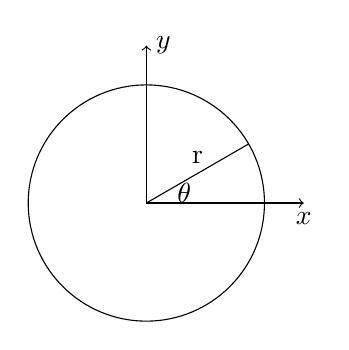
\begin{tikzpicture}
			\def\k{2};
			\node (O) at (0, 0) {};
			\node (A) at (0,1.5) {};
			\node (B) at (30:1.5) {} ;	
			\draw [ ->] (0,0) --  (\k,0)  node[below] {$x$};
			\draw [ ->]  (0,0) -- ( 0,\k)   node[right] {$y$};
			\draw  (0,0) -- (30:1.5) node[midway,above] {r};
			\draw (0,0) circle (1.5cm);
			\path (0,0) ++(15: .5) node{$\theta$};
		\end{tikzpicture}
	\end{center}
\end{frame}	

\begin{frame}
	\alert{ 解:}	这是一个温度场,是非稳恒场,服从热传导方程:\\
	$\begin{cases}
		u_t=a^2 [u_{xx}   +u_{yy}] ~~~~ (0< x^2 +y^2 <r_0 ^2, t>0)\\
		u(x,y,t)|_{x^2+y^2=r_0 ^2}= 0 \\
		u(x,y,t)|_{t=0}= \Psi(x,y)
	\end{cases} $\\	\vspace{0.6em}
	考虑到圆域边界条件,得使用极坐标描述\\
\end{frame}

\begin{frame}
	\frametitle{}
	试证明极坐标拉普拉斯算子为:
	\[[u_{xx}   +u_{yy}]= [ {	\frac{\partial^2 u }{\partial r^2 } +\frac{1}{r } \frac{\partial u }{\partial r } +
	\frac{1}{r^2 } \frac{\partial ^2 u }{\partial \theta ^2
	} }]\]
	\证 ~基本变换关系为 
\[ \begin{cases}
	 x=r\cos \theta\\
	 y=r\sin \theta
	\end{cases}\]
对于函数 $ u(x,y)=u(r\cos \theta,r\sin \theta)$ 计算导数:
\[
\begin{aligned}
	\frac{\partial u}{\partial r}&=\frac{\partial u}{\partial x } \frac{\partial x}{\partial r }+  \frac{\partial u}{\partial y } \frac{\partial y}{\partial r } = \cos \theta \frac{\partial u}{\partial x } +  \sin \theta \frac{\partial u}{\partial y } \\
	\frac{\partial u}{\partial \theta}&=\frac{\partial u}{\partial x } \frac{\partial u}{\partial \theta }+  \frac{\partial u}{\partial y } \frac{\partial y}{\partial \theta } = -r \sin \theta \frac{\partial u}{\partial x } +  r\cos \theta \frac{\partial u}{\partial y } \\
\end{aligned}\]
\end{frame}

\begin{frame}
	改写成矩阵形式:
	\[ 
\begin{aligned}
	&\begin{bmatrix}
	   \frac{\partial u}{\partial r} \\
	   \frac{\partial u}{\partial \theta} 
	\end{bmatrix}
	=
	\begin{bmatrix}
		\cos \theta &  \sin \theta \\
		-r \sin \theta& r\cos \theta \\  
	\end{bmatrix}
	\begin{bmatrix}
		\frac{\partial u}{\partial x} \\
		\frac{\partial u}{\partial y} 
	 \end{bmatrix}\\
	&\begin{bmatrix}
		\frac{\partial u}{\partial r} \\
		\frac{\partial u}{\partial \theta} 
	 \end{bmatrix}
	 =
	 \begin{bmatrix}
		1 &  0 \\
		0 & r \\  
	\end{bmatrix}
	 \begin{bmatrix}
		 \cos \theta &  \sin \theta \\
		 -\sin \theta& \cos \theta \\  
	 \end{bmatrix}
	 \begin{bmatrix}
		 \frac{\partial u}{\partial x} \\
		 \frac{\partial u}{\partial y} 
	  \end{bmatrix}\\
	 &\begin{bmatrix}
		\frac{\partial u}{\partial x} \\
		\frac{\partial u}{\partial y} 
	 \end{bmatrix}
	 =
	 \begin{bmatrix}
		 \cos \theta &  -\sin \theta \\
		 \sin \theta& \cos \theta \\  
	 \end{bmatrix}
	 \begin{bmatrix}
		1 &  0 \\
		0 & 1/r \\  
	\end{bmatrix}
	 \begin{bmatrix}
		 \frac{\partial u}{\partial r} \\
		 \frac{\partial u}{\partial \theta} 
	  \end{bmatrix}\\
\end{aligned}
	  \]
\end{frame}


\begin{frame}
	\frametitle{}
	\[ 
\begin{aligned}
	 &\begin{bmatrix}
		\frac{\partial u}{\partial x} \\
		\frac{\partial u}{\partial y} 
	 \end{bmatrix}
	 =
	 \begin{bmatrix}
		 \cos \theta &  -\sin \theta \\
		 \sin \theta& \cos \theta \\  
	 \end{bmatrix}
	 \begin{bmatrix}
		 \frac{\partial u}{\partial r} \\
		\frac{1}{r} \frac{\partial u}{\partial \theta} 
	  \end{bmatrix}\\
	&\begin{bmatrix}
		\frac{\partial u}{\partial x} \\
		\frac{\partial u}{\partial y} 
	 \end{bmatrix}
	 =
	 \begin{bmatrix}
		 \vec{e}_r & \vec{e}_\theta 
	 \end{bmatrix}
	 \begin{bmatrix}
		 \frac{\partial u}{\partial r} \\
		\frac{1}{r} \frac{\partial u}{\partial \theta} 
	  \end{bmatrix} \\
	&\nabla= \vec{e}_r \frac{\partial }{\partial r} +   \vec{e}_\theta \frac{1}{r} \frac{\partial }{\partial \theta} \\
	&\begin{aligned}
		\nabla ^2 &=\nabla \cdot \nabla \\
		&= (\vec{e}_r \frac{\partial }{\partial r} +   \vec{e}_\theta  \frac{1}{r}\frac{\partial }{\partial \theta})\cdot (\vec{e}_r \frac{\partial }{\partial r} +   \vec{e}_\theta \frac{1}{r} \frac{\partial }{\partial \theta})\\
	\end{aligned}	
\end{aligned}	
	\] 
\end{frame}

\begin{frame}
	\[ \begin{aligned}
	\nabla ^2 &= \vec{e}_r \cdot\frac{\partial }{\partial r}  (\vec{e}_r \frac{\partial }{\partial r} +   \vec{e}_\theta \frac{1}{r} \frac{\partial }{\partial \theta})+  \vec{e}_\theta \cdot \frac{1}{r} \frac{\partial }{\partial \theta} (\vec{e}_r \frac{\partial }{\partial r} +   \vec{e}_\theta \frac{1}{r} \frac{\partial }{\partial \theta})\\
	&=\vec{e}_r \cdot (\frac{\partial \vec{e}_r}{\partial r} \frac{\partial }{\partial r} + \vec{e}_r \frac{\partial ^2 }{\partial r ^2}+  \frac{\partial \vec{e}_\theta}{\partial r} \frac{1}{r}\frac{\partial }{\partial \theta}+  \vec{e}_\theta\frac{\partial }{\partial r} (\frac{1}{r}\frac{\partial }{\partial \theta})) \\
	&\hspace{1em} + \vec{e}_\theta \cdot (\frac{1}{r}\frac{\partial \vec{e}_r}{\partial \theta} \frac{\partial }{\partial r} + \vec{e}_r \frac{1}{r} \frac{\partial }{\partial \theta} \frac{\partial }{\partial r} + \frac{1}{r} \frac{\partial  \vec{e}_\theta}{\partial \theta} \frac{1}{r} \frac{\partial }{\partial \theta} + \vec{e}_\theta \frac{1}{r} \frac{\partial }{\partial \theta} (\frac{1}{r} \frac{\partial }{\partial \theta} )
	) \\
	&=\vec{e}_r \cdot (0 \frac{\partial }{\partial r} + \vec{e}_r \frac{\partial ^2 }{\partial r ^2}+  0\frac{\partial }{\partial \theta}+  \vec{e}_\theta\frac{\partial }{\partial r} (\frac{1}{r}\frac{\partial }{\partial \theta})) \\
	&\hspace{1em} + \vec{e}_\theta \cdot (\vec{e}_\theta \frac{1}{r}\frac{\partial }{\partial r} + \vec{e}_r \frac{1}{r} \frac{\partial }{\partial \theta} \frac{\partial }{\partial r} + \frac{1}{r} (-\vec{e}_r) \frac{1}{r} \frac{\partial }{\partial \theta} + \vec{e}_\theta \frac{1}{r^2} \frac{\partial ^2 }{\partial \theta ^2}
	) \\
	&=  \frac{\partial^2  }{\partial r^2 } +\frac{1}{r } \frac{\partial  }{\partial r } +\frac{1}{r^2 } \frac{\partial ^2  }{\partial \theta ^2} 
	\end{aligned}\] 
~\\ \vspace{1em}
\alert{\textit{Tips:\hspace{1em}}} $\frac{\partial  \vec{e}_\theta}{\partial \theta}=-\vec{e}_r ;\quad \frac{\partial  \vec{e}_\theta}{\partial r}=0 ;  \quad \frac{\partial  \vec{e}_r}{\partial r}=0 ; \quad\frac{\partial  \vec{e}_r}{\partial \theta}=\vec{e}_\theta $ 
\end{frame}

\begin{frame}
	\frametitle{极坐标系下的方程}
	$\begin{cases}
		\displaystyle	u_t=a^2 [ {	\frac{\partial^2 u }{\partial r^2 } +\frac{1}{r } \frac{\partial u }{\partial r } +
		\frac{1}{r^2 } \frac{\partial ^2 u }{\partial \theta ^2
		} }], ~~~~ (0<r<r_0, t>0)\\
		u(r_0,\theta)=0,~~~~~~~~~~~~ 0<\theta <2\pi 	\\
		u(r,\theta,t =0)=\Psi(r,\theta) ,~~~~~~~~~~~~ 0<\theta <2\pi 	
	\end{cases} $\\
	令:$u(r,\theta,t) =R(r)\Theta(\theta)T(t)$,  代回原方程,得:
	\begin{equation*}
		R\Theta T'=a^2 [ R'' \Theta T + \dfrac{1}{r} R' \Theta T  + \dfrac{1}{r^2} R \Theta '' T(t)  ]
	\end{equation*}
	整理:
	\begin{equation*}
		\frac{T'}{a^2T} =\frac{R''}{R}+\frac{1}{r} \frac{R'}{R} +\frac{1}{r^2} \frac{\Theta ''} {\Theta}  =-\lambda
	\end{equation*}
	转化为两个方程:
	\begin{equation*}
		T'(t)+\lambda a^2T(t)=0  ~~~~~....... ~~~~~~(1)
	\end{equation*}	
	方程1是衰减模型,已求解!\\
\end{frame}	

\begin{frame}
	\begin{equation*}
		r^2 \frac{R'' (r)}{R(r)}+r \frac{R'(r)}{R(r)} + \lambda r^2 +\frac{\Theta ''(\theta)} {\Theta (\theta)} =0  ~~~~~~......~~(2)
	\end{equation*}
	方程2是固有值问题,可继续分离变量:	
	\begin{equation*}
		r^2 \frac{R'' (r)}{R(r)}+r \frac{R'(r)}{R(r)} + \lambda r^2 =-\frac{\Theta ''(\theta)} {\Theta (\theta)} =\mu  
	\end{equation*}
	角向固有值问题:
	$ \begin{cases}
		\Theta ''(\theta)+\mu \Theta (\theta) =0 \\
		\Theta (\theta) =	\Theta (\theta+2\pi)  \\
		\Theta' (\theta) =	\Theta' (\theta+2\pi)  
	\end{cases} $\\	
	径向固有值问题:
	$ \begin{cases}
		r^2 R'' (r)+r R'(r) +( \lambda r^2 -\mu)R(r)=0  \\
		R(r_0)=0
	\end{cases} $\\	
\end{frame}	

\begin{frame}
	角向固有值问题有解,\\
	固有值:
	\begin{equation*}
		\mu=n^2, ~~~~~(n=0,1,2,3...)
	\end{equation*}
	固有函数:
	\begin{equation*}
		\Theta_n(\theta) = a_n \cos(n\theta)+b_n \sin(n\theta), ~~~~~(n=0,1,2,3...)
	\end{equation*}
	\begin{equation*}
		\Theta_n(\theta) = \frac{1}{\sqrt{2\pi}} e^{-i n \theta }, ~~~~~(n=0,1,2,3...)
	\end{equation*}
	~\\
	把$\mu=n^2$,代回径向方程,得径向固有值问题:\vspace{0.6em}
	\[ \boxed{ \begin{cases}
		r^2 R'' (r)+r R'(r) +( \lambda r^2 -n^2)R(r)=0  \\
		R(r_0)=0
	\end{cases} }\]	
	称为贝塞尔方程	
\end{frame}	

\begin{frame}
	\begin{exampleblock} {例2、试证明圆域波动方程的径向固有值问题也是贝塞尔方程:}~ ~
	\end{exampleblock}
	\证~圆域波动方程如下:\\
	$\begin{cases}
		u_{tt}=a^2 [u_{xx}   +u_{yy}] ~~~~ (0< x^2 +y^2 <r_0 ^2, t>0)\\
		u(x,y,t)|_{x^2+y^2=r_0 ^2}= 0 \\
		u(x,y,t)|_{t=0}= \Psi(x,y) \\
		u_t (x,y,t)|_{t=0}= \varphi  (x,y) 
	\end{cases} $\\	\vspace{0.6em}
	考察方程,发现当使用极坐标拉普拉斯算子后,整个的分离变量过得与热传导方程高度一致,(*P115)\\
	其固有值问题也是贝塞尔方程!\\ \vspace{0.6em}
	$\begin{cases}
		r^2 R'' (r)+r R'(r) +( \lambda r^2 -n^2)R(r)=0  \\
		R(r_0)=0
	\end{cases} $\\		
\end{frame}	

\begin{frame}
	\frametitle{结论: }
	贝塞尔方程是圆域极坐标条件下的一个普适的径向本征方程! \\ \vspace{2em}
	\[\begin{cases}
		r^2 R'' (r)+r R'(r) +( \lambda r^2 -n^2)R(r)=0  \\
		R(r_0)=0
	\end{cases}  \]\\	
\end{frame}	

\begin{frame}	
	在正式求解之前,先预处理一下\\
	令:
	\begin{equation*}
		x=\sqrt{\lambda} r, ~~~~y(x)= R(r) =R(\frac{x}{\sqrt{\lambda}})
	\end{equation*}
	有: 
	\[
	\begin{aligned}
		&\frac{dy}{dx} = \frac{dR}{dr} \frac{dr}{dx} = \frac{1}{ \sqrt{\lambda}} \frac{dR}{dr}\\
		&\frac{d^2y}{dx^2} = \frac{1}{\lambda} \frac{dR^2}{dr^2}\\
	\end{aligned}	
	\]
	代回原方程,
\end{frame}	

\begin{frame}
	得:
	\begin{equation*}
		\boxed{x^2\frac{d^2y}{dx^2} + x\frac{dy}{dx} +(x^2 -n^2)y=0}
	\end{equation*}
	称为n整数阶贝塞尔方程.\\ \vspace{1em}
	{\Bullet}与欧拉方程比较:
	\begin{equation*}
		x^2\frac{d^2y}{dx^2} + x\frac{dy}{dx} +n^2y=0
	\end{equation*}
	欧拉方程是一个变系数微分方程,可通过变量代换(令$t=\ln x $) 转化为常系数微分方程
	\[ \frac{d^2y}{dt^2} - n^2y=0 \]
\end{frame}	

\begin{frame}
	若同样令$t=\ln x $, 贝塞尔方程转化为 
	\[ \frac{d^2y}{dt^2} +(x^2-n^2)y=0 \]
	依然是变系数微分方程,无法进一步进行求解.\\
	因此,贝塞尔方程没有通常意义的初等函数表达式解!
\end{frame}	

\begin{frame}
	\frametitle{方程的求解}
	\begin{exampleblock} {例2、求解贝塞尔方程}
		\begin{equation*}
			x^2\frac{d^2y}{dx^2} + x\frac{dy}{dx} +( x^2 -n^2)y=0
		\end{equation*}	
	\end{exampleblock}
	\alert{ 解:}~没有通常意义的初等函数表达式解,即没有通常意义的级数解,\\
	尝试,设方程有如下非一般意义的级数解:
	\begin{equation*}
		y=\sum\limits_{k=0}^{\infty} a_k x^{s+k},  \qquad (a_0 \not =0)
	\end{equation*}	
\end{frame}	

\begin{frame}
	求导:
	\begin{equation*}
		y'=\sum\limits_{k=0}^{\infty} (s+k) a_k x^{s+k-1}
	\end{equation*}	
	\begin{equation*}
		y''=\sum\limits_{k=0}^{\infty} (s+k) (s+k-1) a_k x^{s+k-2}
	\end{equation*}	
	代回原方程(注意脚标的变化),得:
	\begin{equation*}
		\sum\limits_{k=0}^{\infty} [(s+k) ^2 -n^2]  a_k x^{s+k} + \sum\limits_{k=2}^{\infty}  a_{k-2} x^{s+k} =0
	\end{equation*}	
	第一项(k=0)系数应为零:
	\begin{equation*}
		(s+k) ^2 -n^2=0,~~ \to s_1=-n, \qquad s_2=n. 
	\end{equation*}	
\end{frame}	

\begin{frame}
	第二项(k=1)系数应为零:
	\begin{equation*}
		[(s+k) ^2 -n^2] a_1=0,\qquad \to a_1=0. 
	\end{equation*}	
	后面各项系数都为零:
	\begin{equation*}
		[(s+k) ^2 -n^2] a_k+ a_{k-2}=0, ~~~ (k=2,3,4,...)
	\end{equation*}	
	存在递推关系:
	\begin{equation*}
		a_k=-\frac{1}{(s+k) ^2 -n^2 } a_{k-2}
	\end{equation*}	
	由$a_1=0$,可推出奇数项为零 \[a_{2m+1}=0\]
	现取$s=n$, (-n 不影响解题过程),得:
	\begin{equation*}
		a_{2m}=\frac{-1}{(n+2m) ^2 -n^2 } a_{2m-2} =\frac{-1}{2m (2n+2m) } a_{2m-2}, \qquad (m=1,2,3,...)
	\end{equation*}	
\end{frame}	

\begin{frame}
	归纳,得:
	\begin{equation*}
		a_{2m}=(-1)^m  \frac{1}{2^{2m} m! (n+m) (n+m-1)... (n+1) } a_0 
	\end{equation*}	
	取:$a_0=1/2^n n!$, 得:
	\begin{equation*}
		a_{2m}=(-1)^m  \frac{1}{2^{2m+n} m! (n+m) ! }
	\end{equation*}	
	贝塞尔方程有级数特解:
	\begin{equation*}
		y(x) = \sum\limits_{m=0}^{\infty} a_{2m} x^{n+2m} 
	\end{equation*}	
	分析收敛性,发现:
	\begin{equation*}
		\lim\limits_{m\to \infty}|\frac{ a_{2m+2}} {a_{2m}}|= \lim\limits_{m\to \infty}\frac{ 1}{4(m+1)(n+m+1)} =0
	\end{equation*}	
	说明此级数必为某函数的展开式,称之为贝塞尔函数。
\end{frame}	

\begin{frame}
	记为: \[\boxed{J_n(x) = \sum\limits_{m=0}^{\infty} a_{2m} x^{n+2m}} 
		 \]
	称为n整数阶贝塞尔函数! 
\end{frame}	

\begin{frame}
	\centering
	\includegraphics[width=0.8\textwidth]{bessel.png}
\end{frame}	

\begin{frame}
	\begin{center}
		\begin{figure}
			\includegraphics[width=4.2cm]{figs/fig1-3-6.png}	
		\end{figure}
	\end{center}
	贝塞尔(Bessel,Friedrich Wilhelm,1784~1846)德国天文学家,数学家,天体测量学的奠基人.
	提出贝塞尔函数,讨论该函数的一系列性质及其求值方法,为解决物理学、天文学和信息学有关问题提供了重要工具。
\end{frame}

\begin{frame}
	\frametitle{作业}
	1、由圆域波动方程导出贝塞尔方程\\
	2、求衰减模型
	\begin{equation*}
		T'(t)+\lambda a^2T(t)=0  
	\end{equation*}
	3、求角向固有值及归一化的固有函数:\\
	\[ \begin{cases}
		\Theta ''(\theta)+\mu \Theta (\theta) =0 \\
		\Theta (\theta) =	\Theta (\theta+2\pi)  \\
		\Theta' (\theta) =	\Theta' (\theta+2\pi)  
	\end{cases}  \]	
	4、求欧拉方程
\end{frame}	

\section{2.贝塞尔函数与Gamma函数}

\begin{frame}
	\frametitle{贝塞尔函数}
	零阶贝塞尔函数:
	\begin{equation*}
		J_0(x) = \sum\limits_{m=0}^{\infty} (-1)^m  \frac{1}{m! m! } (\frac{x}{2})^{2m} 
	\end{equation*}	
	n阶贝塞尔函数:
	\begin{equation*}
		J_n(x) = \sum\limits_{m=0}^{\infty} (-1)^m  \frac{1}{m! (n+m) ! } (\frac{x}{2})^{n+2m} 
	\end{equation*}	
	第二类贝塞尔函数:
	\begin{equation*}
		Y_{\alpha}(x)=\frac{J_{\alpha}(x) \cos (\alpha \pi)-J_{-\alpha}(x)}{\sin (\alpha \pi)}
	\end{equation*}	
	贝塞尔函数在除$x=0$点外的整个实数轴上收敛。
\end{frame}	

\begin{frame}
	\frametitle{$\Gamma$函数}
	为进一步讨论贝塞尔函数的性质,先讨论Gamma函数.\\  
	\begin{enumerate}
		\Item 1728年,哥德巴赫在考虑数列插值的问题, 比如我们可以计算2!,3!,是否可以计算2.5!呢? 
		\Item 他写信请教尼古拉斯·伯努利和他的弟弟丹尼尔·伯努利, 欧拉当时正好与丹尼尔·伯努利在一块,他因此得知了这个问题
		\Item 1729 年欧拉解决了这个问题! 
	\end{enumerate}
	\begin{figure}
		\centering
		\subfigure[]{\includegraphics[width=0.45\textwidth]{figs/2022-04-02-08-43-23.png}}
	\end{figure} 
	\setcounter{subfigure}{0}
\end{frame}	

\begin{frame}
	\frametitle{$\Gamma$函数的定义}	
	\begin{equation*}
		\Gamma(x)=\int_{0}^{\infty} t^{x-1} e^{-t} dt, \qquad (x>0)
	\end{equation*}	
	
	Euler创造的$\Gamma$函数,将积分和阶乘联系在起来\\ \vspace{0.6em}
	\例 [1.试证明]
	{ \[
		\Gamma(1)=1
	   \]}
	\证 ~	
\[ \begin{aligned}
	\Gamma(1)&=\int_{0}^{\infty} t^{1-1} e^{-t} dt \\	
			&=\int_{0}^{\infty}  e^{-t} dt =1	
\end{aligned}\]
\end{frame}	

\begin{frame}	
	\frametitle{~$\Gamma$函数的性质}
	\alert{性质1:} ~试证明Gamma函数有如下递推式:
		\[\Gamma(x+1)=x \Gamma(x),\qquad (x>0)\]
	\alert{证明:}  
	\begin{equation*}
	\begin{split}
		\Gamma(x+1)&= \int_{0}^{\infty} t^{x+1-1} e^{-t} dt \\
		&= -t^x e^{-t} |_0 ^\infty + x \int_{0}^{\infty} t^{x-1} e^{-t} dt \\
		&= x \int_{0}^{\infty} t^{x-1} e^{-t} dt \\
		&=x \Gamma(x)
	\end{split}
	\end{equation*}	
\end{frame}	

\begin{frame}
	 推论: 
	\begin{equation*}
		\Gamma(x+n)=(x+n-1)(x+n-2)\cdots (x+1)x\Gamma(x)
	\end{equation*}	 
\end{frame}	

\begin{frame}
	\alert{性质2:}~试证明自变量为正整数的Gamma函数与阶乘有如下关系:
	\begin{equation*}
		\Gamma(n+1)=n!
	\end{equation*}	
	\alert{证明1:}  由递推公式
	\begin{equation*}
	\begin{split}
		\Gamma(x+1)&=x \Gamma(x) \\
		\Gamma(n+1)&=n \Gamma(n) \\
		&=n(n-1)\cdots 1 \Gamma(1) \\
		&=n! \int_{0}^{\infty}  e^{-t} dt \\
		&=n!
	\end{split}
	\end{equation*}	
\end{frame}	

\begin{frame}
	\alert{证明2:}  	 在推论中:取$x=1$
	\begin{equation*}
	\begin{split}	
		\Gamma(x+n)&=(x+n-1)(x+n-2)\cdots (x+1)x\Gamma(x)\\
		\Gamma(1+n)&=(1+n-1)(1+n-2)\cdots (1+1)1\Gamma(1)\\
		\Gamma(n+1)&=n!
	\end{split}
	\end{equation*}	 
	~~\\ \vspace{4em}
\alert{\textit{Tips:\hspace{1em}}} ~ 阶乘只是$\Gamma(x)$函数的特例!$(x=1,2,3,\cdots)$对应$ (0!, 1!, 2!,\cdots)$
\end{frame}	


\begin{frame}
	\alert{性质3:} 试证明半正整数$\Gamma$函数有如下性质 
	\begin{equation*}
		\begin{split}
		\Gamma(\frac{1}{2}) &=\sqrt{\pi} \\ 
		\qquad  \Gamma(n+\frac{1}{2}) &= \frac{(2n-1)!!}{2^n} \sqrt{\pi}
		\end{split}	
	\end{equation*}	
	\alert{证明:}  (1) 由Gamma函数定义
	\[
	\begin{aligned}
		 \Gamma(x)&=\int_{0}^{\infty} t^{x-1} e^{-t} dt, \qquad (x>0) \\
		 \Gamma(\frac{1}{2})&=\int_{0}^{\infty} t^{\frac{1}{2}-1} e^{-t} dt\\
		 &=\int_{0}^{\infty} \frac{1}{\sqrt{t}} e^{-t} dt\\
	\end{aligned}	
	\]
\end{frame}

\begin{frame}
	  \frametitle{}
	  令$x=\sqrt{t}$
	  \[
		\begin{aligned}
			 \Gamma(\frac{1}{2})
			 &=2\int_{0}^{\infty} e^{-x^2} dx\\
			 &=2\sqrt{\iint_{0}^{\infty} e^{-x^2} e^{-y^2} dxdy}\\
			 &=2\sqrt{\int_{0}^{\frac{\pi}{2}} \int_{0}^{\infty}  e^{-r^2} r dr d\theta}\\
			 &=2\sqrt{\frac{\pi}{2} \int_{0}^{\infty} r e^{-r^2} dr }\\
			 &=2\sqrt{\frac{\pi}{2}[-\frac{1}{2} e^{-r^2}]_{0}^{\infty} }\\
			 &=\sqrt{\pi}
		\end{aligned}	
		\]  
	* x,y皆取正数,是第一象限!			
\end{frame}	

\begin{frame}
	  \frametitle{}
	  (2) 由递推公式 $\Gamma(1+x)=x \Gamma(x) ,\qquad (x>0)$\\
	  \[
	\begin{aligned}
		\Gamma(1+\frac{1}{2})&= \frac{1}{2} \Gamma(\frac{1}{2}) =\frac{1}{2} \sqrt{\pi}\\
		\Gamma(2+\frac{1}{2})&= \Gamma(1+\frac{3}{2})=\frac{3}{2} \Gamma(1+\frac{1}{2}) = \frac{3}{2}\frac{1}{2}\sqrt{\pi}\\
		\Gamma(3+\frac{1}{2})& = \frac{5}{2} \frac{3}{2}\frac{1}{2}\sqrt{\pi}\\
		\Gamma(n+\frac{1}{2})& = \frac{(2n-1)!!}{2^n}\sqrt{\pi}\\
		 & = \frac{(2n)!}{2^{2n} n!}\sqrt{\pi}
	\end{aligned} 
	  \]
	证毕!
\end{frame}

\begin{frame}
	\alert{性质4:} 试证明半正整数的阶乘为
	\[(\frac{1}{2})! =  \frac{\sqrt{\pi}}{2}\]
	\[ (m-\frac{1}{2})! =\frac{(2m)!}{2^{2m} m!}\sqrt{\pi} \]
	\alert{证明:} 把如下公式从正整数向正实数延拓!
	\[\Gamma(n+1)=n!\qquad \to \qquad \Gamma(x+1)=x!, (x>0)\]
	(1) 取:$x=m-\frac{1}{2}, \qquad (m=1,2,3, \cdots )$
	\[ \begin{aligned}
		(m-\frac{1}{2})! &= \Gamma (m-\frac{1}{2}+1) \\
						 &= \Gamma (m+\frac{1}{2}) \\
						 & = \frac{(2m)!}{2^{2m} m!}\sqrt{\pi} 
	\end{aligned} \]
\end{frame}

\begin{frame}
	(2) 在上式中取$m=1$
	\[(\frac{1}{2})! =  \frac{\sqrt{\pi}}{2} \]
	~~ \\ \vspace{1em}
* 一般分数的阶乘如何求?(余元公式,Gamma函数定义式)
\[ \Gamma(x)  \Gamma(1-x) =\frac{\pi}{\sin x \pi}, \qquad  0<x<1 \]
\[ \Gamma(\frac{1}{2}+x)  \Gamma(\frac{1}{2}-x) =\frac{\pi}{\cos x \pi}, \qquad  0<x<\frac{1}{2} \]
 * 例如,求$(\pi) !$ 
 \[ (\pi)! = \Gamma(\pi +1 ) = \int_{0}^{\infty} t^{\pi} e^{-t} dt =? \]
\end{frame}

\begin{frame}
	\alert{性质5:} 试求半负整数$\Gamma$函数的值
	\begin{equation*}
		\begin{split}
		\Gamma(-\frac{1}{2}) &=-2\sqrt{\pi} \\ 
		\Gamma(-\frac{3}{2}) &=\frac{4}{3}\sqrt{\pi}
		\end{split}	
	\end{equation*}	
	\alert{解:} (1) 把递推公式 $\Gamma(1+x)=x \Gamma(x)$ 从正实数向实数延拓! \\
	并令$x=-\dfrac{1}{2}$\\
	\[
	\begin{aligned}
		 \Gamma(-\frac{1}{2})&= -2 \Gamma(1-\frac{1}{2})\\
		 &=-2 \Gamma(\frac{1}{2})\\
		 &=-2 \sqrt{\pi}
	\end{aligned}	
	\]
\end{frame}

\begin{frame}
	  \frametitle{}
	(2) 在递推公式 $\Gamma(1+x)=x \Gamma(x)$中, 令$x=-\dfrac{3}{2}$\\
	\[
	\begin{aligned}
		 \Gamma(-\frac{3}{2})&= -\frac{2}{3} \Gamma(1-\frac{3}{2})\\
		 &=-\frac{2}{3} \Gamma(-\frac{1}{2})\\
		 &=(-\frac{2}{3})(-2 \sqrt{\pi}) \\
		 &=\frac{4}{3}\sqrt{\pi} \\
	\end{aligned}	
	\] 
\end{frame}

\begin{frame}
	* 从正实数$x>0$向实数延拓 $x \in \mathbb{R} $, 导致严重的问题, 比如: 
	\[ n! =(n-1)(n-2)(n-3)\cdots 1\]
	\[ (-1)! =(-1)(-2)(-3)\cdots -\infty ? \] 
	\[\Gamma(0)= (-1)! \quad ? , \qquad \Gamma(-1)=?, \cdots\] 
	\alert{性质6:} ~试证明Gamma函数在非正整数点的极限为无穷大
	\begin{equation*}
		\lim\limits_{x\to -n }\Gamma(x)=\infty, \qquad (n=0,1,2, \cdots)
	\end{equation*}	
		\[ \frac{1}{\Gamma(-n)} =0, \qquad (n=0,1,2, \cdots) \]
\end{frame}		
\begin{frame}
\alert{证明:}  由递推公式
	\begin{equation*}
	\begin{split}
		\Gamma(x)&=\frac{1}{x} \Gamma(x+1) \\
		\lim\limits_{x\to 0 }	\Gamma(x)&=	\lim\limits_{x\to 0 } \frac{1}{x} \Gamma(x+1) =\infty \\
		\lim\limits_{x\to -1 }	\Gamma(x)&=\lim\limits_{x\to -1 } \frac{1}{x} \Gamma(x+1) =  \lim\limits_{x\to 0 } \frac{1}{x-1} \Gamma(x) =\infty \\
		& \cdots \cdots	\\	
		\lim\limits_{x\to -n }	\Gamma(x)&=\lim\limits_{x\to -n } \frac{1}{x} \Gamma(x+1) = \lim\limits_{x\to -(n-1) } \frac{1}{x-1} \Gamma(x) =\infty  
	\end{split}
	\end{equation*}	
	证毕! \\ \vspace{1em}
\alert{\textit{Tips:\hspace{1em}}} \\ 
延拓到实数域后, $\Gamma$函数存在奇点$x = 0,-1,-2,\cdots$,如果进一步延拓到复数域, 这些奇点依然存在.它们是$\Gamma$函数的一阶极点!
\end{frame}	

\begin{frame}
	\frametitle{实数域Gamma函数}
  \begin{center}
	   \includegraphics[width=0.85\textwidth,height=2.9in]{figs/2022-04-03-09-17-41.png}
  \end{center}
\end{frame}

\begin{frame}
	\frametitle{复数域Gamma函数}
  \begin{center}
	   \includegraphics[width=0.85\textwidth,height=2.5in]{figs/2022-03-26-17-20-10.png}
  \end{center}
  网络教学资源, \href{https://www.bilibili.com/video/av892512155/}{点这里}
\end{frame}

\begin{frame}
	\frametitle{Gamma 函数的应用实例}
	\例 [1. 计算如下积分]{
	\[ (1)~\int_{0}^{\infty} x^2 e^{-x^2} dx, \qquad (2)~\int_{0}^{\infty} x^2 e^{-\frac{1}{2}x^2} dx \]}
	\解 ~ 比较(1)式与Gamma函数的定义式的结构,
	\[\Gamma(x)=\int_{0}^{\infty} t^{x-1} e^{-t} dt, \qquad (x>0)\]
	\[\begin{aligned}
		\int_{0}^{\infty} x^2 e^{-x^2} dx &= \int_{0}^{\infty} (x^2)^1 e^{-(x^2)} \frac{1}{2x}d(x^2)\\
		&= \frac{1}{2}\int_{0}^{\infty} (x^2)^{\frac{1}{2}} e^{-(x^2)} d(x^2)\\	
		&= \frac{1}{2}\int_{0}^{\infty} t^{\frac{1}{2}} e^{-t} d(t)
	\end{aligned} \]
\end{frame}

\begin{frame}
	  \frametitle{}
	  \[\begin{aligned}
		\int_{0}^{\infty} x^2 e^{-x^2} dx &= \frac{1}{2}\int_{0}^{\infty} t^{\frac{3}{2}-1} e^{-t} d(t)\\	
		&= \frac{1}{2}\Gamma(\frac{3}{2})  \\ 
		&= \frac{1}{2}\Gamma(1+\frac{1}{2})  \\ 
		&= \frac{1}{2} \frac{1}{2} \Gamma(\frac{1}{2})  \\ 
		&= \frac{\sqrt{\pi}}{4} 
	\end{aligned} \]
\end{frame}

%%%%%%%%%%%%%%%%%%%%%%%%%%%%%%%%%%%%%%%%%%%%%%%%%%%%%%%%%%%%%%%%%%%
\begin{frame}
	\frametitle{课外作业}
	\begin{enumerate}
		\item 求 $0!, \qquad \int_{0}^{\infty} x^2 e^{-\frac{1}{2}x^2} dx $
		\item 试证明 $ \frac{1}{\Gamma(-n)} =0, \qquad (n=0,1,2, \cdots) $
		\item 试证明半正整数$\Gamma$函数值的一般性公式
		\[ (m-\frac{1}{2})! =\frac{(2m)!}{2^{2m} m!}\sqrt{\pi} \qquad (m=1,2,3,\cdots) \]
		\item 试求出半负整数$\Gamma$函数值的一般性公式
		\[\Gamma(m-\frac{1}{2})=?, \qquad (m=0,-1,-2,-3,\cdots)\]	
	\end{enumerate}
\end{frame}
%%%%%%%%%%%%%%%%%%%%%%%%%%%%%%%%%%%%%%%%%%%%%%%%%%%%%%%%%%%%%%%%%%%

\section{3.贝塞尔函数的性质}

\begin{frame}
	现在讨论贝塞尔函数的性质:\\
	\alert{性质1:} 负数阶贝塞尔函数与正数阶贝塞尔函数有如下关系
	\begin{equation*}
		J_{-n}(x)=(-1)^n J_n(x)
	\end{equation*}	
	\alert{证明:}  
	用$\Gamma$ 函数重写出贝塞尔函数:
	\begin{equation*}
		J_n(x) = \sum\limits_{m=0}^{\infty} (-1)^m  \frac{1}{m! (n+m) ! } (\frac{x}{2})^{n+2m} 
	\end{equation*}	
	\begin{equation*}
		J_n(x) = \sum\limits_{m=0}^{\infty} (-1)^m  \frac{1}{m! \Gamma(n+m+1) } (\frac{x}{2})^{n+2m} 
	\end{equation*}	
	负数阶塞尔函数可写成
	\begin{equation*}
		J_{(-n)}(x) = \sum\limits_{m=0}^{\infty} (-1)^m  \frac{1}{m! \Gamma(-n+m+1) } (\frac{x}{2})^{-n+2m} 
	\end{equation*}	
\end{frame}	

\begin{frame}
	对于 $m<n$ 的项,分母中的Gamma函数为无穷大,因此都为零,要去除:
	\begin{equation*}
		J_{(-n)}(x) = \sum\limits_{m=n}^{\infty} (-1)^m  \frac{1}{m! \Gamma(-n+m+1) } (\frac{x}{2})^{-n+2m} 
	\end{equation*}	
	令 $m-n=k$, 有 $m=n+k $, 
	\begin{equation*}
		J_{(-n)}(x) = (-1)^n\sum\limits_{k=0}^{\infty} (-1)^k  \frac{1}{(n+k)! \Gamma(k+1) } (\frac{x}{2})^{n+2k} 
	\end{equation*}	
	\begin{equation*}
		J_{-n} (x) = (-1)^n\sum\limits_{k=0}^{\infty} (-1)^k  \frac{1}{(n+k)! k! } (\frac{x}{2})^{n+2k} =(-1)^n J_{n} (x)
	\end{equation*}	
	证毕!
\end{frame}	

\begin{frame}
	\alert{性质2:} 半整数阶贝塞尔函数与三角函数有如下关系
	\begin{equation*}
		J_{1/2} (x) =\sqrt{\frac{2}{\pi x}} \sin x,  \qquad  J_{-1/2} (x) =\sqrt{\frac{2}{\pi x}} \cos x
	\end{equation*}	
	\alert{证明:}  基于Gamma函数,可以写出半整数阶贝塞尔函数
	\begin{equation*}
		J_n(x) = \sum\limits_{m=0}^{\infty} (-1)^m  \frac{1}{m! \Gamma(n+m+1) } (\frac{x}{2})^{n+2m} 
	\end{equation*}	
	\begin{equation*}
		J_{1/2}(x) = \sum\limits_{m=0}^{\infty} (-1)^m  \frac{1}{m! \Gamma(1/2+m+1) } (\frac{x}{2})^{1/2+2m} 
	\end{equation*}	
\end{frame}	

\begin{frame}
	其中, 
	\begin{equation*}
		\begin{split}
			\Gamma(1/2+m+1) &= (\frac{2m+1}{2}) \Gamma(1/2+m) \\
			& = (\frac{2m+1}{2}\frac{2m-1}{2})  \Gamma(1/2+m-1) \\
			&\cdots \cdots \\
			& = \frac{(2m+1)!!}{2^{m+1}} \Gamma(1/2) \\
			& = \frac{(2m+1)!!}{2^{m+1}} \sqrt{\pi} \\
		\end{split}	
	\end{equation*}	
\end{frame}	

\begin{frame}
	代回,有:
	\begin{equation*}
		J_{1/2}(x) = \sqrt{\frac{2}{\pi x}} \sum\limits_{m=0}^{\infty} (-1)^m  \frac{x^{2m+1}}{(2m+1)!} 
	\end{equation*}	 
	\begin{equation*}
		J_{1/2}(x) = \sqrt{\frac{2}{\pi x}} \sin x  
	\end{equation*}	 
	同理,有 
	\begin{equation*}
		J_{-1/2}(x) = \sqrt{\frac{2}{\pi x}} \cos x  
	\end{equation*}	 
	\alert{证毕!} 
\end{frame}

\begin{frame}
	\frametitle{课堂作业}
	\begin{enumerate}
		\item 求 \[\Gamma(-\frac{1}{2}), (-\frac{1}{2}) !\]
		\item 证明: \[ J_{-1/2}(x) = \sqrt{\frac{2}{\pi x}} \cos x \]
	\end{enumerate}
\end{frame}

\begin{frame}
	\alert{性质3:} 贝塞尔函数的导数与递推式 \\
	\begin{equation*}
		\begin{split}
			\frac{d}{d x}\left[x^{n} J_{n}(x)\right]= &x^{n} J_{n-1}(x),\qquad \cdots (1) \\
			\frac{d}{d x}\left[x^{-n} J_{n}(x)\right]=& -x^{-n} J_{n+1}(x) ,\qquad \cdots (2) \\
			2 n J_{n}(x)=&xJ_{n-1}(x)+x J_{n+1}(x) ,\qquad \cdots (3) \\
			2 J_{n}^{\prime}(x)=&J_{n-1}(x)-J_{n+1}(x) ,\qquad \cdots (4) 
		\end{split}
	\end{equation*}		
	由贝塞尔函数的$\Gamma$函数形式 
	\begin{equation*}
		J_n(x) = \sum\limits_{m=0}^{\infty} (-1)^m  \frac{1}{m! \Gamma(n+m+1) } (\frac{x}{2})^{n+2m} 
	\end{equation*}	 
	\alert{证明(1)式} : 上等式两端同乘$x^n$ 再求导:
	\begin{equation*}
	\begin{split}
		\frac{d}{dx} [x^n J_n(x)]&= \frac{d}{dx}\sum\limits_{m=0}^{\infty} (-1)^m  
		\frac{1}{m! \Gamma(n+m+1) } (\frac{x^{2n+2m}}{2^{n+2m}})\\	
	\end{split}
	\end{equation*}		
\end{frame}	

\begin{frame}
	\begin{equation*}
		\begin{split}
			\frac{d}{dx} [x^n J_n(x)] &=\sum\limits_{m=0}^{\infty} (-1)^m  
			\frac{1}{m! \Gamma(n+m+1) } (\frac{(2n+2m)x^{2n-1+2m}}{2^{n+2m}})\\
			&=x^n\sum\limits_{m=0}^{\infty} (-1)^m  
			\frac{1}{m! \Gamma(n-1+m+1) } (\frac{x^{n-1+2m}}{2^{n-1+2m}})\\ 
			&=x^n J_{n-1}(x) ,\qquad \cdots (1) 
		\end{split}
	\end{equation*}	
	\alert{证明 (2)式}: 同理,得:
	\begin{equation*}
		\begin{split}
		\frac{d}{d x}\left[x^{-n} J_{n}(x)\right]&=-x^{-n} J_{n+1}(x) ,\qquad \cdots (2) \\
		\end{split}
	\end{equation*}	 
\end{frame}

\begin{frame}
	\alert{证明 (3)和(4)式}: 把(1)(2)二式左端求导
	\begin{equation*}
		\begin{split}
			\frac{d}{dx} [x^n J_n(x)] &=n x^{n-1} J_n(x) + x^n J'_n(x)=x^n J_{n-1}(x) \\
			\frac{d}{d x}\left[x^{-n} J_{n}(x)\right]&=-n x^{-n-1} J_n(x) + x^{-n} J'_n(x)= -x^{-n} J_{n+1}(x)
		\end{split}
	\end{equation*}	
两式消去$J'_n(x)$得:
	\begin{equation*}
		2 n J_{n}(x)=x J_{n-1}(x)+x J_{n+1}(x)  ,\qquad \cdots (3)
	\end{equation*}	 	
两式消去$J_n(x)$得:
	\begin{equation*}
	2 J_{n}^{\prime}(x)=J_{n-1}(x)-J_{n+1}(x)  ,\qquad \cdots (4)
	\end{equation*}	 
\alert{证毕!} 
\end{frame}

\begin{frame}
	\alert{性质4:} 证明n阶贝塞尔函数有如下零点近似公式
	\[ \mu_{m}^{n} \approx m \pi+\frac{n \pi}{2}+\frac{3 \pi}{4}\]
	\alert{解:}对n(整数)阶贝塞尔方程
	\begin{equation*}
		x^2\frac{d^2y}{dx^2} + x\frac{dy}{dx} +(x^2 -n^2)y=0
	\end{equation*}
	做变量代换 \[ y=\frac{u}{\sqrt{x}}\] 
	得到 u(x)的方程:
	\begin{equation*}
		u'' +[1+\frac{\frac{1}{4}-n^2}{x^2}] u=0
	\end{equation*}
	当$x \to \infty $ 有方程:
	\begin{equation*}
		u'' + u=0 
	\end{equation*}	
\end{frame}	

\begin{frame}
	通解为:\[u=A\cos(x+\theta)\]
	确定A和$\theta$ (不证),得n阶贝塞尔函数的渐近公式\\
	\begin{equation*}
		J_{n}(x) \approx \sqrt{\frac{2}{\pi x}} \cos \left(x-\frac{n \pi}{2}-\frac{\pi}{4}\right)
	\end{equation*}
	令$J_{n}(x)=0$,由上式可得n阶贝塞尔函数的零点近似公式:
	\begin{equation*}
		\mu_{m}^{n} \approx m \pi+\frac{n \pi}{2}+\frac{3 \pi}{4}
	\end{equation*}
\end{frame}	


\begin{frame}
	\frametitle{固有值问题}
	对于圆域热传导方程或波动方程,其径向方程为
	\[\begin{cases}
		r^2 R'' (r)+r R'(r) +( \lambda r^2 -n^2)R(r)=0  \\
		R(r_0)=0
	\end{cases}  \]
	解为n阶贝塞尔函数$R(r)=J_n(x) = J_n(\sqrt{\lambda}r)$ \\ \vspace*{2em}
	{\Bullet} 零边界条件 $R(r_0)=0$对应$J_n(\sqrt{\lambda}r_0)=0$\\ 
	因此零边界条件下的本征解, 正是贝塞尔函数的零点!
\end{frame}	

\begin{frame}
	基此确定:\\	
	(1)固有值:
	\[ \sqrt{\lambda}r_0 = \mu_{m}^{n}  \qquad \to \qquad \lambda_m ^n =(\frac{\mu_{m}^{n}}{r_0})^2 \]
	(2)固有函数:\[R_m ^n(r) = J_n (\frac{\mu_{m}^{n}}{r_0}r) \]
\end{frame}

\begin{frame}
	\frametitle{}
	\alert{性质5:} 试证明n阶贝塞尔函数有如下零点递推式
	\[ J'_n(\mu_m ^n)= - J_{n+1}(\mu_m ^n)\]
	\alert{证明:}~由微分公式(2) 
 	\begin{equation*}
	\begin{split}
	 \frac{d}{d x}\left[x^{-n} J_{n}(x)\right]=& -x^{-n} J_{n+1}(x) ,\qquad \cdots (2) \\
	 -n x^{-n-1} J_n(x) + x^{-n} J'_n(x)&= -x^{-n} J_{n+1}(x) \\
	 -n J_n(x) + x J'_n(x)&= -x J_{n+1}(x) \\
	 -n 0 + x J'_n(\mu_m ^n)&= -x J_{n+1}(\mu_m ^n) \\
	 J'_n(\mu_m ^n)&= - J_{n+1}(\mu_m ^n)
 	\end{split}
	\end{equation*}	
\end{frame}

\begin{frame}
	\alert{性质6:} 贝塞尔函数正交归一性\\
	固有函数体现塞尔函数的正交归一性:
	\begin{equation*}
		\int_0 ^{r_0} r J_n (\frac{\mu_{m} ^{n}}{r_0}r) J_n (\frac{\mu_{k} ^{n}}{r_0}r) dr =?
	\end{equation*}
	\alert{证明:}对径向方程做等价变换
	\begin{equation*}
		r^2 R''+r R' +(\lambda r^2 -n^2)R=0 
	\end{equation*}	
	\begin{equation*}
		r R''+ R' +((\frac{\mu_{m}^{n}}{r_0})^2 r -\frac{n^2}{r})R=0  
	\end{equation*}	
	\begin{equation*}
		(r R')' +((\frac{\mu_{m}^{n}}{r_0})^2 r -\frac{n^2}{r})R=0  
	\end{equation*}	
\end{frame}	

\begin{frame}
	令:\[J_n (\frac{\mu_{m}^{n}}{r_0}r)=R_1, \qquad J_n (\frac{\mu_{k}^{n}}{r_0}r) =R_2\]
	有
	\begin{equation*}
		(r R_1')' +((\frac{\mu_{m}^{n}}{r_0})^2 r -\frac{n^2}{r})R_1=0  \cdots (1)
	\end{equation*}	 
	\begin{equation*}
		(r R_2')' +((\frac{\mu_{m}^{n}}{r_0})^2 r -\frac{n^2}{r})R_2=0  \cdots (2) 
	\end{equation*}	
	$(1)\times R_2,  (2)\times R_1,$所得两次相减,并做积分,有
	\begin{equation*}	
		\int_0 ^{r_0} \left[\left(\frac{\mu_{m}^{(n)}}{r_0}\right)^{2}-\left(\frac{\mu_{k}^{(n)}}{r_0}\right)^{2}\right] r R_{1} R_{2} dr 
		=\int_0 ^{r_0}  [R_{1}\left(r R_{2}^{\prime}\right)^{\prime}-R_{2}\left(r R_{1}^{\prime}\right)^{\prime}] dr
	\end{equation*}
\end{frame}	

\begin{frame}
	\begin{equation*}
		\begin{split}
			=& [r R_1 R_2']|_0 ^{r_0} - [r R_2 R_1']|_0 ^{r_0} + \int_0 ^{r_0} r R_2' R_1 dr - \int_0 ^{r_0} rR_1' R_2 dr\\
			=& \int_0 ^{r_0} rR_2'R_1 dr - \int_0 ^{r_0} rR_1'R_2 dr\\
			=& 0
		\end{split}
	\end{equation*}	
	\begin{equation*}	
		\to \qquad	\int_0 ^{r_0} r R_{1} R_{2} dr = 0
	\end{equation*}
	正交性,\alert{证毕!}
\end{frame}	

\begin{frame}
	证明归一性:
	\begin{equation*}
		r^2 R''+r R' +(\lambda r^2 -n^2)R=0 
	\end{equation*}	
	\begin{equation*}
		2r^2 R'R''+2r (R')^2 +(\lambda r^2 -n^2)R'R=0 
	\end{equation*}	
	 整理:
	\begin{equation*}
		[r^2 (R')^2 + (\lambda r^2 -n^2)R^2]'=2 \lambda rR^2
	\end{equation*}	
\end{frame}	

\begin{frame}
	\begin{equation*}
		\begin{split}
			\int_0 ^{r_0} r R^2 dr =& \frac{1}{2\lambda} \int_0 ^{r_0} [r^2 (R')^2 + (\lambda r^2 -n^2)R^2]' dr  \\
			=& \frac{1}{2\lambda} |r^2 (R')^2 + (\lambda r^2 -n^2)R^2 |_0 ^{r_0} \\
			=& \frac{1}{2\lambda} r_0^2 (R'(r_0))^2 \\
			=& \frac{1}{2} r_0^2 [J'_n(\mu_m ^n)]^2 \\
			=& \frac{r_0^2}{2} [J_{n+1}(\mu_m ^n)]^2
		\end{split}
	\end{equation*}	
\end{frame}	


%%%%%%%%%%%%%%%%%%%%%%%%%%%%%%%%%%%%%%%%%%%%%%%%%%%%%%%%%%%%%%%%%%%
\begin{frame}
	\frametitle{课外作业}
	\begin{enumerate}
		\item 试证明
		\begin{equation*}
			\Gamma(1/2)=\sqrt{\pi}, \qquad J_{-1/2}(x) = \sqrt{\frac{2}{\pi x}} \cos x  
		\end{equation*}
		\item 试证明零点递推公式  \[ J'_n(\mu_m ^n)= - J_{n+1}(\mu_m ^n)\]
		\item 设函数$f(r)$的贝塞尔展开式为
		\begin{equation*}
			f(r)=\sum_{m=1}^\infty c_m J_n(\frac{\mu_m ^n}{r_0} r)
		\end{equation*}	
		试证明其展开系数为: 
		\begin{equation*}
			c_m=\frac{2} {r^2_0 J_{n+1} ^2 (\mu_m ^n)} \int_0 ^{r_0} f(r) J_n(\frac{\mu_m ^n}{r_0} r) r dr 
		\end{equation*}	
	\end{enumerate}
\end{frame}
%%%%%%%%%%%%%%%%%%%%%%%%%%%%%%%%%%%%%%%%%%%%%%%%%%%%%%%%%%%%%%%%%%%

\section{4.贝塞尔函数的应用}
\begin{frame}
	\frametitle{应用实例}
	求解圆域热传导问题 \\
	$\left\{
		\begin{array}{l}
		\dfrac{\partial u}{\partial t}=a^{2}\left(\dfrac{\partial^{2} u}{\partial r^{2}}+\dfrac{1}{r} 
		\dfrac{\partial u}{\partial r}+\dfrac{1}{r^{2}} \dfrac{\partial^{2} u}{\partial \theta^{2}}\right), 0<r<R, 0<\theta<2 \pi \\
		\left. u\right|_{r=R}=0,\left.u\right|_{t=0}=\varphi(r, \theta)
	\end{array}
	\right. $\\
	\alert{解:} 令 
	\begin{equation*}
		u(r,\theta,t)= T(t) V(r, \theta) 
	\end{equation*}	
	代入方程,进行第一次分离变量,得衰减方程:\[T'+\lambda a^2 T=0, \qquad \cdots (1) \]	
\end{frame}

\begin{frame}
	及亥姆霍兹方程:
	$\left\{
	\begin{array}{l}
		\frac{\partial^{2} V}{\partial r^{2}}+\frac{1}{r} \frac{\partial V}{\partial r}+\frac{1}{r^{2}} 
		\frac{\partial^{2} V}{\partial \theta^{2}}+\lambda V=0, 0<r<R, 
		0 \leq \theta \leq 2 \pi \\
		\left.V\right|_{r=R}=0, 0 \leq \theta \leq 2 \pi
		\end{array}
	\right.$\\
	令\[V(r, \theta) =F(r)G(\theta)\], 代入亥姆霍兹方程, 得两个方程\\
	\[G''+\mu G=0, \qquad \cdots (2) \]
	\[r^2 F''+r F' +(\lambda r^2 -\mu )F=0, \qquad \cdots (3) \]
\end{frame}	

\begin{frame}
	方程(1)的解为:\[T(t)=Ae^{-\lambda a^2 t}\]
	方程(2)的解为:\[G(\theta)=C_1\cos\sqrt{\mu}\theta + C_2\sin \sqrt{\mu}\theta \]
	由周期性边界条件,有$G(2\pi)=G(0)$, 必有$\cos \sqrt{\mu}\theta =1 $, 得\\
	固有值:
	\[\mu = n^2, \qquad (n=0,1,2,\cdots)\]
	固有函数:
	\[G_0(\theta)=\frac{1}{2}a_0, G_n(\theta)= a_n\cos n \theta + b_n \sin n \theta, \qquad (n=0,1,2,\cdots)\]
	固有函数也可写成 $ G_n(\theta)=a_n e^{-i n \theta} =\frac{1}{\sqrt{2\pi}} e^{-i n \theta}$
\end{frame}	

\begin{frame}
	将固有值代入方程(3),得方程 
	\[r^2 F''+r F' +(\lambda r^2 -n^2 )F=0 \]
	令 $x=\sqrt{\lambda} r, y(x)=F(x/\sqrt{\lambda})$, 
	方程转化为标准整数贝赛尔方程:
	\begin{equation*}
		x^2\frac{d^2y}{dx^2} + x\frac{dy}{dx} +(x^2 -n^2)y=0
	\end{equation*}
	则方程(3)的零边界条件解用贝赛尔函数的零点表示:\\
	固有值:
	\[\lambda_m ^n =(\frac{\mu_{m}^{n}}{R})^2 \]
	固有函数:\[F_m ^n(r) = J_n (\frac{\mu_{m}^{n}}{R}r) \]
\end{frame}	
\begin{frame}
	原方程的基本解为:
	\begin{equation*}
		u(r,\theta,t) =F_m ^n (r) G_n(\theta) e^{-\lambda_m a^2 t}
	\end{equation*}
	叠加解为:
	\begin{equation*}
		u(r,\theta,t) =\sum_{n=0}^{\infty} \sum_{m=0}^{\infty} A_m ^n F_m ^n (r) G_n(\theta) e^{-\lambda_m a^2 t}
	\end{equation*}
	应用初值条件, 
	\begin{equation*}
		\varphi(r, \theta)=\sum_{n=0}^{\infty} \sum_{m=0}^{\infty} A_m ^n F_m ^n (r) G_n(\theta) 
	\end{equation*}
	利用正交归一性确定系数$A_m ^n$
\end{frame}	

\begin{frame}
	\begin{equation*}
		\begin{split}
				 &\int_0 ^{2\pi} G_k ^* (\theta) \varphi(r, \theta) d\theta =\sum_{n=0}^{\infty} \sum_{m=0}^{\infty} A_m ^n F_m ^n (r) \int_0 ^{2\pi} G_n(\theta) G_k(\theta) d\theta	\\ 
				 &\int_0 ^{2\pi} G_n  ^* (\theta) \varphi(r, \theta) d\theta = \sum_{m=0}^{\infty} A_m ^n F_m ^n (r)\\ 
				 &\int_0 ^{R} \int_0 ^{2\pi} G_n ^* (\theta) r J_n (\frac{\mu_{k}^{n}}{R}r) \varphi(r, \theta) d\theta dr = \sum_{m=0}^{\infty} A_m ^n \int_0 ^{R} r J_n (\frac{\mu_{k}^{n}}{R}r)J_n (\frac{\mu_{m}^{n}}{R}r) dr \\
				 &\int_0 ^{R} \int_0 ^{2\pi} G_n ^* (\theta) r J_n (\frac{\mu_{m}^{n}}{R}r) \varphi(r, \theta) d\theta dr = A_m ^n \frac{R^2}{2} [J_{n+1}(\mu_m ^n)]^2\\ 
				 &A_m ^n=	\frac{2}{R^2[J_{n+1}(\mu_m ^n)]^2} \int_0 ^{R} \int_0 ^{2\pi} G_n ^* (\theta) r J_n (\frac{\mu_{m}^{n}}{R}r) \varphi(r, \theta) d\theta dr 
		\end{split}
	\end{equation*}
\end{frame}	

\begin{frame}
	\frametitle{课外作业}
	1、证明 
	\begin{equation*}
		J_{3/2}(x)=\sqrt{\frac{2}{\pi x}} [\frac{1}{x}\sin x -\cos x]
	\end{equation*}
	2、证明
	\begin{equation*}
		\frac{d}{d x}\left[x^{-n} J_{n}(x)\right]=-x^{-n} J_{n+1}(x) 
	\end{equation*}	
	3、用分离变量法求解圆域热传导方程
	\[\begin{cases}
		u_t=a^2 (u_{xx}+u_{yy}), \qquad (0<r<1) \\
		u\mid_{r=1}=0 \\
		u\mid_{t=0}=\cos^2\theta
	\end{cases}\]	
\end{frame}	
%%%%%%%%%%%%%%%%%%%%%%%%%%%%%%%%%%%%%%%%%%%%%%%%

\section{5. Dirac函数}
\subsection{定义}
\begin{frame}
	  \frametitle{引入}
	  {\Bullet}设有一条质量为$1$,长度为$2l$ 的均匀直线(段).则直线的线密度为$\rho=1/2l$\\
	  若将直线的中点放置于坐标轴的原点,则密度函数为: 
	  \[\rho(x)=\left\{\begin{array}{c}
		\frac{1}{2 l}, \qquad (-l \leq x \leq l) \\
		0, \quad (x<-l, x>l)
		\end{array}\right.\]
	 积分得质量:
	 \[\int_{-\infty}^{+\infty} \rho(x) d x= 1\]
	 显然:
	 \[\int_{a}^{b} \rho(x) d x =1, \qquad (-l,l) \subset (a,b) \]
\end{frame}

\begin{frame}
	  \frametitle{~~$\delta$函数的定义}	 
	{\Bullet} 考虑当$l \to 0$时, 线段变为质点. 质点的密度函数记为$\delta(x)$,有
	\[\delta(x)=\left\{\begin{array}{c}
		\infty, \quad(x=0) \\
		0, \quad(x \neq 0)
		\end{array}\right. \]
	\[\int_{-\infty}^{+\infty} \delta(x) d x=1 \]
	量子力学中,这么定义:
	\[\delta(x)=\left\{\begin{array}{c}
		1, \quad(x=0) \\
		0, \quad(x \neq 0)
		\end{array}\right. \]
	\[\int_{-\infty}^{+\infty} \delta(x) d x=1 \]
\end{frame}

\begin{frame}
	  \frametitle{}
	  考虑到量子化, 一般写成一个连续实函数的序列: 
	  \[\lim_{n\to\infty} \int_{-\infty}^{+\infty} \delta_n (x) d x=1 \]

	  {\Tips} 在很多问题中,我们需要用数学语言描述“点”的相关性质,这就需要推广古典函数概念,引入广义函数(a generalized function).Dirac函数是历史上第一个广义函数,也是使用最广的.
\end{frame}

\subsection{性质}
\begin{frame}
	\frametitle{$\delta$函数的性质}
	\begin{columns}
		\begin{column}[t]{0.46\linewidth}
			\[\int_{a}^{b} \delta(x) d x=1 , \quad 0\in(a,b)\]
			\[\int_{-\infty}^{+\infty} \delta(x) \psi (x) d x=\psi  (0) \]
			\[\int_{a}^{b} \delta(x) \psi (x) d x=\psi (0)  , \quad 0\in(a,b)\]
			\[ \int_{-\infty}^{+\infty} \delta(x-x_0) \psi (x) d x=\psi  (x_0) \]
		\end{column}
		\begin{column}[t]{0.46\linewidth}
	  \[ \delta(-x)=\delta(x)\]
	  \[ \delta'( -x ) = - \delta'( x ) \]
	  \[ \delta(\alpha x ) = \frac{\delta( x ) }{\left|\alpha \right|} \]
	  \[ x\delta'( x ) = - \delta( x ) \]
	  \[ x\delta_{\lambda}( x ) = \lambda \delta_{\lambda}( x ) \]
	  \[ f(x)\delta( x-a ) = f(a)\delta( x-a ) \]
	  \[ \delta( \sin x ) = \sum_{n=0}^{\infty} \delta(x-n\pi)\]
		\end{column}
	\end{columns}
\end{frame}

\begin{frame}
	  \frametitle{}
	  \例 [1. 试证明$\delta$函数是偶函数 ]
	  {\[ \delta(-x)=\delta(x)\]}
	  \证 ~  \[
		\begin{aligned}
			\int_{-\infty}^{+\infty} \delta(-x) \psi (x) d x &= \int_{+\infty}^{-\infty} \delta(x') \psi (-x') d (-x') \\
			&= \int_{-\infty}^{+\infty} \delta(x') \psi (-x') d (x') \\
			&=  \psi (-x') | _{x'=0}\\
			&=  \psi (0) \\
			&=  \int_{-\infty}^{+\infty} \delta(x) \psi (x) d x 
		\end{aligned}
		   \]
		得证!
\end{frame}

\begin{frame}
	\frametitle{}
	\例 [2. 试证明$\delta$函数的导数是奇函数  ]
	{\[ \delta'(-x) = - \delta'(x)\]}
	\证 ~  \[
	  \begin{aligned}
		\int_{-\infty}^{+\infty} \delta'(x) \psi (x) d x &= \delta(x) \psi (x)|_{-\infty}^{+\infty} - \int_{-\infty}^{+\infty} \delta(x) \psi' (x) d x \\
		  &=  - \int_{-\infty}^{+\infty} \delta(x) \psi' (x) d x \\
		  &=  - \psi' (0)
	  \end{aligned}
		 \]
\end{frame}

\begin{frame}
	  \frametitle{}
	  \[
		\begin{aligned}
		  \int_{-\infty}^{+\infty} \delta'(-x) \psi (x) d x &= \int_{+\infty}^{-\infty} \delta'(x') \psi (-x') d (-x') \\
			&= \int_{-\infty}^{+\infty} \delta'(x') \psi (-x') d (x') \\
			&=  \psi' (-x') _{x'=0}\\
			&=  \psi' (0) 
		\end{aligned}
		   \]
		评毕!\\ \vspace{1em}
		推论:\[ \int_{-\infty}^{+\infty} \delta^{(n)}(-x) \psi (x) d x = (-1)^n \psi^{(n)} (0)\]
\end{frame}

\begin{frame}
	\frametitle{}
	\例 [3. 试证明 ]
	{\[ x\delta(x)  = 0\]}
	\证 \[
		\begin{aligned}
		  \int_{-\infty}^{+\infty} x\delta(x) \psi (x) d x &= \int_{-\infty}^{+\infty} \delta(x) [x \psi (x)] d x \\
		    &=  [x \psi (x)] \mid_{x=0} \\
			&=  0\psi (0) \\
			&=  0
		\end{aligned}
		   \]
		证毕!
\end{frame}

\begin{frame}
	\frametitle{}
	\例 [5. 试证明$\delta$函数的傅里叶变换公式]
	{\[ \frac{1}{2\pi}\int_{-\infty}^{+\infty} e^{ikx} d x = \delta(k), \qquad \frac{1}{2\pi \hbar} \int_{-\infty}^{+\infty} e^{\frac{i}{\hbar} p_x x} d x = \delta(p_x) \]}
	\证 ~  \[
		\begin{aligned}
			\int_{-\infty}^{+\infty} e^{\frac{i}{\hbar} p_x x} d x &= \int_{-\infty}^{+\infty} e^i{\frac{p_x}{\hbar} x} d x  \\
			&= 2\pi \delta(\frac{p_x}{\hbar}) \\
			&= 2\pi \left|\hbar\right| \delta(p_x) \\
			&= 2\pi \hbar \delta(p_x) \\
		\end{aligned}
		   \]
\end{frame}

\begin{frame}
	\frametitle{}
		\begin{columns}
			\begin{column}[t]{0.46\linewidth}
			\例 [6. 试证明$\delta$函数的极限公式]{}
	\[\begin{aligned}
			\delta(x) &= \lim_{n \to \infty} \frac{\sin^2(nx)}{\pi n x^2 }  \\
			&= \lim_{n \to \infty} \frac{n}{\sqrt{\pi} } e^{-n^2x^2} \\
			&= \lim_{\epsilon \to 0} \frac{\epsilon}{\pi(x^2+\epsilon^2)}  \\
			&= \lim_{n \to \infty} \frac{n}{\pi(n^2x^2+1)}  
	\end{aligned}\]			
			\end{column}
			\begin{column}[t]{0.46\linewidth}
				  \begin{center}
					   \includegraphics[width=0.9\textwidth,height=2.3in]{figs/5-1.png}
				  \end{center}
			\end{column}
		\end{columns}
\end{frame}

\begin{frame}
	\frametitle{}
	\例 [7. 试证明$\delta$函数的微分公式 ]
	{\[ \delta(x)=\frac{dH(x)}{dx}, \qquad H(x)
		=\left\{\begin{array}{c}
			0, \qquad(x<0) \\
			1, \quad(x >= 0)
			\end{array}\right. \]}
	\证 \[
		\begin{aligned}
		  \int_{-\infty}^{+\infty} \frac{dH(x)}{dx} \psi (x) d x &= H(x) \psi (x)\mid_{-\infty}^{+\infty} - \int_{-\infty}^{+\infty} H(x) \psi' (x) d x \\
		    &=  \psi (+\infty) - \int_{0}^{+\infty} \psi' (x) d x\\
			&=  \psi (+\infty)- \psi (+\infty)+\psi (0)\\
			&=  \psi (0) \\ 
			&=\int_{-\infty}^{+\infty} \delta(x) \psi (x) d x
		\end{aligned}
		   \]
		证毕!
\end{frame}

\begin{frame}
	\frametitle{}
	\例 [8. 试证明$\delta$函数的展开公式]
	{}
	 \[
		\begin{aligned}
		  \delta (\vec{r}-\vec{r}_0) &=  \delta (x-x_0) \delta (y-y_0) \delta (z-z_0)\\
		  &=  \frac{1}{r}\delta (r-r_0) \delta (\theta -\theta_0) \\
		  &=  \frac{1}{r^2\sin\theta}\delta (r-r_0) \delta (\theta -\theta_0) \delta (\varphi -\varphi_0)
		\end{aligned}
		   \]
\end{frame}

%%%%%%%%%%%%%%%%%%%%%%%%%%%%%%%%%%%%%%%%%%%%%%%%%%%%%%%%%%%%%%%%%%%
\begin{frame}
	\frametitle{课堂作业}
	 \begin{exampleblock}{1. 试证明:}
	 \[
	\int_{-\infty}^{+\infty} 1 \cdot e^{2\pi i kx} d x = \delta(k)
	\]
	 \end{exampleblock}
	\begin{exampleblock} {2. 求动量表象波函数}
	{已知坐标表象的波函数如下,现基于$\delta$函数求动量表象的波函数 $c(p)$}
		\begin{equation*}
			\Psi(x)=\frac{1}{\sqrt{2\pi \hbar}}  \int_{-\infty}^{+\infty} c(p) e^{\frac{i}{\hbar} px} dp 
		\end{equation*}   	
	\end{exampleblock}
\begin{exampleblock} {3. 证明第一类贝塞尔函数的正交性公式}
	\[\int_{0}^{+\infty} J_n(kr)J_n(k'r) r dr = \frac{\delta(k-k')}{k}, \qquad (n\geq-1; k, k'>0)\] 
	\end{exampleblock}
\end{frame}
%%%%%%%%%%%%%%%%%%%%%%%%%%%%%%%%%%%%%%%%%%%%%%%%%%%%%%%%%%%%%%%%%%%                        %
%-----------------------------------------------%

%%%%%%%%%%%%%%%%%%%%%%%%%%%%%%%%%%%%%%%%%%%%%%%%%
\begin{frame}
	\begin{center}
		\huge Thanks for your attention! \\ A \& Q
	\end{center}
\end{frame}

%%%%%%%%%%%%%%%%%%%%%%%%%%%%%%%%%%%%%%%%%%%%%%%%%


\end{document}



